\documentclass[openany]{book}
\usepackage{graphicx} % Required for inserting images
\usepackage{amsmath, amssymb, amsthm} % Used for geneal math stuff.
\usepackage{hyperref} % Used for Desmos Links
\usepackage{needspace} % Used for formatting the envirnments.
\usepackage{gensymb} % Used for the degree symbol

% Currently Unused Packages
% \usepackage{geometry}
% \usepackage{enumitem}
% \usepackage{mathtools}
% \usepackage{empheq}
% \usepackage{caption}

\usepackage{parskip} % Used for paragraph spacing.
\setlength{\parskip}{1em} % Adds one "line" of space between paragraphs

\usepackage{titlesec}
\titlespacing{\section}{0pt}{3pt}{3pt}
\titlespacing{\subsection}{0pt}{3pt}{3pt}
\raggedbottom

%Used for ling spacing.
\usepackage{setspace}
\onehalfspacing

% Used for the graphs
\usepackage{xcolor} % Line colors
\usepackage{pgfplots} % The plots
\pgfplotsset{compat=1.18} %Not sure what this is.

\usepackage{tcolorbox}
\tcbuselibrary{breakable, theorems, skins} % Used for theorem environments.

% Define environments with a rule and a bold heading
\newenvironment{definition}[1][]{%
    \par\medskip
    \Needspace{3\baselineskip}%  require at least 3 lines of space
    \noindent\hrule\medskip
    \noindent\textbf{Definition. }%  (optional: #1)
    \ignorespaces
}{%
    \par\medskip
    \noindent\hrule\medskip
}

\newenvironment{problem}[1][]{%
    \par\medskip
    \Needspace{3\baselineskip}%  require at least 3 lines of space
    \noindent\hrule\medskip
    \noindent\textbf{Problem. }%
    \ignorespaces
}{%
    \par\medskip
    \noindent\hrule\medskip
}

\newenvironment{solution}[1][]{%
    \par\medskip
    \Needspace{3\baselineskip}%  require at least 3 lines of space
    \noindent\hrule\medskip
    \noindent\textbf{Solution. }%
    \ignorespaces
}{%
    \par\medskip
    \noindent\hrule\medskip
}

\title{Pre-Calculus}
\author{Tottaly Real Name}
\begin{document}
\maketitle
\tableofcontents
\chapter*{Introduction}
\vspace{-1.25cm}
\section*{Message From The Author}
Hello all. Welcome to your journey through pre-calculus, the foundation for a branch of mathematics that will prove essential to various professions/fields (physics, business, economics, engineering, etc.) Not only that, understanding the depths of calculus (and pre-calculus) will change your perspective on mathematics. I truly hope you'll appreciate the wealth pre-calculus has to offer and enjoy the process of making it your own.

\subsection*{A Little About Me}
At the time of writing this text (March 2026), I'm a first-year community college student taking Multi-variable/Vector Calculus (Calc III). In the grand scheme of things, I'm not much further ahead in mathematics than you (if you're a student). But I thoroughly enjoy mathematics and want to show you the ins and outs of it. I hope I'm able to help you with your studies through my insights and explanations of concepts taught in pre-calculus.

\section*{Disclaimer}
Before continuing with the material, I'd like to make a few things completely clear:
\begin{enumerate}
    \item \textbf{This text is not a substitute for classroom instruction or your teacher/professor.} Your teachers and professors remain your \textbf{number one resource}. This text is intended only as a complimentary tool or additional material.
    \item \textbf{I am not an expert and have no formal qualifications} (i.e., degrees or certificates) beyond a high school diploma. Although I will do my best to explain the concepts of pre-calculus, this is another important reason why you should not rely solely on this text.
\end{enumerate}
\chapter*{Diagnostic}
Let's do a diagnostic before you begin. This is supposed to show what you may need to review before continuing. Take your time with these questions. Aim for accuracy over speed. It's crucial that you understand how to solve these questions.

\begin{problem}[title=Problem 1]
    Given the definition of the function $h(x)$, evaluate $h(-2)$.
    \[
        h(x) = 3x^3 - x^2 + 7
    \]
\end{problem}

\begin{problem}[title=Problem 2]
    For the given quadratic equation:
    \begin{enumerate}
        \item Determine whether you can find the roots \textbf{without} the quadratic formula.
        \item Find the roots of the quadratic.
    \end{enumerate}
    \[
        y = x^2 + 3x - 15
    \]
\end{problem}

\begin{problem}[title=Problem 3]
    Rewrite $\sqrt{63}$ in its simplest form.
\end{problem}

\begin{problem}[title=Problem 4]
    Given the definition of $g(x)$, create a table of all integer $x$ values from $x = -2$ to $x = 2$. Provide values in exact form (i.e. no decimals).
    \[
        g(x) = \sqrt{x + 7}
    \]
\end{problem}

\begin{problem}[title=Problem 5]
    Daniel deposits \$$1000$ into a savings account at "Some Bank." Daniel's amount experiences an interest rate of $5\%$ over the course of $2$ years. How much money does Daniel's bank account have after $2$ years if interest is compounded
    \begin{enumerate}
        \item Every year
        \item Every month
        \item Every day
        \item Continuously (Hint: You need to use $e$).
    \end{enumerate}
\end{problem}

\begin{problem}[title=Problem 6]
    Given the equation below, solve for $x$.
    \[
        3x^3 + 14x = 12x^2   
    \]
    Hint: Cubic equations have $3$ solutions. Do you remember complex/imaginary numbers? :)
\end{problem}

\begin{problem}[title=Problem 7]
Simplify the following as best you can.
\[
    \frac{x^2-4}{x-2}
\]
\end{problem}

\clearpage
\begin{solution}[title=Solution 1]
    Solve for $h(-2)$ given that $h(x) = 3x^3 - x^2 + 7$.
    \begin{align*}
        h(-2) &= 3(-2)^3 - (-2)^2 + 7 && \text{Substitute $-2$ for $x$}\\
        &= 3(-8) - 4 + 7 && \text{Take the cube and square}\\
        &= -24 - 4 + 7 && \text{Combine $-24$ and $-4$}\\
        &= -28 + 7 && \text{Combine $-28$ and $7$}\\
        h(-2) &= -21 && \text{Solution}
    \end{align*}
\end{solution}

\begin{solution}[title=Solution 2]
    Given $y = x^2 + 3x - 15$, (a) determine whether you can solve \textbf{without} the quadratic formula and (b) solve for the roots.\\
    \textbf{Part A.} A quadratic is solvable without the quadratic formula if the discriminant ($b^2 - 4ac$) is a perfect square. In this case, $a = 1$, $b = 3$, $c = -15$.
    \[
        (3)^2 - 4(1)(-15) = 9 + 60 = 69
    \]
    The discriminant is not a perfect square. Therefore, the quadratic formula must be used.\\
    \textbf{Part B.} I'll now apply the quadratic formula.
    \begin{align*}
        x &= \frac{-3 \pm \sqrt{69}}{2(1)} && \text{Use Values from \textbf{Part A}} \\
        &= \frac{-3 \pm \sqrt{69}}{2} \\
        x &\approx -5.6535, 2.6535 && \text{Solution}
    \end{align*}
\end{solution}

\begin{solution}[title=Solution 3]
    Rewrite $\sqrt{63}$ in its simplest form.
    \begin{enumerate}
        \item Prime factorize 63: $63 = 9 \times 7 = 3^2 \times 7$.
        \item Remove the squared term from the radicand: $\sqrt{3^2 \times 7} = \sqrt{3^2} \times \sqrt{7} = 3\sqrt{7}$.
    \end{enumerate}
    \[
        \boxed{\sqrt{63} = 3\sqrt{7}}
    \]
\end{solution}

\begin{solution}[title=Solution 4]
    Create a table of integers from $x = -2$ to $x = 2$ for $g(x) = \sqrt{x + 7}$. All values must be in exact form.
    \begin{center}
        \begin{tabular}{ c | c }
            $x$ & $g(x)$ \\
            \hline
            $-2$ & $\sqrt{5}$ \\
            \hline
            $-1$ & $\sqrt{6}$ \\
            \hline
            $0$ & $\sqrt{7}$ \\
            \hline
            $1$ & $\sqrt{8} = 2\sqrt{2}$ \\
            \hline
            $2$ & $\sqrt{9} = 3$
        \end{tabular}
    \end{center}
\end{solution}

\begin{solution}[title=Solution 5]
    Daniel's \$$1000$ experiences $5\%$ interest over the course of $2$ years.

    I'll use the equation for exponential growth to represent Danial's bank account.
    \[
        A = P\left(1 + \frac{r}{n}\right)^{tn}
    \]
    where,
    \begin{itemize}
        \item $A$ is the final amount
        \item $P$ is the original amount deposited
        \item $r$ is the interest rate
        \item $n$ is the compounding rate
        \item $t$ is years
    \end{itemize}
    \textbf{If Compounded Yearly.}
    \begin{align*}
        A &= 1000(1 + 0.05)^2 && \text{Solve $1 + 0.05$}\\
        &= 1000(1.05)^2 &&\text{Evaluate $1.05^2$}\\
        &= 1000(1.1025) && \text{Evaluate $1000(1.1025)$} \\
        A &= 1102.5 && \text{Solution}
    \end{align*}
    \textbf{If Compounded Monthly.}
    \begin{align*}
        A &= 1000\left(1 + \frac{0.05}{12}\right)^{2(12)} &&
        \text{Simplify exponent} \\
        A &= 1000\left(1 + \frac{0.05}{12}\right)^{24} &&
        \text{Rewrite $1$ as $\frac{12}{12}$} \\
        A &= 1000\left(\frac{12}{12} + \frac{0.05}{12}\right)^{24} &&
        \text{Evaluate $\frac{12 + 0.05}{12}$} \\
        A &= 1000\left(\frac{12.05}{12}\right)^{24} &&
        \text{Approximate with calculator} \\
        A &\approx 1104.94 && \text{Solution}
    \end{align*}
    \textbf{If Compounded Daily.}
    \begin{align*}
        A &= 1000\left(1 + \frac{0.05}{365}\right)^{2(365)} &&
        \text{Simplify exponent} \\
        A &= 1000\left(1 + \frac{0.05}{365}\right)^{730} &&
        \text{Rewrite $1$ as $\frac{365}{365}$} \\
        A &= 1000\left(\frac{365}{365} + \frac{0.05}{365}\right)^{730} &&
        \text{Evaluate $\frac{365 + 0.05}{365}$} \\
        A &= 1000\left(\frac{365.05}{365}\right)^{730} &&
        \text{Approximate with calculator} \\
        A &\approx 1105.16 && \text{Solution}
    \end{align*}
    \textbf{If Compounded Continuously.} Continuously compounding interest rate is defined by the equation $A = Pe^{rt}$.
    \begin{align*}
        A &= 1000e^{0.05(2)} && \text{Simplify Exponent} \\
        A &= 1000e^{0.1} && \text{Use Calculator For Approximation} \\
        A &\approx 1105.17 && \text{Solution}
    \end{align*}
\end{solution}
\clearpage

\begin{solution}[title=Solution 6]
    Solve $3x^3 + 14x = 12x^2$ for $x$.
    \begin{align*}
        3x^3 - 12x^2 + 14x &= 0 && \text{Moved $12x^2$ to the left} \\
        x(3x^2 - 12x + 14) &= 0 && \text{Factored out an $x$} \\
    \end{align*}
    One solution is immediately clear because of the \textbf{Zero Product Property}: $x = 0$. The quadratic factor is not factorable, so we need to use the quadratic equation.
    \begin{align*}
        x &= \frac{-(-12) \pm \sqrt{(-12)^2 - 4(3)(14)}}{2(3)}
        && \text{Plugging everything in} \\
        &= \frac{12 \pm \sqrt{144 - 168}}{6} &&
        \text{Multiplying everything out}\\
        &= \frac{12 \pm \sqrt{-24}}{6} &&
        \text{Simplifying radicand}\\
        &= \frac{12 \pm 2i\sqrt{6}}{6} &&
        \text{Expanding and simplifying radicand}\\
        x &= 2 \pm \frac{\sqrt{6}}{3}i && \text{Dividing numerator by denominator}
    \end{align*}
    Thus, the solutions are
    \[
    \boxed{x = 0, 2 + \frac{\sqrt{6}}{3}i, 2 - \frac{\sqrt{6}}{3}i} \text{.}
    \]
\end{solution}

\begin{solution}[title=Solution 7]
    Simplify $\dfrac{x^2 - 4}{x - 2}$.
    \begin{align*}
        \frac{(x - 2)(x + 2)}{x - 2} && \text{Use difference of squares} \\
        x + 2 && \text{Divide numerator by $x - 2$; $x\neq 2$.}
    \end{align*}
    The final answer is
    \[
    \boxed{\frac{x^2 - 4}{x - 2} = x + 2} \text{.}
    \]
\end{solution}
If, after completing the diagnostic, you get 3 or more questions wrong, I highly encourage you to review some material from Algebra II. Don't feel down if you did, though. This is probably stuff you haven't seen for a few weeks or monthly (maybe longer). Maybe you're a bit rusty right now or it's just not your day. Just know that you'll need to understand and have a decent grasp of this before you're able to dive into pre-calculus.
\part{Functions}
Welcome. If you're here now, it's probably because you got $4$ or more questions right on the diagnostic. Well done. That means you should have an understanding of how to manipulate equations, factor quadratics, solve word problems, work with exponential equations, simplify, etc. If that's not you (i.e. you get less than $4$ questions right), you can still continue reading, but this \textit{may} be a bit more challenging for you. Regardless of what boat you're in, I'll do my best to explain concepts as simply as possible.

Functions are by far the most important concept in pre-calclus and calculus. You'll continue to use functions \textit{far} into calculus and even beyond calculus.

\section*{Chapter Overview}
In no particular order, this chapter on functions aims to:
\begin{itemize}
    \item Solidify your understanding of Domain and Range
    \item Help you feel comfortable with function transformations.
    \item Teach you how to work with composite functions.
    \item Solidify your understanding of inverses.
    \item Teach you piecewise functions.
    \item Familiarize you with rational functions and asymptotes
    \item Solidify your understanding of exponential and logarithmic functions.
\end{itemize}
\chapter{Domain and Range}
You may have heard about domain and range while in Algebra II (or Integrated III) in the context of inverse functions. For example, you'll be given a function $f(x)$, ask to find it's inverse, $f^{-1}(x)$, and then to state the domain and range of $f(x)$ and $f^{-1}(x)$. Don't get me wrong, understand that is still essential. But the goal here is to really dive into what exactly the domain and range of a function are.

\begin{definition}
    For any function, $f(x)$, the \textbf{domain} of that function are all values that, when passed into $f(x)$, result in a real output for which $f(x)$ is defined (i.e. excludes things like division by $0$). This definition specifically applies to graphs on the $xy$-plane.
\end{definition}

A very good example of this is the function
\[
f(x) = \sqrt{x} \text{.}
\]

This function has a domain of $0 \le x < \infty$ or $x \in [0, \infty)$ (interval notation). This is the case because plugging any values less than $0$ would result in a negative number under the radical, which we know is an imaginary number.
\[
f(-1) = \sqrt{-1} = i \Longrightarrow \text{$-1$ is \textbf{not} in the domain.}
\]

\begin{definition}
    For any function, $f(x)$, the \textbf{range} of that function are all possible outputs given the \textbf{domain restriction}.
\end{definition}
Looking back at our example, we can see that the range of the function, $f(x)$ is restricted to positive numbers. Plugging a negative number results in a complex solution, which \textbf{cannot be plotted on a standard coordinate plane consisting of $x$ and $y$ axes}. Therefore, we can say that the range of the function, $f(x)$, is $0 \le y < \infty$ or $y \in [0, \infty)$ (interval notation).

Another example we can use is
\[
g(x) = \frac{1}{x} \text{.}
\]
Recall that a $0$ in the denominator makes the expression \textbf{undefined}. For that reason, the domain is $x \neq 0$ or $x \in (-\infty, 0) \cup (0, \infty)$. For now, I'll simply give that the range of this function is $y \neq 0$ or $y \in (-\infty, 0) \cup (0, \infty)$. To see why, we need to understand a concept called an \textbf{asymptote}.

Before that, let's do a practice problem.

\begin{problem}
    Determine the domain and range of the function $f(x) = \sqrt{2x + 1}$.
\end{problem}
We haven't covered how to find domains. But, if you think you can figure it out, give it a shot. Regardless, here's the solution.
\begin{solution}
    We know that the value inside a radical can never be below $0$. So, to find our domain restriction, we need to solve what's under the radical for $0$.
    \begin{align*}
        2x + 1 &= 0 \\
        2x &= -1 \\
        x &= -\frac{1}{2}
    \end{align*}
    The work we just did shows that any input less than $-\dfrac{1}{2}$ will result in a negative under the radical. That means $-\dfrac{1}{2}$ the minimum value that we can plug into this function. Thus, our domain is $x \ge -\dfrac{1}{2}$.

    Now that we have our domain, we can find our range by seeing what value we get when we plug values on the edges of our domain restrictions. However, in this case, we already know what our range is. Substituting $x = -\dfrac{1}{2}$ gives the lowest valid number under the radical: $0$. So out range is $y \ge 0$.

\end{solution}
\section{Asymptotes}
To understand what exactly an asymptote is, let's try plugging some values into the function $g(x)$ and see what happens. First, let's try $x = 1$.
\[
    g(1) = \frac{1}{1} = 1
\]
Now let's try plugging $10$.
\[
    g(10) = \frac{1}{10} = 0.1
\]
Let's continue adding zeroes and plugging into the function.
\[
\begin{aligned}
    g(100) &= \frac{1}{100} = 0.01 \\
    g(1000) &= \frac{1}{1000} = 0.001 \\
    g(10000) &= \frac{1}{10000} = 0.0001 \\
    g(1000000000) &= \frac{1}{1000000000} = 0.000000001
\end{aligned}
\]
As we increase the number we input into the function, the smaller the result gets. The same is true with negative numbers:
\[
\begin{aligned}
    g(-100) &= -\frac{1}{100} = -0.01 \\
    g(-1000) &= -\frac{1}{1000} = -0.001 \\
    g(-10000) &= -\frac{1}{10000} = -0.0001 \\
    g(-1000000000) &= -\frac{1}{1000000000} = -0.000000001
\end{aligned}
\]
You may have noticed that, no matter how large or small of a number we input into $g(x)$, the answer will never reach $0$. That's because the numerator is nonzero---it's the number $1$ in this case. The answer to $1$ divided by anything will \textbf{never} be $0$. We can express this idea in a slightly different way. We can say that the function of $g(x)$ will never touch the line $y = 0$. That is, the function will never have a point with a $y$-value of $0$. As a result of this new definition, we can say that the function $g(x)$ has an asymptote line of $y = 0$.

Think about what happens as you decrease the value of $x$ inputted. Remember that dividing by a number less than $1$ increases the value. For example, if we plug $x = 0.1$ into the function, we get
\[
    g(0.1) = \frac{1}{0.1} = 10 \text{.}
\]
If we continue decreasing the number, we see that the value of $g(x)$ grows without bound.
\[
\begin{aligned}
    g(0.01) &= \frac{1}{0.01} = 100 \\
    g(0.001) &= \frac{1}{0.001} = 1000 \\
    g(0.0001) &= \frac{1}{0.0001} = 10000 \\
    g(0.000000001) &= \frac{1}{0.000000001} = 1000000000
\end{aligned}
\]
The same also applies with negative numbers.
\[
\begin{aligned}
    g(-0.01) &= -\frac{1}{0.01} = -100 \\
    g(-0.001) &= -\frac{1}{0.001} = -1000 \\
    g(-0.0001) &= -\frac{1}{0.0001} = -10000 \\
    g(-0.000000001) &= -\frac{1}{0.000000001} = -1000000000
\end{aligned}
\]
This tells us that, as $g(x)$ gets closer and closer to $0$, the value given by $g(x)$ goes to $\infty$ if the inputs are positive and $-\infty$ if the inputs are negative. Because the value of $x$ can never be $0$, we can say that the function $g(x)$ has another asymptote line of $x = 0$.
\begin{definition}
    An \textbf{asymptote} is a line that a graph approaches as $x$ either grows very large ($x \to \infty$ or $x \to -\infty$) or approaches a particular value. More formally:
    \begin{itemize}
        \item The line $x = a$ is a \textbf{vertical asymptote} of $f$ if $\displaystyle \lim_{x \to a} f(x) = \pm\infty$.
        \item The line $y = L$ is a \textbf{horizontal asymptote} of $f$ if $\displaystyle \lim_{x \to \infty} f(x) = L$ or $\displaystyle \lim_{x \to -\infty} f(x) = L$.
    \end{itemize}
    The graph gets extremely close to the asymptote. The asymptote really only cares for \textbf{extremely} large values, so the function actually \textit{can} cross a \textbf{horizontal} asymptote before it starts to slowly approach it. This is \textbf{not true} for a vertical asymptote.
\end{definition}

There are a few kinds of asymptotes. The three I'll cover here are the \textbf{horizontal}, \textbf{vertical}, and \textbf{slant} asymptotes. % Section 1.1 - Asymptotes
\clearpage\subsection{Vertical Asymptotes}
Vertical asymptotes come about because of domain restrictions. Not all domain restrictions result in vertical asymptotes, but \textbf{all vertical asymptotes are a result of a domain restriction}. For example, the function $g(x) = \dfrac{1}{x}$ has a vertical asymptote at $x = 0$ because the function $g(x)$ has $x = 0$ excluded from its domain.

Because of this fact, we can find vertical asymptotes by solving for the domain restriction of a function and observing/determining its behavior as the function approaches the restriction. That is the process we used when first defining an asymptote in the previous section (plugging numbers closer and closer to $0$ and seeing what happens).

Let's try this on a practice problem.
\begin{problem}
    For the function, $f$, defined below, find it's vertical asymptotes.
    \[
        f(x) = \frac{1}{(x - 1)(x + 3)}
    \]
\end{problem}
This problem can be a little tricky, but you can solve it by remembering how to find the domain restriction of a function (dicussed in the earlier section). Read ahead to the solution when you're done or get stuck.

\begin{solution}
    To find the domain restriction of a function, we need to see if there's anything that could potentially "break" the function. In this case, we see that we have a fraction. That means we can break the function by making the denominator equal to $0$. To see what values of $x$ make the denominator equal to $0$, we can set it equal to $0$ and solve for $x$.
    \[
        (x - 1)(x + 3) = 0
    \]\clearpage
    Using the \textbf{Zero Product Property} (ZPP), we can see that this quadratic evaluates to $x = -3, 1$. Thus, $x = -3, 1$ are restricted from our domain. Now, we can see what happens to the function when we plug numbers extremely close to our domain restrictions.
    \[
    \begin{aligned}
        f(-3.0000001) &\approx 2499999.938\\
        f(-2.9999999) &\approx -2500000.063\\
        f(0.99999999) &\approx -25000000.06\\
        f(1.00000001) &\approx 24999999.94
    \end{aligned}
    \]
    We can see that plugging numbers close to our domain restrictions result in enormous numbers. This means that our asymptotes must be the lines $x = -3$ and $x = 1$.

    \begin{center}
        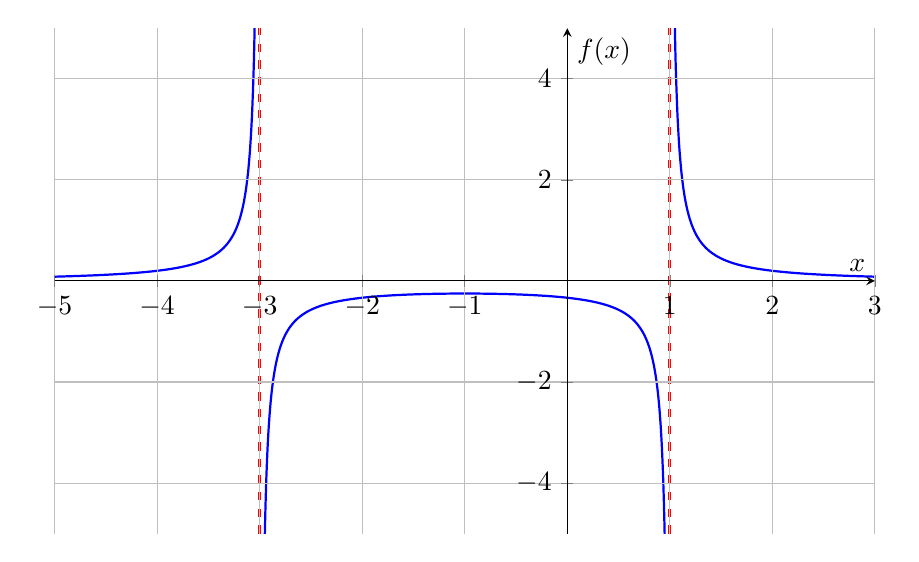
\begin{tikzpicture}
            \begin{axis}[
                axis lines = middle,
                xlabel = $x$, ylabel = {$f(x)$},
                xmin = -5, xmax = 3,
                ymin = -5, ymax = 5,
                grid = both,
                width = 12cm,
                height = 8cm,
                samples = 10,
                smooth,
                axis on top,
            ]
            \addplot[blue, thick, domain=-5:-3.01, samples=100] {1/((x-1)*(x+3))};
            \addplot[blue, thick, domain=-2.99:0.99, samples=300] {1/((x-1)*(x+3))};
            \addplot[blue, thick, domain=1.01:3, samples=100] {1/((x-1)*(x+3))};
            
            \draw[dashed, red, very thick] (axis cs:-3,\pgfkeysvalueof{/pgfplots/ymin}) -- (axis cs:-3,\pgfkeysvalueof{/pgfplots/ymax});
            \draw[dashed, red, very thick] (axis cs:1,\pgfkeysvalueof{/pgfplots/ymin}) -- (axis cs:1,\pgfkeysvalueof{/pgfplots/ymax});
            \end{axis}
        \end{tikzpicture}
    \end{center}
    
\end{solution}

\begin{problem}
    For the function, $g$, define below, find it's vertical asymptotes.
    \[
        g(x) = \frac{3}{x^2 + 1}
    \]
\end{problem}
Give it a shot. When you're done or get stuck, read ahead to the solution.
\begin{solution}
    Just like before, we can see that the denominator cannot equal $0$. So we can set it to $0$ and solve.
    \[
    x^2 + 1 = 0
    \]
    However, there's something different about this solution. If we let $a = 1$, $b = 0$, and $c = 1$, we can see that the discriminant ($b^2 - 4ac$) is less than $0$.
    \[
        0 - 4(1)(1) = -4
    \]
    This means that there are no real solutions to this quadratic. When the denominator set equal to $0$ has no real solutions, it means the function has no vertical asymptotes.

    \begin{center}
        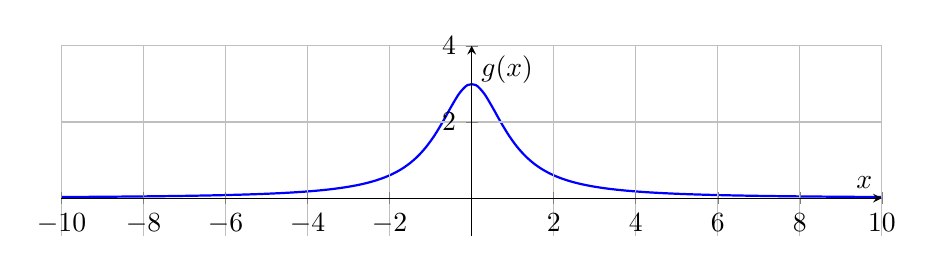
\begin{tikzpicture}
            \begin{axis}[
                axis lines = middle,
                xlabel = $x$, ylabel = {$g(x)$},
                xmin = -10, xmax = 10,
                ymin = -1, ymax = 4,
                grid = both,
                width = 12cm,
                height = 4cm,
                samples = 10,
                smooth,
                axis on top,
            ]
            \addplot[blue, thick, domain=-10:10, samples=100] {3/(x^2 + 1)};
            \end{axis}
        \end{tikzpicture}
    \end{center}
\end{solution} % Subsection 1.1.1 - Vertical Asymptotes
\clearpage\subsection{Horizontal Asymptotes}
Horizontal asymptotes come about because of a range restriction. To be more accurate, horizontal asymptotes are a result of the end behavior of a function as $x$ approaches $\pm \infty$. Just like with vertical asymptotes, we can solve for the range of a function and observe its behavior as it aproaches the range restrictions. Conversely, we can use values from the domain that, when plugged into the function, gradually bring the function closer and closer to its range restriction.

What does this mean? Take the example $g(x) = \dfrac{1}{x}$. Earlier in the section on asymptotes ("1.1 Asymptotes"), we calculated $g(x)$ for extremely large values of $x$. As the value of $x$ increased, the output $g(x)$ decrased. In fact, it slowly got closer and closer to its domain restriction: $y \ne 0$. Let's look at some example problems.

\begin{problem}
    For the function, $f$, defined below, find it's horizontal asymptotes.
    \[
        f(x) = \frac{1}{(x - 1)(x + 3)}
    \]
\end{problem}

\begin{solution}
    The function $f(x)$ cannot equal $0$, regardless of what the denominator is, because the numerator will \textbf{always} be $1$. Therefore, we can say that this method has a range of $y \neq 0$. To see if this is indeed a horizontal asymptote, let's plug some large values and see what happens.
    \[
    \begin{aligned}
        f(100) &\approx 0.0000981
        f(10000) &&\approx 0.000000009998 \\
        f(-100) &\approx 0.000102
        f(-10000) &&\approx 0.00000001
    \end{aligned}
    \]
    We can see that plugging large values of $x$ gets us closer and closer to our range restriction $y \neq 0$. Since that is our only range restriction, we can say that the function $f(x)$ has a horizontal asymptote of $y = 0$.

    \begin{center}
        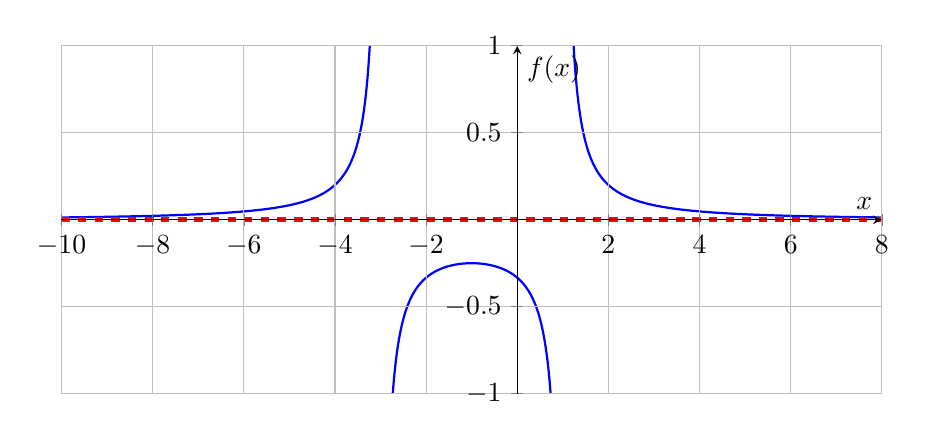
\begin{tikzpicture}
            \begin{axis}[
                axis lines = middle,
                xlabel = $x$, ylabel = {$f(x)$},
                xmin = -10, xmax = 8,
                ymin = -1, ymax = 1,
                grid = both,
                width = 12cm,
                height = 6cm,
                samples = 10,
                smooth,
                axis on top,
            ]
            \addplot[blue, thick, domain=-10:-3.01, samples=300] {1/((x-1)*(x+3))};
            \addplot[blue, thick, domain=-2.99:0.99, samples=300] {1/((x-1)*(x+3))};
            \addplot[blue, thick, domain=1.01:8, samples=300] {1/((x-1)*(x+3))};
            \addplot[red, dashed, ultra thick, domain=-10:8, samples=10] {0};
            \end{axis}
        \end{tikzpicture}
    \end{center}
\end{solution}

\begin{problem}
    For the function, $g$, define below, find it's horizontal asymptotes.
    \[
        g(x) = \frac{3x^2 + 5}{x^2 + 1}
    \]
\end{problem}

Your first instinct would be to look for the range. While that \textit{is} a valid strategy, you'll notice that it's quite cumbersome. I mean... Where do you even start? Throwing a bunch of large values of $x$ \textit{would} give the answer, but let's think of a better way to explain this. It's crucial that we explore this further because it reveals a trick we can use to solve any problem like this in an instant.

\begin{solution}
    First, let's plug the number $1$ into this function.
    \[
        g(1) = \frac{3(1)^2 + 5}{(1)^2 + 1} = \frac{3 + 5}{1 + 1}
    \]
    When we plug $x = 1$ into this function, that $+5$ and $+1$ in the numerator and denominator \textit{really} change the answer. We're jumping from $5$ to $8$ in the numerator and from $1$ to $2$ in the denominator. Now, let's try plugging a larger number, like $100$.
    \[
        g(100) = \frac{3(100)^2 + 5}{(100)^2 + 1} = 
        \frac{3(10000) + 5}{10000 + 1} = \frac{30000 + 5}{10000 + 1}
    \]\clearpage
    Take a look at this. The $+5$ and $+1$ in the numerator and denominator don't really do anything anymore. Yeah, they increase the number, but compared to how large $30000$ and $10000$ are, they're basically nothing. It should be clear, now, that plugging larger and larger numbers into $x$ makes the $+5$ and $+1$ more and more insignificant. As $x$ increases, we're basically looking at
    \[
        g(x) = \frac{3x^2}{x^2} = \boxed{3}
    \]
    Sure enough, that is our asymptote. The horizontal asymptote of $g(x)$ is $y = 3$.

    \begin{center} {\vspace{-0.75cm}}
        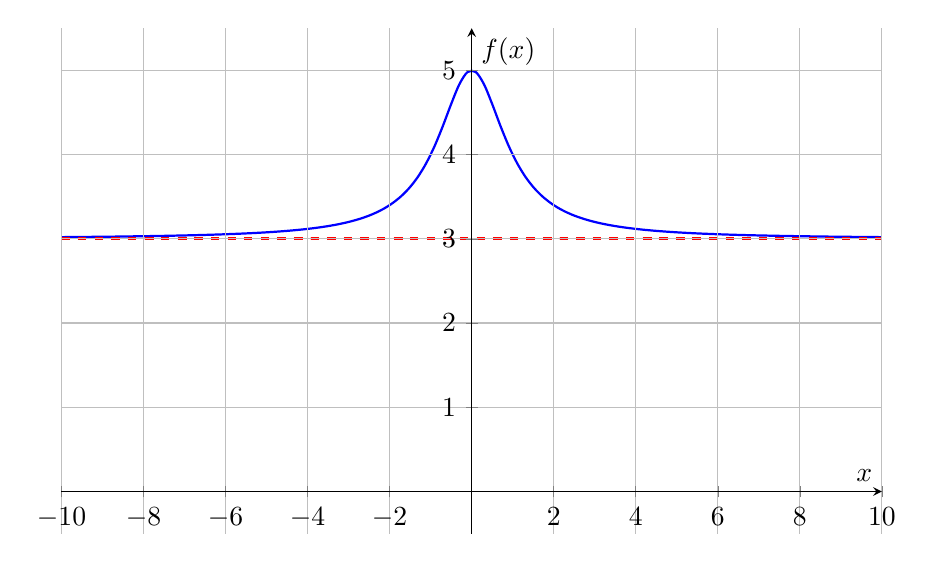
\begin{tikzpicture}
            \begin{axis}[
                axis lines = middle,
                xlabel = $x$, ylabel = {$f(x)$},
                xmin = -10, xmax = 10,
                ymin = -0.5, ymax = 5.5,
                grid = both,
                width = 12cm,
                height = 8cm,
                samples = 50,
                smooth,
                axis on top,
            ]
            \addplot[blue, thick, domain=-10:10, samples=100] {(3 * x^2 + 5) / (x^2 + 1)};
            \addplot[red, dashed, very thick, domain=-10:10, samples=10] {3};
            \end{axis}
        \end{tikzpicture}
    \end{center}
\end{solution}

If the degree of the numerator and denominator are the same, the horizontal asymptote is determined by dividing the coefficient of the highest degree in the numerator by that of the denomianator. % Subsection 1.1.2 - Horizontal Asymptotes
\clearpage\subsection{Polynomial Asymptotes}
Polynomial asymptotes, unlike vertical and horizontal, are quite tricky. They only occur when the degree of the polynomial in the numerator is greater than that in the denominator. It's not easy to define them using a domain and range because they don't conform strictly to the domain (vertical asymptote) or range (horizontal asymptote). We must, instead, be a little more creative.

Let's remember what division does to a number. Take something like this, for example: $10 \div 3$. In many cases, the number you're dividing by, the divisor, doesn't fit evenly into the number you're dividing, the dividend. In such cases, you are left with a remainder that can be written as a fraction, like so:
\[
3 + \frac{1}{3} \text{.}
\]
The answer we get is such that multiplying it by $3$ gets us back to the original number, $10$. This is true with polynomials, too.

If we allow the following to be true: \\
$f(x)$ - Dividend\\
$g(x)$ - Divisor\\
$q(x)$ - Quotient\\
$r(x)$ - Remainder

Then we can say that the solution to polynomial long division can be expressed like so:
\[
\frac{f(x)}{g(x)} = q(x) + \frac{r(x)}{g(x)}
\]
\clearpage
If we let:\\
$f(x) = x^2$ \\
$g(x) = x + 1$

We get the following solution:
\[
\begin{array}{r|rrrrr}
& x & -1 & &\\ \cline{2-4}
x + 1 & x^2 & 0\\
& -(x^2 & x) & & \\ \cline{2-3}
& & -x & 0\\ 
& & -(-x & -1) \\ \cline{3-5}
& & & 1
\end{array}
\]
In this case, $q(x) = x - 1$ and $r(x) = 1$. Thus, we can write the solution
\[
\frac{x^2}{x + 1} = x - 1 + \frac{1}{x + 1} \text{.}
\]
Notice how, in the $\dfrac{r(x)}{g(x)}$ term, the $x$ is in the denominator. As $x$ grows larger and larger, like to $10000$ or $\infty$, that term becomes smaller and smaller.
\[
    \frac{\text{small number}}{\text{big number}} = \text{small number}
\]
As that term reaches $0$, we are left with $q(x)$, which we established will never actually reach the rational function defined as $\dfrac{f(x)}{g(x)}$. So, no matter what values of $x$ we put in there, and no matter how close $q(x)$ might get to $\dfrac{f(x)}{g(x)}$, it will never touch it. \textbf{That is the definition of an asymptote.}

\begin{definition} % Customized Theorem Envirnment
    Given a dividend, $f(x)$, and a divisor of a lower degree, $g(x)$, written as a rational function, $y = \dfrac{f(x)}{g(x)}$, the polynomial asymptote is defined as 
    \[
        y = q(x) \text{,}
    \]
     where $q(x)$ is the quotient obtained from dividing $\dfrac{f(x)}{g(x)}$.
\end{definition}
\clearpage
While this is true for all rational functions with polynomials in the numerator and denominator, the one you'll most commonly see is a rational function where the degree of the numerator is $1$ greater than the denominator. This is also called a \textbf{slant} or \textbf{oblique} asymptote.

Let's look at a practice problem together.
\begin{problem}
    Find all the asymptotes for the rational function
    \[
        f(x) = \frac{3x^2 + x - 10}{x - 5} \text{.}
    \]
    \textit{Note that $f(x)$, in this case, is the entire rational function and \textbf{not} the dividend.}
\end{problem}

\begin{solution}
    We need to find the quotient of this rational function. Beacuse the denominator has a degree of $1$, we can use synthetic division.
    \[
    \begin{aligned}
        \begin{array}{r|rrr}
            5 & 3 & 1  & -10 \\
            &   & 15 & 90  \\ \cline{2-4}
            & 3 & 16 & 80
        \end{array} \\
        q(x) = 3x + 16
    \end{aligned}
    \]
    That's the first asymptote. There is a second hiding in the denominator. If we set that equal to $0$, we can solve for a vertical asymptote as well.
    \[
        x - 5 = 0 \Longrightarrow x = 5
    \]
    \begin{center}
        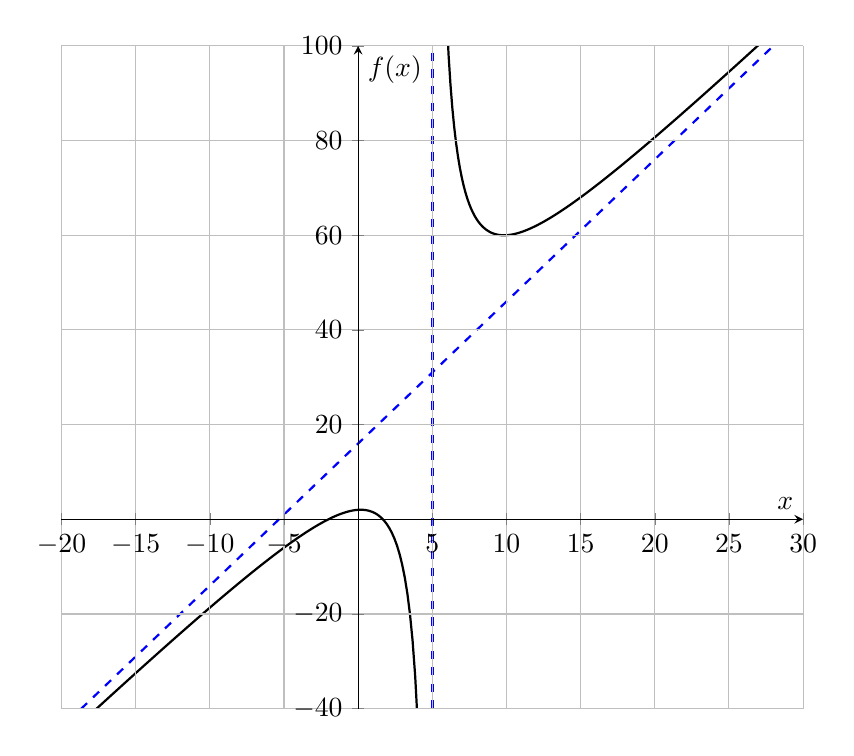
\begin{tikzpicture}
            \begin{axis}[
                axis lines = middle,
                xlabel = $x$, ylabel = {$f(x)$},
                xmin = -20, xmax = 30,
                ymin = -40, ymax = 100,
                grid = both,
                width = 11cm,
                height = 10cm,
                axis on top,
            ]
            % Left branch (x < 5)
            \addplot[black, thick, domain=-30:4.9, samples=200, restrict y to domain=-44:5] 
                {(3*x^2 + x - 10)/(x-5)};
            % Right branch (x > 5)
            \addplot[black, thick, domain=5.1:30, samples=200, restrict y to domain=55:106] 
                {(3*x^2 + x - 10)/(x-5)};
            % Slant asymptote y = 3x + 16
            \addplot[blue, dashed, thick, domain=-30:30, samples=10] {3*x + 16};
            \draw[dashed, blue, very thick] (axis cs:5,\pgfkeysvalueof{/pgfplots/ymin}) -- (axis cs:5,\pgfkeysvalueof{/pgfplots/ymax});
            \end{axis}
        \end{tikzpicture}
    \end{center}
\end{solution}
 % Subsection 1.1.3 - Polynomial Asymptotes

\chapter{Transformations}
\vspace{-1cm}
Up to this point, we've just been drawing functions and finding key details about them (asymptotes, domain, range). Now it's time to move functions around and warp them in all kinds of ways. You probably learned how to do this back in Algebra II (or Integrated III). The goal here is to really cement that understand.

\noindent If $f(x)$ is the parent function, these are what the transformations look like:
\[
    af\left(\frac{1}{b}(x - h)\right) + k
\]
\begin{itemize}
    \item $h$ - Horizontal shift (positive = right)
    \item $k$ - Vertical Shift (positive = up)
    \item $a$ - Stretching and Shrinking along the vertical axis
    \begin{itemize}
        \item Larger Values = More Vertical Stretching
    \end{itemize}  
    \item $b$ - Stretching and Shrinking along the horizontal axis
    \begin{itemize}
        \item Larger Values = More Horizontal Stretching
    \end{itemize}
\end{itemize}
\textit{Note: Some texts use $b$ instead of $\dfrac{1}{b}$. When using $b$, larger values of $b$ horizontally \textbf{compress} instead of stretch.}

Let's try to understand why each of these variables transform the function the way they do. % Chapter 2 - Transformations
\section{Vertical Shifts}
The easiest of the transformations to consider is $k$. This variable vertically shifts the function by its value. For example, if $f(x) = x$, then $g(x) = x + 1$, where $k = 1$, is simply the function $f(x)$ but moved up a unit. In the same manner, a function $h(x) = x - 1$, where $k = -1$, is the function $f(x)$ moved down a unit.

\begin{center}
    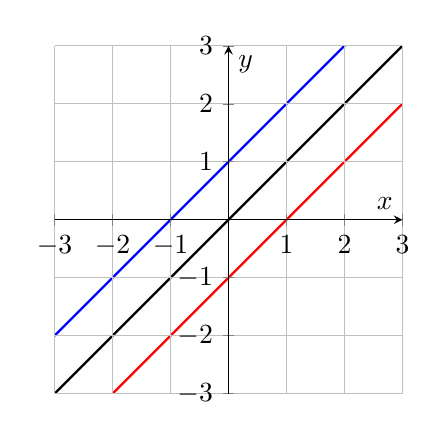
\begin{tikzpicture}
        \begin{axis} [
            axis lines=middle,
            xlabel = $x$, ylabel = {$y$},
            xmin = -3, xmax = 3,
            ymin = -3, ymax = 3,
            xtick distance={1}, ytick distance={1},
            grid = both,
            width = 6cm,
            height = 6cm,
            smooth,
            axis on top
        ]

            \addplot[black, thick, smooth, domain = -3:3, samples = 100]{x};
            \addplot[blue, thick, smooth, domain = -3:3, samples = 100]{x + 1};
            \addplot[red, thick, smooth, domain = -3:3, samples = 100]{x - 1};
        \end{axis}
    \end{tikzpicture}\\
    $f(x) = x$ (Black), 
    $g(x) = x + 1$ (Blue), 
    $h(x) = x - 1$ (Red)
\end{center}
A vertical shift moves all parts of a funtion the specified number of units up or down. That includes asymptotes. For example, if the function I'll redefine as $f(x) = \dfrac{1}{x}$ has a horizontal asymptote of $y = 0$, the new redefined function $g(x) = \dfrac{1}{x} + 1$ wil have a horizontal asymptote of $y = 1$.
\begin{definition}
Given a function $f(x)$ and a vertical shift $k$, the new function $g(x) = f(x) + k$ is the function $f(x)$ vertically translated $k$ units.
\begin{itemize}
    \item When $k < 0$, $f(x)$ moves in the negative $y$ direction (down).
    \item When $k > 0$, $f(x)$ moves in the positive $y$ direction (up).
    \item When $k = 0$, $f(x) = g(x)$. The function does not move.
\end{itemize} 
\end{definition}  % Section 2.1 - Vertical Shift
\clearpage\section{Vertical Stretches}
A close second in terms of simplicity is the vertical stretch, represented by the letter $a$. This function multiplies every output of a function by its value. For example, if $f(x) = x$, the function $g(x) = 2x$, where $a = 2$, means that every value plugged into $g(x)$ is doubled. Likewise, if we set $a = \dfrac{1}{2}$, every value plugged into a new function $h(x) = \dfrac{1}{2}x$ is halved.
\begin{center}
    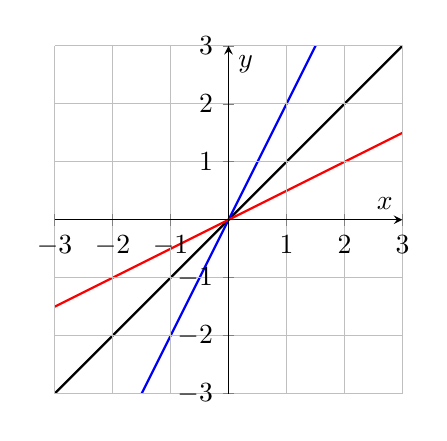
\begin{tikzpicture}
        \begin{axis} [
            axis lines=middle,
            xlabel = $x$, ylabel = {$y$},
            xmin = -3, xmax = 3,
            ymin = -3, ymax = 3,
            xtick distance={1}, ytick distance={1},
            grid = both,
            width = 6cm,
            height = 6cm,
            smooth,
            axis on top
        ]

            \addplot[black, thick, smooth, domain = -3:3, samples = 100]{x};
            \addplot[blue, thick, smooth, domain = -3:3, samples = 100]{2 * x};
            \addplot[red, thick, smooth, domain = -3:3, samples = 100]{(1 / 2) * x};
        \end{axis}
    \end{tikzpicture}\\
    $f(x) = x$ (Black), 
    $g(x) = 2x$ (Blue),
    $h(x) = \dfrac{1}{2}x$ (Red) \\
    \textit{Note that $a$ for a linear function is its slope.}
\end{center}

\begin{definition}
    Given a function $f(x)$ and a vertical stretch $a$, the new function $g(x) = af(x)$ is the function where every value in the range of $f$ is multiplied by $a$.
    \begin{itemize}
        \item When $a > 1$, stretching occurs.
        \item When $0 < a < 1$, compression occurs.
        \item When $a = 1$, the function is unaffected. 
        \item When $a = 0$, the function is a horizontal line.
    \end{itemize}
\end{definition}
 % Section 2.1 - Vertical Stretch
\clearpage\subsection{Vertical Reflection}
A vertical reflection is achieved when $a$ is negative. A negative value for $a$ means every value for a function $f(x)$ that used to be positive becomes negative. For example, when $a = 1$ for the function $f(x) = x$, inputting $x = 1$ produces $y = 1$. However, for a function $g(x) = -x$, where $a = -1$, plugging $x = 1$ produces $y = -1$.
\begin{center}\vspace{-0.25cm}
    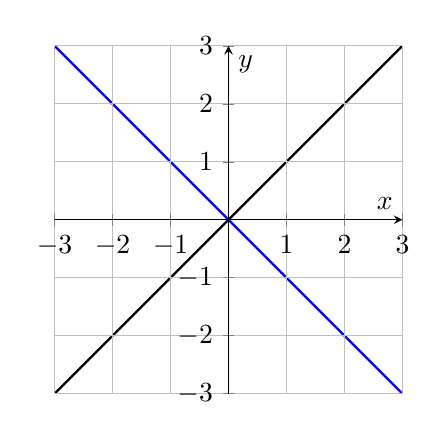
\begin{tikzpicture}
        \begin{axis} [
            axis lines=middle,
            xlabel = $x$, ylabel = {$y$},
            xmin = -3, xmax = 3,
            ymin = -3, ymax = 3,
            xtick distance={1}, ytick distance={1},
            grid = both,
            width = 6cm,
            height = 6cm,
            smooth,
            axis on top
        ]

            \addplot[black, thick, smooth, domain = -3:3, samples = 100]{x};
            \addplot[blue, thick, smooth, domain = -3:3, samples = 100]{-1 * x};
        \end{axis}
    \end{tikzpicture}\\
    $f(x) = x$ (Black), 
    $g(x) = -x$ (Blue),
\end{center}
\begin{definition}
    Given a function $f(x)$, a vertical reflection, also called a reflection along the $x-axis$ or $y = 0$, occurs when $a < 0$. For the function $g(x) = af(x)$, all values in the range are switched from positive to negative (and vice versa), and then stretched by $|a|$.
    \begin{itemize}
        \item When $a < -1$, vertical stretching in the negative direction occurs.
        \item When $-1 < a < 0$, vertical compressing in the negative direciton occurs.
        \item When $a = -1$, the function is reflected without stretching or compressing.
    \end{itemize}
\end{definition} % Subsection 2.1.1 - Vertical Reflection
\clearpage\section{Horizontal Shifts}
Now for the slightly trickier transformations. This first one is the horizontal shift, represented by the letter $h$. A horizontal shift, like a vertical one, moves the function left or right. For example, if $f(x) = x^2$, a horizontal shift one unit to the right would result in a new function $g(x) = (x - 1)^2$, where $h = 1$. 

Herein lies the confusion: If we're subtracting $x$ by $1$, why does the function move in the positive $x$ direction? Aren't negative values of $x$ on the left?

Negative values \textit{are} on the left, but it shifts to the right because the result that would've normally been produced by $f(x)$ is now produced by some larger input of $x$. 

$f(2) = 4$ because when you square $2$ you get $4$. But if you want $g(x)$ to also produce $4$, you have to use $g(3)$.
\[
    g(3) = (3 - 1)^2 = (2)^2 = 4
\]
To produce the same result, you had to input a larger value of $x$. The best example of this is getting the functions to result in $0$.
\begin{align*}
    f(0) &= (0)^2 = 0 && \text{Point at }(0, 0)\\
    g(1) &= (1 - 1)^2 = (0)^2 = 0 && \text{Point at }(1, 0)
\end{align*}
Notice that the difference for when $f(x) = g(x) = 4$ and $f(x) = g(x) = 0$, the difference in input for $f(x)$ and $g(x)$ is the value of $h$. It can then be proposed that increasing the value of $h$ to, say, $h = 3$, plugging $3$ into $h(x) = (x - 3)^2$ will produce $0$.
\[
    h(3) = (3 - 3)^2 = (0)^2 = 0 \qquad \text{Point at }(3, 0)
\]
\begin{center}
    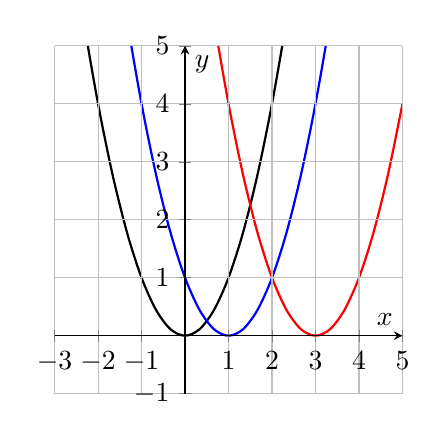
\begin{tikzpicture}
        \begin{axis} [
            axis lines=middle,
            xlabel = $x$, ylabel = {$y$},
            xmin = -3, xmax = 5,
            ymin = -1, ymax = 5,
            xtick distance={1}, ytick distance={1},
            grid = both,
            width = 6cm,
            height = 6cm,
            smooth,
            axis on top
        ]
        \addplot[black, thick, domain=-3:5] {x^2};
        \addplot[blue, thick, domain=-3:5] {(x - 1)^2};
        \addplot[red, thick, domain=-3:5] {(x - 3)^2};
        \end{axis}
    \end{tikzpicture}\\
    $f(x) = x^2$ (Black), $g(x) = (x - 1)^2$ (Blue), $h(x) = (x - 3)^2$ (Red)
\end{center}
\begin{definition}
    Given a function $f(x)$ and a horizontal shift $k$, the new function $g(x) = f(x - 1)$ is the function of $f(x)$ horizontally translated $h$ units.
    \begin{itemize}
        \item When $h < 0$, $f(x)$ moves in the negative $x$ direction (left).
        \item When $h > 0$, $f(x)$ moves in the positive $x$ direction (right).
        \item When $h = 0$, $f(x) = g(x)$. The function does not move.
    \end{itemize}
\end{definition} % Section 2.1 - Horizontal Shift
\clearpage \section{Horizontal Stretching}
Horizontal stretching is by far the most confusing. At the beginning of this chapter, I wrote $\dfrac{1}{b}(x - h)$ and noted that some texts use $b$ instead of $\dfrac{1}{b}$. In this section, I'll be sure to clarify exactly what adding a value in front of those parentheses does to the function and explain the differences between $b$ and $\dfrac{1}{b}$. 

Let's define a function $f(x) = x^2$. I'll now create a table with three columns: one for the $x$ value plugged into the function, one for the value of $x$ after $b$ is applied, and one for the output of the function. In this case, $b = 1$, so the table of $f(x)$ looks something like this:
\begin{center}
    \begin{tabular}{ c | c | c }
        $x$ & $1x$ & $f(x)$ \\
        \hline
        $-2$ & $-2$ & $4$ \\
        \hline
        $-1$ & $-1$ & $1$ \\
        \hline
        $0$ & $0$ & $0$ \\
        \hline
        $1$ & $1$ & $1$ \\
        \hline
        $2$ & $2$ & $4$
    \end{tabular}\\
\end{center}
Now let's look at another function $g(x) = (2x)^2$.
\begin{center}
    \begin{tabular}{ c | c | c }
        $x$ & $2x$ & $g(x)$ \\
        \hline
        $-2$ & $-4$ & $16$ \\
        \hline
        $-1$ & $-2$ & $4$ \\
        \hline
        $0$ & $0$ & $0$ \\
        \hline
        $1$ & $2$ & $4$ \\
        \hline
        $2$ & $4$ & $16$
    \end{tabular}\\
\end{center}
Notice how an input of $2$ all of a sudden becomes $4$. This is \textit{almost} like a vertical stretch. If this \textit{had} been a vertical stretch (i.e. $y = 2x^2$), an input of $2$ would produce $y = 8$. But we got $16$ this time with $g(x)$. Instead of imagining it as a stretch upward, imagine the graph being smushed together so that the points are more tightly packed near the $y$-axis line ($x = 0$).

Btw, you could totally see it as something similar to a vertical stretch. Your teacher might not like it (and neither do I) because doing so would make it easy to confuse the vertical stretch $2x^2$ with the "vertical stretch" $(2x)^2$. So, just for teacher's and your own sanity, just think of $(2x)^2$ as a horizontal compression.

Let's look at these functions on a graph!
\begin{center}
    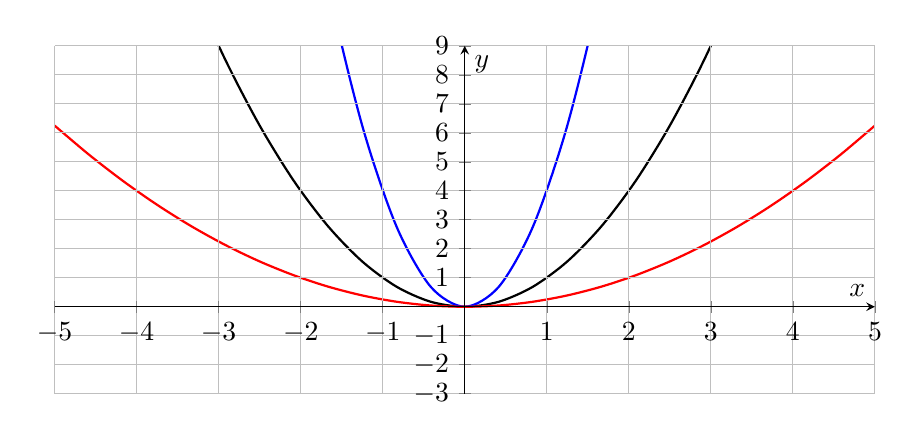
\begin{tikzpicture}
        \begin{axis} [
            axis lines=middle,
            xlabel = $x$, ylabel = {$y$},
            xmin = -5, xmax = 5,
            ymin = -3, ymax = 9,
            xtick distance={1}, ytick distance={1},
            grid = both,
            width = 12cm,
            height = 6cm,
            smooth,
            axis on top
        ]
        \addplot[black, thick, domain=-5:5] {x^2};
        \addplot[blue, thick, domain=-5:5] {(2 * x)^2};
        \addplot[red, thick, domain=-5:5] {((1/2) * x)^2};
        \end{axis}
    \end{tikzpicture}\\
    $f(x) = x^2$ (Black), $g(x) = (2x)^2$ (Blue), $\displaystyle h(x) = \left(\dfrac{1}{2}x\right)^2$ (Red)
\end{center}

\begin{definition}
    Given a function $f(x)$ and a horizontal stretch $b$, the new function $\displaystyle g(x) = f\left(\dfrac{1}{b}x\right)$ is the function of $f$ horizontally stretched by a factor of $b$.
    \begin{itemize}
        \item When $b > 1$, horizontal stretching occurs.
        \item When $0 < b < 1$, horizontal compression occurs.
        \item When $b = 1$, the function is unaffected.
        \item When $b = 0$, the function is undefined.
    \end{itemize}
\end{definition} % Section 2.1 - Horizontal Stretch
\clearpage\subsection{Horizontal Reflections}
A horizontal reflection is achieved when $b$ is negative. A negative value for $b$ means every input for a function $f(x)$ that used to be positive becomes negative. For example, when $b = 1$ for the function $f(x) = \dfrac{1}{x}$, inputting $x = 1$ produces $y = 1$. However, for a function $g(x) = \dfrac{1}{-x}$, where $b = -1$, plugging $x = 1$ produces $y = -1$.
\begin{center}\vspace{-0.25cm}
    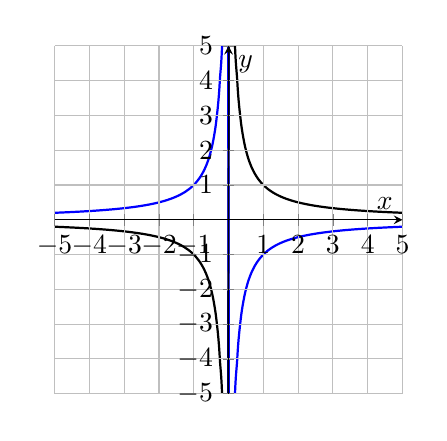
\begin{tikzpicture}
        \begin{axis} [
            axis lines=middle,
            xlabel = $x$, ylabel = {$y$},
            xmin = -5, xmax = 5,
            ymin = -5, ymax = 5,
            xtick distance={1}, ytick distance={1},
            grid = both,
            width = 6cm,
            height = 6cm,
            smooth,
            axis on top
        ]

            \addplot[black, thick, smooth, domain = -5:5, samples = 100]{1 / x};
            \addplot[blue, thick, smooth, domain = -5:5, samples = 100]{1 / (-1 * x)};
        \end{axis}
    \end{tikzpicture}\\
    $f(x) = \dfrac{1}{x}$ (Black), 
    $f(x) = \dfrac{1}{-x}$ (Blue),
\end{center}

\begin{definition}
    Given a function $f(x)$, a vertical reflection, also called a reflection along the $y$-axis or $x = 0$, occurs when $b < 0$. For the function $\displaystyle g(x) = f\left(\frac{1}{b}x \right)$, all values in the domain are switched from positive to negative (and vice versa), and stretched by a factor of $\left|b\right|$.
    \begin{itemize}
        \item When $b < -1$, horizontal stretching in the negative direction occurs.
        \item When $-1 < a < 0$, horizontal compressing in the negative direction occurs.
        \item When $a = -1$, the function is reflected without stretching or compressing.
    \end{itemize}
\end{definition} % Subsection 2.1.1 - Horizontal Reflection
\clearpage
\section{Practice Problems}
Let's do some practice problems, shall we? I'll only give a couple, each increasing in difficulty.

\begin{problem}
    Let the function $f$ be $f(x) = x^2$. Translate (move) this function $2$ units to the right and $1$ unit down. Write your answer as a new function $g$.
\end{problem}
\begin{solution}
    We're given two translations: A horizontal translation $h$ and a vertical translation $k$. We're asked to move this function two units to the right, meaning $h = 2$. We're then asked to move this function $1$ unit down, meaning $k = -1$. Apply these to the template $g(x) = f(x - h) + k$.
    Plugging these into the function yields the answer $\boxed{g(x) = (x - 2)^2 - 1}$.
\begin{center}
    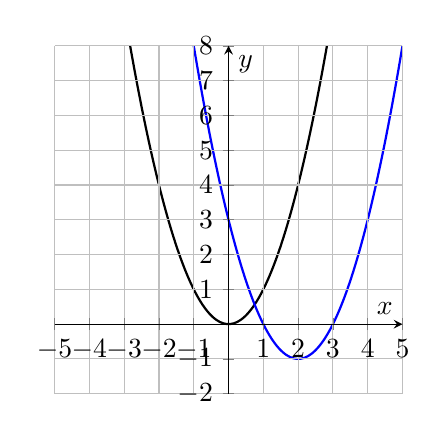
\begin{tikzpicture}
        \begin{axis} [
            axis lines=middle,
            xlabel = $x$, ylabel = {$y$},
            xmin = -5, xmax = 5,
            ymin = -2, ymax = 8,
            xtick distance={1}, ytick distance={1},
            grid = both,
            width = 6cm,
            height = 6cm,
            smooth,
            axis on top
        ]

            \addplot[black, thick, smooth, domain = -5:5, samples = 100]{x^2};
            \addplot[blue, thick, smooth, domain = -5:5, samples = 100]{(x - 2)^2 - 1};
        \end{axis}
    \end{tikzpicture}\\
    $f(x) = x^2$ (Black), 
    $g(x) = (x - 2)^2 - 1$ (Blue),
\end{center}
\end{solution}\clearpage
\begin{problem}
    Let the function $f$ be $f(x) = \sqrt{x}$. Apply a vertial stretch with a factor of $3$ and horizontal stretch with a factor of $\frac{1}{2}$. Write your answer as a new function $g$.
\end{problem}
\begin{solution}
We're given two transformations: A vertial stretch $a$ and a horizontal stretch $b$. We're asked to vertically stretch this function by a factor of $3$, meaning $a = 3$, and horizontally stretch this function by a factor of $\frac{1}{2}$, meaning $b = \frac{1}{2}$. Apply these to the template $g(x) = af\left(\dfrac{1}{b}x \right)$. 

The vertical stretch is easy, just slap the $3$ in for $a$. The horizontal stretch, on the other hand, is more tricky. We know that $b = \dfrac{1}{2}$, but plugging that in gives $\dfrac{1}{1/2}$. This is a complex fraction and serves only to complicate things. To get rid of this, we multiply the numerator and denominator by the reciporical of the denominator.
\[
    \frac{1}{\frac{1}{2}}\cdot \frac{\frac{2}{1}}{\frac{2}{1}} =
    1 \cdot \frac{2}{1} = 1 \cdot 2 = 2
\]
Thus, our final answer is $\boxed{g(x) = 3\sqrt{2x}}$.
\begin{center}
    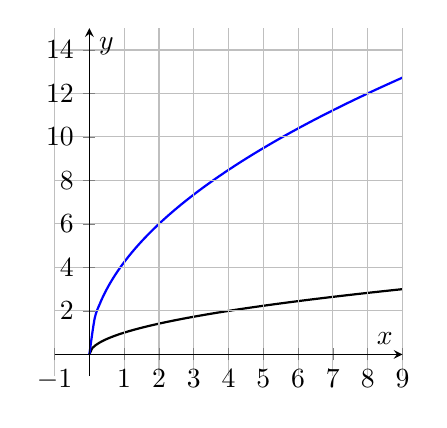
\begin{tikzpicture}
        \begin{axis} [
            axis lines=middle,
            xlabel = $x$, ylabel = {$y$},
            xmin = -1, xmax = 9,
            ymin = -1, ymax = 15,
            xtick distance={1}, ytick distance={2},
            grid = both,
            width = 6cm,
            height = 6cm,
            smooth,
            axis on top
        ]

            \addplot[black, thick, smooth, domain = 0:9, samples = 100]{sqrt(x)};
            \addplot[blue, thick, smooth, domain = 0:15, samples = 100]{3 * sqrt(2 *x)};
        \end{axis}
    \end{tikzpicture}\\
    $f(x) = x^2$ (Black), 
    $g(x) = (x - 2)^2 - 1$ (Blue),
\end{center}
\end{solution} \clearpage
\begin{problem}
    Let the function $f$ be $f(x) = \dfrac{1}{x}$. Translate the function $3$ units to the left and $5$ units up. Transform the function with a vectical stretch factor of $2$ and horizontal stretch factor of $3$. Reflect the function over the $y$-axis. Write your answer as a new function $g$.
\end{problem}
\begin{solution}
    There are a lot of things we need to do to this function, so let's list them one at a time.
    \begin{itemize}
        \item Move $3$ units left ($h = 3$).
        \item Move $5$ units up ($k = 5$).
        \item Vertically stretch by a factor of $2$ ($a = 2$).
        \item Horizontally stretch by a factor of $3$ ($b = 3$).
        \item Reflect over the $y$-axis (We'll worry about this later).
    \end{itemize}
    With what we've gathered so far, we can create a template:
    \begin{align*}
        g(x) &= 2f\left(\frac{1}{3}(x - 3) \right) + 5 \\
        \intertext{From here, we can plug everything in}
        g(x) &= 2\left(\frac{1}{\frac{1}{3}(x - 3)} \right) + 5
    \end{align*}
    Now we can reflect over the $y$-axis. Remember that the $y$-axis is the line $x = 0$. It's the vertical line that goes straight through the $xy$-plane. Since we're reflecting from left to right, we must multiply $b$ by $-1$. This gives
    \[
        g(x) = 2\left(\frac{1}{-\frac{1}{3}(x - 3)} \right) + 5 \text{.}
    \]
    Now, we begin solving:
    \begin{align*}
    g(x) &= \frac{2}{-\frac{1}{3}(x - 3)}\left(\frac{\frac{3}{1}}{\frac{3}{1}} \right) + 5 \\
    &= \frac{6}{-(x - 3)} + 5 \\
    &= 5 - \frac{6}{x - 3}
    \end{align*}
\begin{center}
    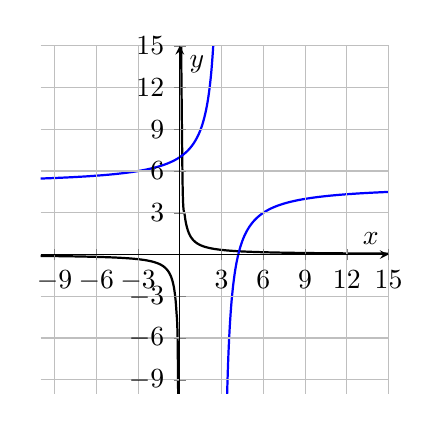
\begin{tikzpicture}
        \begin{axis} [
            axis lines=middle,
            xlabel = $x$, ylabel = {$y$},
            xmin = -10, xmax = 15,
            ymin = -10, ymax = 15,
            xtick distance={3}, ytick distance={3},
            grid = both,
            width = 6cm,
            height = 6cm,
            smooth,
            axis on top
        ]

            \addplot[black, thick, smooth, domain = -10:-0.05, samples = 100]{1 / x};
            \addplot[black, thick, smooth, domain = 0.05:15, samples = 100]{1 / x};
            \addplot[blue, thick, smooth, domain = -10:2.8, samples = 100]{5 - (6 / (x - 3))};
            \addplot[blue, thick, smooth, domain = 3.1:15, samples = 100]{5 - (6 / (x - 3))};
        \end{axis}
    \end{tikzpicture}\\
    $f(x) = \frac{1}{x}$ (Black), 
    $g(x) = 5 - \frac{6}{x - 3}$ (Blue),
\end{center}
Note that you could also write this function as
\[
    g(x) = \frac{6}{3 - x} + 5 \text{.}
\]
and get the same result. That's how I'd write it. You could also just leave it as
\[
    g(x) = \frac{6}{-(x - 3)} + 5 \Longrightarrow \boxed{g(x) = -\frac{6}{x - 3} + 5} \text{.}
\]
It's all stylistic/presentation preferences.
\end{solution}
\chapter{Function Composition}
Function composition is esentially the operations (i.e. addition, subtraction, multiplication, division) with functions instead of numbers and variable. It may \textit{seem} intimidating, but it's really super easy. I'll be sure to take it one step at a time. But you'll realize that it's really just the basic operations written differently. In this section, I'll be covering:
\begin{itemize}
    \item Function addition $(f + g)(x)$
    \item Function subtraction $(f - g)(x)$
    \item Function multiplication $(f \cdot g)(x)$
    \item Function division $\displaystyle \left(\frac{f}{g} \right)(x)$
\end{itemize}
Let's begin with addition, since it's the simplest one.
\clearpage\section{Function Addition}
Function addition is exactly what it sounds like. Given a function $f(x)$ and $g(x)$, you just add them together. So, if $f(x) = 3x$ and $g(x) = 2x^2$, $(f + g)(x) = 2x^2 + 3x$. That's it. The only tricky part is managing the domain of both functions. 

In the example from just now, the domain of $f(x)$ and $g(x)$ are identical: $x \in \mathbb{R}$ or $-\infty < x < \infty$. But that's not always true. Let's look at another example.

If we redefine the function $f$ to be $f(x) = \sqrt{x}$ instead and try adding the functions again, we get $(f + g)(x) = 2x^2 + \sqrt{x}$. The domain of $(f + g)(x)$ has changed because we've introduced a function that has a domain restriction. 

$f$ is a radical function and, with how I've defined $f$, it has a domain of $x \in [0, \infty)$ (i.e. $0 \le x < \infty$). Because $g(x)$ still has no restrictions, the domain of $(f + g)(x)$ just happens to be the same as the domain of $f$ in this particular example.

I'll plug values into $f$ and those same values into $(f + g)(x)$ to illustrate this.
\begin{center}
\begin{tabular}{ c | c | c }
    $x$ & $f(x) = \sqrt{x}$ & $(f + g)(x) = 2x^2 + \sqrt{x}$ \\
    \hline
    $2$ & $\sqrt{2}$ & $8 + \sqrt{2}$ \\
    \hline
    $1$ & $1$ & $2$ \\
    \hline
    $0$ & $0$ & $0$ \\
    \hline
    $-1$ & $undefined$ & $undefined$
\end{tabular}
\end{center}
$(f + g)(x)$ is undefined at $x = -1$ because it has a radical term, which is undefined for negative terms. The same restriction exists for rational functions. If $f(x) = \dfrac{1}{x}$ instead of $\sqrt{x}$, then the new domain would be $x \neq 0$.

These initial examples have been easy because at least one of the functions has no restrictions. But what if both functions have restrictions? In a case like that, the domains intersect. \clearpage

If we redefine $g$ to be $g(x) = \dfrac{1}{x}$ and $f$ to be $f(x) = \sqrt{x}$, then \\$\displaystyle (f + g)(x) = \sqrt{x} + \dfrac{1}{x}$. The domain of $f$ has not changed. It's $x \in [0, \infty)$. The domain of $g$ is $x \neq 0$ because division by $0$ is undefined.

The easiest way to visualize the domain of a combination like this is to create a table. Let's create another table to illustrate.
\begin{center}
\begin{tabular}{ c | c | c | c}
    $x$ & $f(x) = \sqrt{x}$ & $g(x) = \dfrac{1}{x}$ & $(f + g)(x) = \sqrt{x} + \dfrac{1}{x}$ \\
    \hline
    $2$ & $\sqrt{2}$ & $\dfrac{1}{2}$ & $\sqrt{2} + \frac{1}{2}$ \\
    \hline
    $1$ & $1$ & 1 & 2 \\
    \hline
    $0$ & $0$ & $undefined$ & $undefined$ \\
    \hline
    $-1$ & $undefined$ & $-1$ & $undefined$
\end{tabular}
\end{center}
Notice that if \textit{either} of the functions are undefined, $(f + g)(x)$ is also undefined. In this particular example, $(f + g)(x)$ has a domain of $x \in (0, \infty)$.
\begin{definition}
    Given two functions $f$ and $g$, their sum $(f + g)(x)$ can be defined as 
    \[
        (f + g)(x) = f(x) + g(x) \text{.}
    \]
    If the function $f$ has a domain of $D_1$ and the function $g$ has a domain of $D_2$, the domain of $(f + g)(x)$ is the set of all $x$ values such that $x \in D_1$ and $x \in D_2$ or, more simply, $D_1 \cap D_2$ (intersection of $D_1$ and $D_2$).
\end{definition}
\clearpage \section{Function Subtraction}
Function subtraction is identical to addition, except you're subtracting functions instead of adding them.
\begin{definition}
    Given two functions $f$ and $g$, their difference $(f - g)(x)$ can be defined as 
    \[
        (f - g)(x) = f(x) - g(x) \text{.}
    \]
    If the function $f$ has a domain of $D_1$ and the function $g$ has a domain of $D_2$, the domain of $(f - g)(x)$ is the set of all $x$ values such that $x \in D_1$ and $x \in D_2$ or, more simply, $D_1 \cap D_2$ (intersection of $D_1$ and $D_2$).
\end{definition}
Do you think you can extend the ideas discussed in Function Addition to\\Function Subtraction? Give this problem a shot.
\begin{problem}
    Given two functions $f$ and $g$ defined as $f(x) = \sqrt{x + 1}$ and $g(x) = 2x$, find $(f - g)(x)$ and list its domain.
\end{problem}
\begin{solution}
    We're given two functions $f$ and $g$ and asked to subtract $g$ from $f$. If we apply what we learned when adding functions, we know that the solution to this is
    \[
        (f - g)(x) = \sqrt{x + 1} - 2x \text{.}
    \]
    To find the domain of this function, let's first find the domain of $f$ and $g$. The function $f$ is a radical function. That means the radicand (the term inside the square root symbol) must be positive or $0$. To find what values of $x$ satisfy this restriction, we can set the radicant equal to $0$ and solve for $x$.
    \begin{align*}
        x + 1 &= 0 \\
        x &= -1
    \end{align*}
    Therefore, the domain of $f$ is $x \in [-1, \infty)$.
    
    \clearpage The function $g$, however, has no restriction at all. It's just a polynomial term. That means its domain is $x \in \mathbb{R}$. Because the domain of $f$ is \textit{in} the domain of $g$, the domain of $(f - g)(x)$ is just the domain of $f$. Thus, the domain of $(f - g)(x)$ is $x \in [-1, \infty)$.
\end{solution}
Nice. Let's do a slightly more difficult one.
\begin{problem}
    Given that $f(x) = \sqrt{3x^2 + 1}$ and $g(x) = \frac{3}{2x - 5}$, find $(g - f)(x)$ and list its domain.
\end{problem}
\begin{solution}
    There are a few things to note with this problem. First, pay attention to the fact that we're subtracting $f$ from $g$ this time ($g - f$) and not $g$ from $f$ ($f - g$). Whereas addition is communitative (i.e. the order doesn't matter), subtraction is not. So it's really important that we label this correctly.
    \[
        (g - f)(x) = g(x) - f(x) \Longrightarrow (g - f)(x) = \frac{3}{2x - 5} - \sqrt{3x^2 + 1}
    \]
    Now that we've made the function, we can determine its domain. I'll work with $g$ first, but it doesn't matter which one you start with.

    $g$ is a rational function (fraction), meaning its denominator cannot equal $0$. We can find what value of $x$ is invalid by setting the denominator to $0$ and solving for $x$.
    \begin{align*}
        2x - 5 &= 0 \\
        2x &= 5 \\
        x &= \frac{5}{2}
    \end{align*}
    So the domain of $g$ is $x \neq \frac{5}{2}$.\clearpage
    The function $f$ is a radical function, meaning the radicand must be positive or $0$. We can determine what values of $x$ satisfy this condition by setting the radicand equal to an inequality that is greater than or equal to $0$.
    \begin{align*}
    3x^2 + 1 &\ge 0 \\
    3x^2 &\ge -1 \\
    x^2 &\ge -\frac{1}{3}
    \end{align*}
    We can stop here because we cannot take the square root of both sides of the equation. $\sqrt{-\frac{1}{3}}$ is undefined. This also means that \textit{any} value of $x$ makes this inequality valid. The function $f$ has no domain restriction (i.e. $x \in \mathbb{R}$). When we take a closer look at the function we can see why that is the case. 
    
    Because $f$ has no domain restriction, the intersection of the domains of $f$ and $g$ is just the domain of $g$. Therefore, the domain of $(f - g)(x)$ is $x \neq \frac{5}{2}$.
\end{solution}
\clearpage\section{Function Multiplication}
Function multiplication is a little different from addition and subtraction, but it's the same principle. 
\begin{definition}
    Given two functions $f$ and $g$, their product $(f \cdot g)(x)$ can be defined as
    \[
        (f \cdot g)(x) = f(x) \cdot g(x) \text{.}
    \]
    If the function $f$ has a domain of $D_1$ and the function $g$ has a domain of $D_2$, the domain of $(f \cdot g)(x)$ is the set of all $x$ values such that $x \in D_1$ and $x \in D_2$ or, more simply, $x \in D_1 \cap D_2$.
\end{definition}

Because multiplication and, later, division are a bit different than addition and subtraction, I'll do some example problems before giving one for you to try. Let's consider the functions $f(x) = 3x$ and $g(x) = \frac{12}{13x}$. From the provided definition, we know that
\[
(f \cdot g)(x) = f(x) \cdot g(x) \text{.}
\]
Substituting the values for $f(x)$ and $g(x)$ gives 
\[
(f \cdot g)(x) = 3x \cdot \frac{12}{13x} = \frac{36}{13}
\]
Finding the domain of this function is identical to how we did it for addition and subtraction. $f$ is a polynomial, so it has no domain restriction (i.e. $x \in \mathbb{R}$), and $g$ is a rational function, so the denominator cannot equal $0$.
\begin{align*}
    13x &= 0 \\
    x &= 0
\end{align*}
The domain of $g$ is $x \neq 0$. Therefore, the domain of $(f \cdot g)(x)$ is $x \neq 0$.

\clearpage
This is a strange result, though. If $(f \cdot g)(x)$ is a constant (i.e. has no variables), how can there be a domain restriction? There's no $x$ for there to be a restriction. 

The problem lies in how we achieved that constant. Notice that, while simplifying $(f \cdot g)(x)$, we canceled out an $x$. I'll write the step more clearly here:
\begin{align*}
3x \cdot \frac{12}{13x} &= \frac{3}{1} \cdot \frac{x}{1} \cdot \frac{12}{13} \cdot \frac{1}{x} \\
&=\left(\frac{12}{13} \cdot \frac{3}{1}\right)\left( \frac{x}{1} \cdot \frac{1}{x}\right) \\
&= \frac{12(3)}{13} \cdot \frac{x}{x} \\
&= \frac{36}{13} \cdot 1 \\
&= \frac{36}{13}
\end{align*}
Although we're left with a constant, the function originally had a variable in the denominator. Canceling that $x$ out doesn't just remove that domain restriction. If either of the functions have a domain restriction, the function composition (multiplication in this case) also has a restriction, regardless of whether or not the variables are canceled.

This is an example of a \textit{point of discontinuity}, which I'll explain in more depth later in the section on continuity.

Try solving a multiplication problem yourself. :)
\begin{problem}
    Given the functions $f(x) = \sqrt{x}$ and $g(x) = 3x$, find the function composition $(f \cdot g)(x)$ and state its domain.
\end{problem}
\clearpage
\begin{solution}
    From the definition, we know that $(f \cdot g)(x)$ is just $f(x)$ multiplied by $g(x)$. That gives $(f \cdot g)(x) = 3x\sqrt{x}$. To find the domain, we'll need to look at $f$ and $g$ individually.

    $f$ is a polynomial function. It, therefore, has no restrictions.
    $g$ is a radical function, meaning that the radicand cannot equal $0$. Creating an inequality with the radicand and zero gives $x \ge 0$.

    Since $f$ has no restrictions, but $g$ does, the domain of $(f \cdot g)(x)$ has the same restriction of $g$. For $(f \cdot g)(x)$, $x \in [0, \infty]$.
\end{solution}
Let's try one more problem. This one will be more difficult, but the steps for solving will be the same.
\begin{problem}
    Given two functions $f(x) = \frac{2x^2}{3x + 1}$ and $g(x) = \sqrt{3x^2 - 1}$, find $(f \cdot g)(x)$ and state its domain.
\end{problem}
\begin{solution}
    First, let's multiply the two functions together.
    \[
        (f \cdot g)(x) = \frac{2x^2}{3x + 1}\sqrt{3x^2 - 1}
    \]
    Now let's look at the domain of each function. I'll start with $f$. The function $f$ is a rational function, which means the denominator cannot be equal to $0$. So I'll set the denominator equal to $0$ and solve for $x$.
    \begin{align*}
    3x + 1 &= 0 \\
    3x &= -1 \\
    x &= -\frac{1}{3}
    \end{align*}
    So the doamin of $f$ is $x \neq -\frac{1}{3}$. 
    \clearpage
    Now for $g$. The function $g$ is a radical function, meaning the radicand cannot be less than $0$. So I can set the radicand equal to $0$ and solve for $x$.
    \begin{align*}
        3x^2 - 1 &= 0 \\
        3x^2 &= 1 \\
        x^2 &= \frac{1}{3} \\
        x &= \pm \frac{1}{\sqrt{3}} \\
        x &= \pm \frac{\sqrt{3}}{3} && \longleftarrow \text{Rationalized Fraction}
    \end{align*}
    We're looking for a minimum value for $g$, so we'll use $x = -\frac{\sqrt{3}}{3}$. This is, indeed, the smallest value of $x$ that satisfies the equation.
    \begin{align*}
        3\left(-\frac{\sqrt{3}}{3}\right)^2 - 1 &= 0 \\
        3\left(\frac{3}{9} \right) - 1 &= 0 \\
        \frac{9}{9} - 1 &= 0 \\
        1 - 1 &= 0 \\
        0 &= 0
    \end{align*}
    That means the domain of $g$ is $x \in \left[-\frac{\sqrt{3}}{3}, \infty \right)$.

    With the domain of both functions found, let's look for the intersection of the domains. $f$ has a domain of $x \neq -\frac{1}{3}$ and $g$ has a domain of $x \in \left[-\frac{\sqrt{3}}{3}, \infty \right)$. The domain of $g$ includes $-\frac{1}{3}$. But, because of that a restriction from $f$, there is a hole. Thus, the domain of $(f \cdot g)(x)$ is $x\in \left[-\frac{\sqrt{3}}{3}, -\frac{1}{3} \right) \cup \left(-\frac{1}{3}, \infty \right)$ or $x \ge -\frac{\sqrt{3}}{3} \mid x \neq -\frac{1}{3}$.
\end{solution}
\clearpage\section{Function Division}
Division is different from the other operations in that it's domain restriction isn't just the intersection of the domains of $f$ and $g$. I'll begin by defining function division, and clarify using an example problem.
\begin{definition}
Given two functions $f$ and $g$, their quotient $\left(\frac{f}{g} \right)(x)$ can be defined as
\[
\left(\frac{f}{g} \right)(x) = \frac{f(x)}{g(x)} \text{.}
\]
If the function $f$ has a domain of $D_1$ and the function $g$ has a domain of $D_2$, the domain of $\left(\frac{f}{g} \right)(x)$ is the set of all $x$ values such that $x \in D_1$, $x \in D_2$, \textbf{AND} $g(x) \neq 0$.

\textbf{Definition 1:}
\[
\text{Domain of } \left(\frac{f}{g} \right)(x) = \left\{x \mid x \in D_1 \cap D_2 \text{ and } g(x) \neq 0 \right\}
\]
\textbf{Definition 2 (Beginner Friendly):}

If the domain of $\left(\frac{f}{g} \right)(x)$ is $x \in [a,b]$, where $a$ and $b$ are finite, real $x$ values (i.e. not infinity and not imaginary) at the edges (boundary) of the domain, then the following is true:
\begin{itemize}
    \item If $g(x) = 0$ at some value $x = c$, where $c$ is between $a$ and $b$, then the domain of $\left(\frac{f}{g} \right)(x)$ is $x \in [a, c)\cup(c, b]$ (all values between $a$ and $b$, except $c$, are included).
    \item If $g(x) = 0$ at the boundary $a$, then the domain of $\left(\frac{f}{g} \right)(x)$ is $x \in (a, b]$ (all values between $a$ and $b$, excluding $a$, are included). 
    \item If $g(x) = 0$ at the boundary $b$, then the domain of $\left(\frac{f}{g} \right)(x)$ is $x \in [a, b)$ (all values between $a$ and $b$, excluding $b$, are included). 
\end{itemize}
\end{definition}\clearpage
Let's look at an example problem to see how this definition works. Take two functions $f(x) = 3$ and $g(x) = x$. We want to find $\left(\frac{f}{g} \right)(x)$. So, we divide like so:
\[
\left(\frac{f}{g} \right)(x) = \frac{3}{x} \text{.}
\]
Finding the domain of this, at first, is the same as we normally do it. $f$ is a constant so it has a domain of $x \in \mathbb{R}$. $g$ is a polynomial function, so it, too, has a domain of $x \in \mathbb{R}$. However, notice that the domain of $\left(\frac{f}{g} \right)(x)$ is \textbf{not} $x \in \mathbb{R}$. It has an $x$ in the denominator. 

It's easy to see here that $x \neq 0$. But in more difficult functions where it may not be as easy to tell, you'd find values of $x$ that make the function in the denominator, $g$ in this case, equal to $0$. Let's try it now.
\begin{align*}
g(x) &= 0 \\
x &= 0
\end{align*}
From this, we can see that the domain of $\left(\frac{f}{g} \right)(x)$ is $x \in (-\infty, 0) \cup (0, \infty)$ or simply $x \neq 0$. Let's look at a slightly more complicated example.

Consider the functions $f(x) = 3$ and $g(x) = x^2 - 1$. Again, we're trying to find $\left(\frac{f}{g} \right)(x)$. Just like before, let's divide $f$ by $g$ to get our composition:
\[
\left(\frac{f}{g} \right)(x) = \frac{3}{x^2 - 1} \text{.}
\]
The function $f$, in this example, is still a constant. So it has a domain of $x \in \mathbb{R}$. The function $g$, this time, is a quadratic. But it still has a domain of $x \in \mathbb{R}$. However, it may not be as obvious this time what the domain of the composition is. Let's set $g$, the denominator, equal to $0$ and solve for $x$.
\begin{align*}
g(x) &= 0 \\
x^2 - 1 &= 0 \\
x^2 &= 1 \\
x &= \pm 1
\end{align*}\clearpage
This time, we get two different answers. The reason we must consider positive \textbf{and} negative $1$ is because squaring either gives $1$,
\[
\begin{aligned}
(1)^2 &= 1 \cdot 1 = 1 \\
(-1)^2 &= -1 \cdot -1 = 1 \text{,}
\end{aligned}
\]
therefore making them valid solutions. Since $x = 1$ and $x = -1$ make $g(x) = 0$, both values of $x$ must be excluded from the domain. Therefore, the domain is $x \in (-\infty, -1) \cup (-1, 1) \cup (1, \infty)$, or simply $x \neq 1$ and $x \neq -1$.

Try doing this one by yourself. I'll provide the solution, but just give it a shot.
\begin{problem}
    Given two functions $f(x) = \frac{2}{x^2 - 10} + 5$ and $g(x) = 6\sqrt{3x - 2}$, find the function composition $\left(\frac{f}{g} \right)(x)$ and state its domain.
\end{problem}
\begin{solution}
    We're given two functions. First, let's create the function by dividing $f$ by $g$.
    \[
        \left(\frac{f}{g} \right)(x) = 
        \frac{\frac{2}{x^2 - 10} + 5}{6\sqrt{3x - 2}}
    \] 
    This looks like a really scary function. But it's actually good to keep it this way because it preserves $f(x)$ and $g(x)$, there's no mystery as to where they went. After finding the domain and range, we can make this function look less scary. First, the domain of $f$.

    The function $f$ is a rational function, meaning its denominator cannot be equal to $0$. So, let's set the denominator equal to $0$ and solve.
    \begin{align*}
        x^2 - 10 &= 0 \\
        x^2 &= 10 \\
        x &= \pm \sqrt{10}
    \end{align*}
    Both values of $x$ make the denominator $0$. The domain of $f$ is\\
    $x \in (-\infty, -\sqrt{10}) \cup (-\sqrt{10}, \sqrt{10}) \cup (\sqrt{10}, \infty)$, or simply $x \neq -\sqrt{10}$ and $x \neq \sqrt{10}$.
    \clearpage
    The function $g$ is a radical function. So we'll set the radicand equal to $0$ and find a minimum value for $x$.
    \begin{align*}
        3x - 2 &= 0 \\
        3x &= 2 \\
        x &= \frac{2}{3}
    \end{align*}
    This tells us that the domain for $g$ is $x \in \left[\frac{2}{3}, \infty \right)$.
    
    Finally, because $g$ is in the denominator, let's find for what values of $x$ satisfy $g(x) = 0$.
    \begin{align*}
        g(x) &= 0 \\
        6\sqrt{3x - 2} &= 0 \\
        \sqrt{3x - 2} &= 0 \\
        3x - 2 &= 0 \\
        3x &= 2 \\
        x &= \frac{2}{3}
    \end{align*}
    Notice that we get the same answer as when we set the radicand equal to $0$. This is merely a coincidence. It's best practice set each equal to $0$ as separate steps to avoid unecessary mistakes.

    Notice that the domain of $g$ discards \textbf{all} negative numbers. So our domain restriction of $x \neq -\sqrt{10}$ can be ignored. However, the restriction $x \neq \sqrt{10}$ cannot be ignored. $\frac{2}{3}$ is about $0.6667$ and $\sqrt{10}$ is about $3.162$. So, putting it all together, the domain of $\left(\frac{f}{g} \right)(x)$ is $x \in \left[\frac{2}{3}, \sqrt{10} \right) \cup \left(\sqrt{10}, \infty\right)$ (all values between $\frac{2}{3}$ and $\infty$ except $\sqrt{10}$).
\end{solution}
That was a beast of a problem. If you managed to get through that unscathed, then well done. But don't worry if you didn't. Again, this was a challenging problem.
\clearpage
Although it's not required for the solution, here's how you simplify that function, if you're curious. I'll write it as a separate problem.
\begin{problem}
    Simplify the expression:
    \[
        \left(\frac{f}{g} \right)(x) = 
        \frac{\frac{2}{x^2 - 10} + 5}{6\sqrt{3x - 2}}
    \] 
\end{problem}
\begin{solution}
    First, let's convert the second term in the numerator such that it has the same denominator as the first term.
    \begin{align*}
        \left(\frac{f}{g} \right)(x) &= 
        \frac{\frac{2}{x^2 - 10} + \frac{5(x^2 - 10)}{x^2 - 10}}{6\sqrt{3x - 2}} \\
        &= \frac{\frac{2 + 5(x^2 - 10)}{x^2 - 10}}{6\sqrt{3x - 2}} \\
        &= \frac{\frac{2 + 5x^2 - 50}{x^2 - 10}}{6\sqrt{3x - 2}} \\
        &= \frac{\frac{5x^2 - 48}{x^2 - 10}}{6\sqrt{3x - 2}} \\
    \end{align*}
    Next, recall that if we have a number $a$ divided by a number $b$ that is divided again by a number $c$, we can rewrite it as the number $a$ divided by the product of $b$ and $c$.
    \[
    \left(\frac{f}{g} \right)(x) =
    \frac{5x^2 - 48}{(x^2 - 10)(6\sqrt{3x - 2})}
    \]
    Now we move the factor of $6$ to the beginning of the denominator in preparation to rationalize it.
    \[
    \left(\frac{f}{g} \right)(x) =
    \frac{5x^2 - 48}{6(x^2 - 10)\sqrt{3x - 2}}
    \]\clearpage
    To rationalize the fraction, we simply multiply the numerator and denominator by the radical factor.
    \begin{align*}
    \left(\frac{f}{g} \right)(x) &=
    \frac{5x^2 - 48}{6(x^2 - 10)\sqrt{3x - 2}} 
    \cdot \frac{\sqrt{3x - 2}}{\sqrt{3x - 2}} \\
    &= \frac{(5x^2 - 48)(\sqrt{3x - 2})}{6(x^2 - 10)(3x - 2)} 
    \end{align*}
    This is the final, most simplified form. It still looks a bit scary, but it's a lot less scary than what we had to start with.
\end{solution}
\input{functions/Function Composition/06_compositionPractice.tex}
\clearpage
\chapter{Composite Functions}
Function compositions and composite functions sound similar, but they're quite different. Instead of multiplying or adding functions together, we're putting functions inside of other functions. You'll often see the analogy of putting a machine in another machine. Although this may be a helpful visualization to some, I will not be using it. Instead, I'll explain what it is using an example.

\section{Notation For Function Notation}
What I want to do before that, however, is clarify the notation for composite functions. This is often a huge point of confusion for many students, as was the case for me. To avoid that confusion, I'll show both ways of notating composite functions here.

\begin{itemize}
    \item Notation 1: $f(g(x))$
    \item Notation 2: $(f \circ g)(x)$
\end{itemize}

Both are ways of writing composite functions. I find Notation 1 more intuitive, so I will be using it for the remainder of this text. However, if you see $(f \circ g)(x)$, understand that it is exactly the same thing.
\clearpage
\section{What Is A Composite Function}
A composite function is basically a function inside of another function. As mentioned, an example is best suited to explain this. Let's start with something simple.

Given a funtion $f(x) = 3x$, we know that we can plug a value for $x$ and get a cooresponding $y$ value. For instance, if we plug $x = 5$ into $f$, we'll get $f(5) = 15$. I'll write the process of solving $f(5)$ in more detail:
\begin{align*}
    f(5) &= 3(5) && \text{Substituting $5$ for $x$}\\
    f(5) &= 15 && \text{Multiplying $5 \times 3$}
\end{align*}
This may seem trivial, but remembering this will help us move onto composite functions.

Now, along with the function $f$, I'll define a new function $g(x) = 10x$. What do you think would happen if, instead of plugging a constant for the variable $x$ in the function $f$, we plugged an entire function? What I mean is this: instead of plugging $x = 5$, what if we plugged $x = g(x)$? Well... Let's try it.
\begin{align*}
    f(g(x)) &= 3(g(x)) && \text{Substituting $g(x)$ for $x$}\\
    f(10x) &= 3(10x) && \text{Substituting the value of $g(x)$}\\
    f(10x) &= 30x && \text{Multiplying $3 \times 10x$}
\end{align*}
We didn't get a value. Instead, we got a new function entirely. When we composed $f$ and $g$ we got
\[
f(g(x)) = 30x \text{.}
\]
Notice that, when I was solving for $f(g(x))$, I substituted $g(x)$ for $10x$ and wrote $f(10x) = 30x$. Although you \textit{can} do this, it's not recommended unless you're literally asked to plug $10x$ into the function. If you want to find a composite function, it's best to stick with $f(g(x))$ without replacing $g(x)$ for whatever it may be ($10x$ in this case).

The reason you don't want to replace $g(x)$ is because you may be asked to substitute a value into a composite function. For example, you may be asked to find $f(g(12))$.

If you're asked to find something like $f(g(12))$, you treat it just like any other function, You replace $x$ with whatever was plugged in.
\begin{align*}
    f(g(12)) &= 30(12) && \text{Substituting $12$ for $x$} \\
    f(g(12)) &= 360 && \text{Multiplying $30 \times 12$}
\end{align*}
I want to show the solution for $f(g(12))$ in a slightly different way. Notice that, in $f(g(12))$, the value $g(12)$ is inside of the function $f$. So, instead of plugging $x$ directly into $f(g(x))$, I'll plug it into $g(x)$, and then plug \textit{that} value into $f$.
\begin{align*}
    g(12) &= 10(12) \\
    g(12) &= 120
\end{align*}
Now we can take $120$ and plug it into $f$.
\begin{align*}
    f(g(12)) &= 3(g(12)) \\
    f(g(12)) &= 3(120) \\
    f(g(12)) &= 360
\end{align*}
Notice that we get the same answer.
\clearpage\section{Domain Restrictions}
Like with function compositions, composite function have domains to look out for. A method that I've found to work quite well is the following.
\begin{enumerate}
    \item Create the function $f(g(x))$ and \textbf{DO NOT SIMPLIFY}.
    \item Then, find the restrictions like you would a normal function.
    \item simplify the function.
\end{enumerate}
Here's an example.

Given the function $f(x) = \sqrt{x}$ and $g(x) = x - 2$, find $f(g(x))$ and list its domain.

Following the strategy above, we create the function $f(g(x)) = \sqrt{x - 2}$. Now, without doing anything else, we look for domain restrictions. 

The only one this composite function has is the radical. Set the radicant equal to $0$ and solve for $x$.
\vspace*{-0.5cm}
\begin{align*}
x - 2 &= 0 \\
x &= 2
\end{align*}
Because this is a radical function, we can say that the domain restriction for $f(g(x))$ is $x \ge 2$ or $x \in [2, \infty)$.

Let's look at a slightly more difficult example this time.

Given the function $f(x) = \frac{1}{x}$ and $g(x) = \frac{1}{x - 1}$, find $f(g(x))$ and list its domain.

First, I'll create $f(g(x))$:
\[
f(g(x)) = \frac{1}{\frac{1}{x - 1}} \text{.}
\]
Now, I'll look for a domain restriction. We see that there is a denominator. Let's set that equal to zero.
\[
\frac{1}{x - 1} = 0
\]
This is still tricky, so let's go one level deeper and set the denominator of the fraction above equal to $0$.
\[
x - 1 = 0
\]
Now, after solving for $x$, we can see that the domain restrition for this rational function is $x \neq 1$. From this, we can say that the domain of $f(g(x))$ is $x \neq 1$. Now, we can simplify this.
\begin{align*}
f(g(x)) &= \frac{1}{\frac{1}{x - 1}} \\
&= 1 \cdot \frac{x - 1}{1} \\
&= x - 1
\end{align*}
Alternatively, you could use this procedure:
\begin{enumerate}
    \item Find the domain of $g(x)$. This domain is $A$.
    \item Find the domain of $f$, but using $g$ instead of $x$. This is domain $B$.
    \item Take the intersection of the domains $A$ and $B$.
    \item Create $f(g(x))$ and simplify.
\end{enumerate}
This alternateive method may look a bit tricky, so let's do an example together using the previous problem.

Given the function $f(x) = \frac{1}{x}$ and $g(x) = \frac{1}{x - 1}$, find $f(g(x))$ and list its domain.

First, I'll take the domain of $g$. $g$ is a rational function, meaning its denominator cannot equal $0$. So set its denominator equal to $0$ and solve for $x$.
\[
x - 1 = 0 \Longleftarrow x = 1
\]
This means $x$ cannot equal $1$ ($x \neq 1$) or $A = (-\infty, 1) \cup (1, \infty)$.

Now we'll find the domain of $f$. $f$, too, is a rational function. So let's set its numerator equat to $0$ and solve for $x$.
\[
x = 0
\]
After finding the domain of $f$, which is $x \neq 0$ replace the $x$ with the function $g$.
\[
\frac{1}{x - 1} \neq 0
\]
This statement happens to be true for all values of $x$ because the numerator is non-zero. $\frac{1}{x - 1}$ cannot equal $0$ anyway. So $B = (-\infty, \infty)$.

Finally, we'll take the intersection of $A$ and $B$ ($A \cap B$).
\[
A \cap B = \left((-\infty, 1) \cup (1, \infty) \right) \cap (-\infty, \infty)
\]
This looks really scary, but it's easy to visualize with a numberline or just by stating what the restrictions are.
\begin{itemize}
    \item $A$ says that $x$ cannot be $1$.
    \item $B$ says that $x$ could by any number since $\frac{1}{x - 1}$ can never be $0$.
\end{itemize}
So the intersection of these is that $x$ canont be $0$. So the domain of $f(g(x))$ is $x \in (-\infty, 1) \cup (1, \infty)$ or just $x \neq 1$.

Simplifying the nested fraction gives the same answer as before.
\[
f(g(x)) = x - 1 \text{ where } x \in (-\infty, 1) \cup (1, \infty)
\]

Let's do one more example. Given $f(x) = \sqrt{x + 3}$ and $g(x) = \frac{1}{x - 2}$, find $f(g(x))$ and state its domain.

First, I'll take the domain of $g$. $g$ is a rational function, so it's denominator cannot equal $0$. So I'll set it's denominator equal to $0$ and solve for $x$
\[
x - 2 = 0 \Longrightarrow x = 2
\]
This means that $x \neq 2$ or $A = (-\infty, 2) \cup (2, \infty)$

Next, I'll find the domain of $f$. $f$ is a radical function, meaning the radicand must be greater than or equal to $0$. So I'll set the radicand equal to $0$ to find the minimum value.
\[
x + 3 = 0 \Longrightarrow x = -3
\]
This means that $x$ must be greater than or equal to $-3$ ($x \ge -3$) or \\$B = [-3, \infty)$.
\clearpage
Now we take the intersection of $A$ and $B$. To make this easier, let's state what each of the domains tell us.
\begin{itemize}
    \item $A$ tells us that $x$ cannot equal $2$ ($x \neq 2$).
    \item $B$ tells us that $x$ must be greater than or equal to $-3$ ($x \ge -3$).
\end{itemize}
So the final domain is $x \in [-3, 2) \cup (2, \infty)$. If interval notation looks a bit intimidating, you can also write it like this: $-3 \le x < 2$ and $2 < x < \infty$.

Let's formalize composite functions with a definition.
\begin{definition}
    Given two functions $f$ and $g$, the composite function $f \circ g$ is the result of substituting the function $g$ into the function $f$. For functions $f(x)$ and $g(x)$:
    \[
        f \circ g = f(g(x))
    \]
    We can write the domain of $f \circ g$ like so:
    \[
    Domain(f \circ g) = \left\{x \in Domain(g) \mid g(x) \in Domain(f) \right\}
    \]
    This means that $x$ must be in the domain of $g$, and the entire function $g(x)$ must be in the domain of the function $f$.
\end{definition}
This definition is where the second procedure comes from.

Try this problem for size:
\begin{problem}
    Given the functions $f(x) = \sqrt{3x + 1}$ and $g(x) = \frac{1}{x^2 - 3}$, find the composite function $g(f(x))$ and state its domain.
\end{problem}

\begin{solution}
    I'm gonna use the first procedure for this solution. I'll leave the procedure here as a reference.
    \begin{enumerate}
        \item Create the function $f(g(x))$ and \textbf{DO NOT SIMPLIFY}.
        \item Then, find the restrictions like you would a normal function.
        \item simplify the function.
    \end{enumerate}

    First, I'll combine the functions. But remember that the problem asked for $g(f(x))$, not $f(g(x))$.
    \[
        g(f(x)) = \frac{1}{\left(\sqrt{3x + 1} \right)^2 - 3}
    \]
    Second, I'll find the domain restriction. The outer most function is a rational function (fraction), meaning the denominator cannot be $0$. To find the restriction of the rational, I'll set the denominator equal to $0$ and solve for $x$.
    \begin{align*}
        \left(\sqrt{3x + 1} \right)^2 - 3 &= 0 \\
        \left(\sqrt{3x + 1} \right)^2 &= 3 \\
        3x + 1 &= 3 \\
        3x &= 2 \\
        x &= \frac{2}{3}
    \end{align*}
    So we know that $x \neq \frac{2}{3}$.

    The denominator of the fraction also has a radical term. The radical term must be greater than or equal to $0$. So I'll set the radicand equal to $0$ and solve for $x$ to find the minimum value.
    \begin{align*}
        3x + 1 &= 0 \\
        3x &= -1 \\
        x &= -\frac{1}{3}
    \end{align*}
    Now we additinally know that $x \ge -\frac{1}{3}$. Combining the two restrictions gives $x \in \left[-\frac{1}{3}, \frac{2}{3} \right) \cup \left(\frac{2}{3}, \infty \right)$ (i.e. all values from $-\frac{1}{3}$ to infinity \textbf{except} $\frac{2}{3}$).

    Now we can simplify this as best we can.
    \begin{align*}
        g(f(x)) &= \frac{1}{\left(\sqrt{3x + 1} \right)^2 - 3} \\
        &= \frac{1}{3x + 1 - 3} \\
        &= \frac{1}{3x - 2}
    \end{align*}
    So our final answer is
    \[
        g(f(x)) = \frac{1}{3x - 2} \text{ where } x \in \left[-\frac{1}{3}, \frac{2}{3} \right) \cup \left(\frac{2}{3}, \infty \right)
    \]
\end{solution}
\clearpage\chapter{Inverse Functions}
Inverse functions are a direct extention of composite functions because the definition is derived from it. Let's learn how to find an inverse of a function.

To find the inverse of a function, simply rewrite the function as an equation of $y$, swap the $x$ and $y$, and solve for $y$. That's about it. Let's try it with an example.

\begin{problem}
    Given the function $f(x) = 3x^2$, find it's inverse.
\end{problem}
\begin{solution}
    We're given the function $f(x) = 3x^2$. First, we'll rewrite it as an equation of $y$.
    \[
        y = 3x^2
    \]
    Then, we'll swap the $x$ and $y$.
    \[
    x = 3y^2
    \]
    Finally, we'll solve for $y$.
    \begin{align*}
    x &= 3y^2 \\
    \frac{x}{3} &= y^2 \\
    \sqrt{\frac{x}{3}} &= y
    \end{align*}
    We can now rewrite this as the inverse function of $f$.
    \[
    f^{-1}(x) = \sqrt{\frac{x}{3}}
    \]
\end{solution}
Notice how the graphs of $f$ (blue) and $f^{-1}$ (red) intersect in the first quadrant of the $xy$-plane.
\begin{center}
    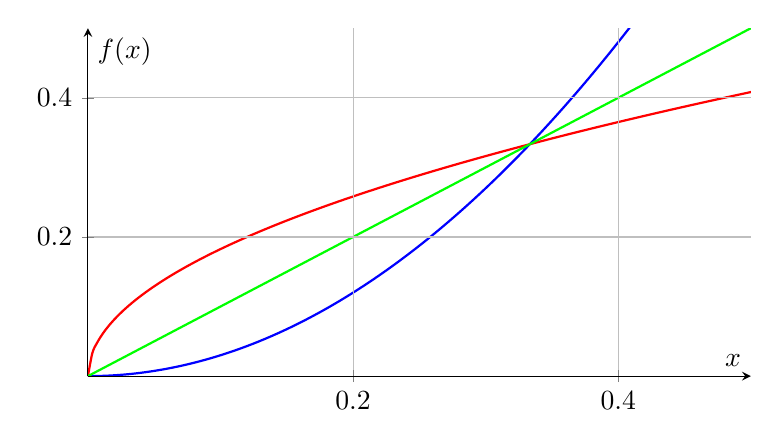
\begin{tikzpicture}
        \begin{axis}[
            axis lines = middle,
            xlabel = $x$, ylabel = {$f(x)$},
            xmin = 0, xmax = 0.5,
            ymin = 0, ymax = 0.5,
            xtick distance={0.2}, ytick distance={0.2},
            grid = both,
            width = 10cm,
            height = 6cm,
            samples = 10,
            smooth,
            axis on top,
        ]
        \addplot[blue, thick, domain=0:1, samples=300] {3*x^2};
        \addplot[red, thick, domain=0:1, samples=300] {sqrt(x / 3)};
        \addplot[green, thick, domain=0:1, samples=300] {x};
        \end{axis}
    \end{tikzpicture}
\end{center}
They are symmetrical along the line $y = x$ (green). Creating a table for each of these functions side by side reveals yet another property that inverse functions have.

Let's substitute $x = 3$ into $f$. That gives:
\begin{align*}
    f(3) &= 3(3)^2 \\
    &= 3(9) \\
    &= 27
\end{align*}
Now, let's plug this value into the inverse function $f^{-1}$.
\begin{align*}
    f^{-1}(3) &= \sqrt{\frac{27}{3}} \\
    &= \sqrt{9} \\
    &= 3
\end{align*}
Let's try the same for a different value, like $5$.
\begin{align*}
    f(5) &= 3(5)^2 & f^{-1}(75) &= \sqrt{\frac{75}{3}} \\
    &= 3(25) & &= \sqrt{25} \\
    &= 75 & &= 5
\end{align*}
What this means is: plugging the $y$-value of $f$ into $f^{-1}$ gives the $x$ value of $f$. A cleaner way of demonstrating this is by creating tables of each function side by side.
\begin{center}
    \begin{tabular}{ c | c }
        $x$ & $f(x) = 3x^2$ \\
        \hline
        $1$ & $3$ \\
        \hline
        $2$ & $12$ \\
        \hline
        $3$ & $27$
    \end{tabular}
    \quad
    \begin{tabular}{ c | c }
        $x$ & $f^{-1}(x) = \sqrt{\frac{x}{3}}$ \\
        \hline
        $3$ & $1$ \\
        \hline
        $12$ & $2$ \\
        \hline
        $27$ & $3$
    \end{tabular}
\end{center}
You may have noticed at this point that I haven't included the left side of the parabola. That's because the left side is \textbf{not} actually part of the inverse. The inverse function $f^{-1} = \sqrt{\frac{x}{3}}$ is a radical, meaning the result of $f^{-1}$ are valid. If I use negative $x$ values for $f$, I literally cannot swap the $x$ and $y$. The $x$ in $f(x)$ is being square, which negates any negative.
\begin{center}
    \begin{tabular}{ c | c }
        $x$ & $f(x) = 3x^2$ \\
        \hline
        $-1$ & $3$ \\
        \hline
        $-2$ & $12$ \\
        \hline
        $-3$ & $27$
    \end{tabular}
    \quad
    \begin{tabular}{ c | c }
        $x$ & $f^{-1}(x) = \sqrt{\frac{x}{3}}$ \\
        \hline
        $3$ & $1$ (not negative!!) \\
        \hline
        $12$ & $2$ (not negative!!)\\
        \hline
        $27$ & $3$ (not negative!!)
    \end{tabular}
\end{center}\clearpage
If I include the left side of the parabola in the graph I presented before, you can see why this is true.
\begin{figure}[ht]
    \caption{Parabola-Radical Example}
    \label{fig:Parabola-Radical Example}
    \centering
    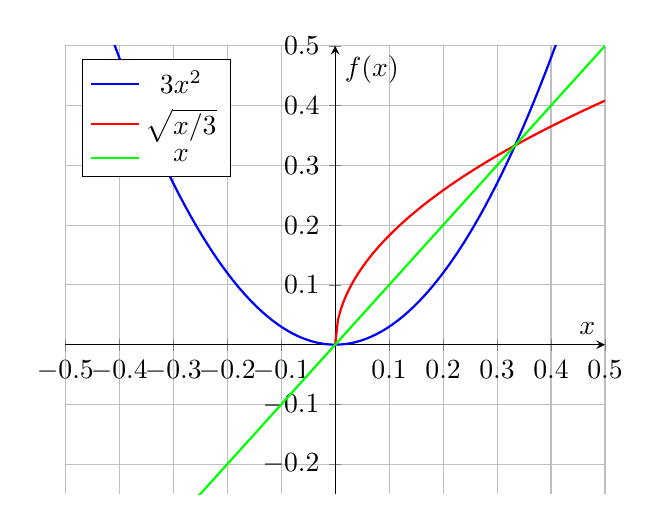
\begin{tikzpicture}
        \begin{axis}[
            axis lines = middle,
            xlabel = $x$, ylabel = {$f(x)$},
            xmin = -0.5, xmax = 0.5,
            ymin = -0.25, ymax = 0.5,
            xtick distance={0.1}, ytick distance={0.1},
            grid = both,
            legend pos = north west, % Positions the legend
        ]
            \addplot[blue, thick, domain=-0.5:0.5, samples=100] {3*x^2};
            \addlegendentry{$3x^2$}

            \addplot[red, thick, domain=0:0.5, samples=100] {sqrt(x / 3)};
            \addlegendentry{$\sqrt{x/3}$}

            \addplot[green, thick, domain=-0.5:0.5, samples=100] {x};
            \addlegendentry{$x$}
        \end{axis}
    \end{tikzpicture}
\end{figure}

The function $f^{-1}$ (red line) does not intersect $f$ (blue line) \textbf{or} $y = x$ (green line) when $x < 0$.

Let's formalize this with a definition.
\begin{definition}
    Given a function $f$, it's inverse $f^{-1}$ is such that
    \[
        f(f^{-1}) = x \text{ and } f^{-1}(f(x)) = x
    \]
    and the domain of $f$ is equal to the range of $f^{-1}$ (and vise versa).
\end{definition}
\clearpage
Before giving a problem for you to try on your own, I'll solve one more, slightly more difficult problem.

Given the function $f(x) = 3x^2 + 2x - 1$, find its inverse $f^{-1}$ and state its domain.

First, I'll rewrite it as an equation of $y$ and swap the variables
\begin{align*}
    y &= 3x^2 + 2x - 1 \\
    x &= 3y^2 + 2y - 1
\end{align*}
Now I'll solve for $y$.
\begin{align*}
    0 &= 3y^2 + 2x - 1 - x \\
    0 &= 3y^2 + 2x - (1 + x)
\end{align*}
I'll use the quadratic formula on the above equation with $a$, $b$, and $c$ defined like so
\[
\begin{aligned}
    a &= 3 \\
    b &= 2 \\
    c &= -(1 + x) = -x - 1
\end{aligned}
\]
The reason I'm using the quadratic formula is because we're given the standard form of a quadratic: $ax^2 + bx + c$. In the same way you'd solve for $x$ by using the quadratic formula, we can solve for $y$ using the quadratic formula. The solution for $y$ is as follows.
\begin{align*}
y &= \frac{-(2) \pm \sqrt{(2)^2 - 4(3)(-x - 1)}}{2(3)} && \text{Applied Quadratic Formula}\\
&= \frac{-2 \pm \sqrt{4 + 12(x + 1)}}{6} && \text{Simplified Radicand and Denominator}\\
&= \frac{-2 \pm \sqrt{4 + 12x + 12}}{6} && \text{Distributed $12$ Into The Parentheses}\\
&= \frac{-2 \pm \sqrt{12x + 16}}{6} && \text{Added Like Terms}\\
&= \frac{-2 \pm \sqrt{4(3x + 4)}}{6} && \text{Factored Out $4$ (the perfect square)}\\
&= \frac{-2 \pm 2\sqrt{3x + 4}}{6} && \text{Took $\sqrt{4} = 2$}\\
&= \frac{-1 \pm \sqrt{3x + 4}}{3} && \text{Divided Top and Bottom By $2$}
\end{align*}
\[
y = \frac{-1 \pm \sqrt{3x + 4}}{3} 
\]
In this case, we're only interested in the positive solution for $y$ for a few reasons:
\begin{enumerate}
    \item We want to ensure that the resulting expression is actually a function. Leaving it as $\pm$ turns the parabola sideways, which fails the vertical line test.
    \item The negative solution introduces a complication that I'll explain in just a moment.
\end{enumerate}
That leaves us with this inverse function as our solution.
\[
\boxed{f^{-1}(x) = \frac{\sqrt{3x + 4} - 1}{3}} \qquad \text{Swapped the terms in the numerator (optional)}
\]
Now for the domain. Although this \textit{is} a rational function, there are no variables in the denominator, so there is no restriction there. So the only limitation is the radical. We need to find the minimum value ($0$) of the radicand, so we can set it to $0$ and solve for $x$.
\begin{align*}
    3x + 4 &= 0 \\
    3x &= -4 \\
    x &= -\frac{4}{3}
\end{align*}
This means $x \ge -\frac{4}{3}$. Since this is the only restriction, we're done. To make it a bit more formal, we can write the domain restriction in interval notation like so: $x \in \left[-\frac{4}{3}, \infty \right)$.
\clearpage
Now. About that complication I was talking about... In our solution, we only cared about the positive solution. But you actually \textit{can} use the negative. The reason you're able to do that goes back to the example with the radical and parabola (see Figure \ref{fig:Parabola-Radical Example}).

To illustrate this, I'll create a graph for $f(x) = 3x^2 + 2x - 1$ and\\$f^{-1}(x) = \frac{\sqrt{3x + 4} - 1}{3}$. Notice how these are symmetric about the line $y = x$.
\vspace{-0.5cm}
\begin{figure}[ht]
    \centering
    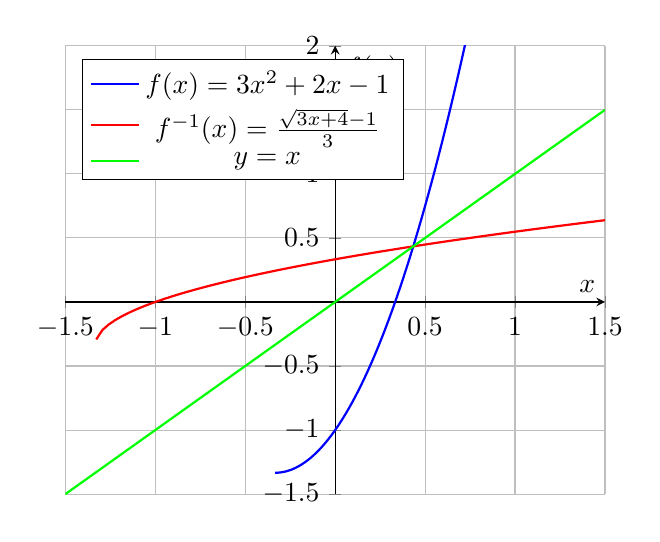
\begin{tikzpicture}
        \begin{axis}[
            axis lines = middle,
            xlabel = $x$, ylabel = {$f(x)$},
            xmin = -1.5, xmax = 1.5,
            ymin = -1.5, ymax = 2,
            xtick distance={0.5}, ytick distance={0.5},
            grid = both,
            legend pos = north west, % Positions the legend
        ]
            \addplot[blue, thick, domain=-0.33333:1.5, samples=100] {3 * x^2 + 2 * x - 1};
            \addlegendentry{$f(x) = 3x^{2}+2x-1$}

            \addplot[red, thick, domain=-2:1.5, samples=100] {(sqrt(3 * x + 4) - 1) / 3};
            \addlegendentry{$f^{-1}(x) = \frac{\sqrt{3x+4}-1}{3}$}

            \addplot[green, thick, domain=-2:1.5, samples=100] {x};
            \addlegendentry{$y = x$}
        \end{axis}
    \end{tikzpicture}
\end{figure}
\\
Now look at the graph for $f(x) = 3x^2 + 2x - 1$ and\\$f^{-1}(x) = \frac{-1 - \sqrt{3x + 4}}{3}$.
\vspace{-0.55cm}
\begin{figure}[ht]
    \centering
    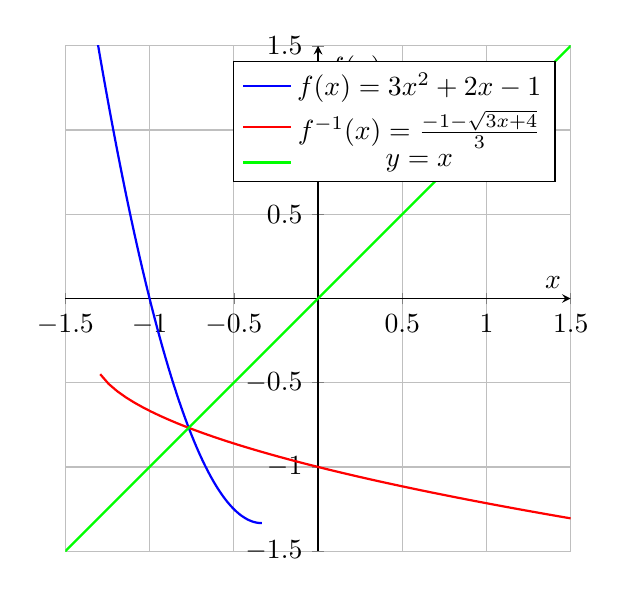
\begin{tikzpicture}
        \begin{axis}[
            axis lines = middle,
            xlabel = $x$, ylabel = {$f(x)$},
            xmin = -1.5, xmax = 1.5,
            ymin = -1.5, ymax = 1.5,
            xtick distance={0.5}, ytick distance={0.5},
            width = 8cm, height = 8cm,
            grid = both,
            legend pos = north east, % Positions the legend
        ]
            \addplot[blue, thick, domain=-2:-0.333333, samples=100] {3 * x^2 + 2 * x - 1};
            \addlegendentry{$f(x) = 3x^{2}+2x-1$}

            \addplot[red, thick, domain=-2:3, samples=100] {(-1 - sqrt(3 * x + 4)) / 3};
            \addlegendentry{$f^{-1}(x) = \frac{-1 - \sqrt{3x + 4}}{3}$}

            \addplot[green, thick, domain=-2:3, samples=100] {x};
            \addlegendentry{$y = x$}
        \end{axis}
    \end{tikzpicture}
\end{figure}
\\
Notice how these are also symmetric about the line $y = x$. The only difference is that the intersection is in the third quadrant instead of the first.
\clearpage
Although both are equally valid, the reason we take the positive solution is purely because of convention. Mathematicians came across this problem a while ago and had to decide which they wanted to normalize. They chose the positive solution as the convention, so that's what we use now.

I urge you to stick with the convention. Using the negative solution might not fare super well with your teacher (i.e. you may lose points for not choosing the positive).

As promised, I'll now give a probelm for you to try.
\begin{problem}
    Given the function $g(x) = \frac{3}{2x + 1}$, find the inverse function $g^{-1}$ and state its domain.
\end{problem}
\begin{solution}
    First, let's rewrite this function as an equation of $y$ in terms of $x$.
    \[
        y = \frac{3}{2x + 1}
    \]
    Next, let's swap the variables.
    \[
        x = \frac{3}{2y + 1}
    \]
    Now, let's solve for $y$.
    \begin{align*}
        x(2y + 1) &= 3 &&\text{Multiplied both sides by $2y + 1$} \\
        2y + 1 &= \frac{3}{x} && \text{Divided both sides by $x$} \\
        2y &= \frac{3}{x} - 1 && \text{Subtrated both sides by $1$} \\
        y &= \frac{\frac{3}{x} - 1}{2} && \text{Divided both sides by $2$}
    \end{align*}
    Since the denominator at the very bottom ($2$) doesn't have any variables, I can distribute it into the numerator. Doing so gives your inverse function.
    \[
        g^{-1}(x) = \frac{3}{2x} - \frac{1}{2}
    \]
    \clearpage
    Now to find the inverse. The only limitation here is the denominator $2x$. Since that denominator cannot equal $0$, we can set it equal to $0$ to see what value of $x$ would make the fraction invalid.
    \begin{align*}
        2x &= 0 \\
        x &= 0 && \text{Divided both sides by $2$}
    \end{align*}
    Although, we could've just noticed that anything times $0$ is $0$, meaning $2x = 0$ would simplify to $x = 0$, without doing any of that work. Since this is as simplified as it gets, we have our final answer:
    \[
        g^{-1}(x) = \frac{3}{2x} - \frac{1}{2} \text{ where } x \neq 0
    \]
\end{solution}
\clearpage\chapter{Piecewise Functions}
Piecewise functions are a kind of break from the composite and inverse functions we've been working on up to this point. Piecewise functions are best used when the formula deciding the input changes after a certain $x$ value. Examples often used with piecewise functions include tax brackets, shipment/delivery price changes, discounts dependent on age, etc.

Before hopping into any examples, I think it's best to get acquainted with what a piecewise function looks like and how to graph it. Consider the below piecewise function:
\[
f(x) = 
\begin{cases}
    x & 0 \le x \le 4 \\
    -(x - 4) + 4 & 4 < x \le 8 \\
    \frac{x - 8}{2} & x > 8
\end{cases}
\]
What do you think this looks like? I've written the explanation of this on the next page, so take a moment to think about what happens before moving on.
\begin{itemize}
    \item Why are there compound inequalities next to equations?
    \item Why are some of the inequalities $<$ and others $\le$?
    \item What's up with that $x > 8$ in the bottom row? Why is it different?
    \item Could these compound inequalities by written in some other way?
\end{itemize}
\clearpage
\section{Describing Piecewise Functions}
Alright. Here it is.

The $f(x)$ is the name of the function, as is the case with any other function. It is set equal to a curly bracket containing cases.

Each row first identifies and equation and next by an interval that the equation applies within.

Using the above function as an example:
\[
x \qquad \qquad 0 \le x \le 4
\]
means to say that the equation $y = x$ applies for all $x$ values between $0$ and $4$.
\[
-(x - 4) + 4 \qquad \qquad 4 < x \le 8
\]
means to say that the equation $y = -(x - 4) + 4$ applies for all $x$ values between $4$ and $8$ excluding $4$. The value $x = 4$ is excluded because it's already accounted for in the previous domain.
\[
\frac{x - 8}{2} \qquad \qquad x > 8
\]
means to say that the equation $\frac{x - 8}{2}$ applies for all $x$ values that are greater than $8$. Again, the inequality is not $x \ge 8$ because the value $x = 8$ was accounted for in the previous domain.

The inequality $x > 8$ could be written as $8 < x < \infty$ so that it matches the other inequalities.

The piecewise function could also be rewritten using interval notation, like so:
\[
f(x) = 
\begin{cases}
    x & x \in [0, 4]\\
    -(x - 4) + 4 & x \in (4, 8] \\
    \frac{x - 8}{2} & x \in (8, \infty)
\end{cases}
\]
\clearpage
This piecewise function produces the graph below:
\begin{figure}[ht]
    \centering
    \caption{Graph Of Piecewise Function $f(x)$}
    \label{fig:Piecewise Example 1}
    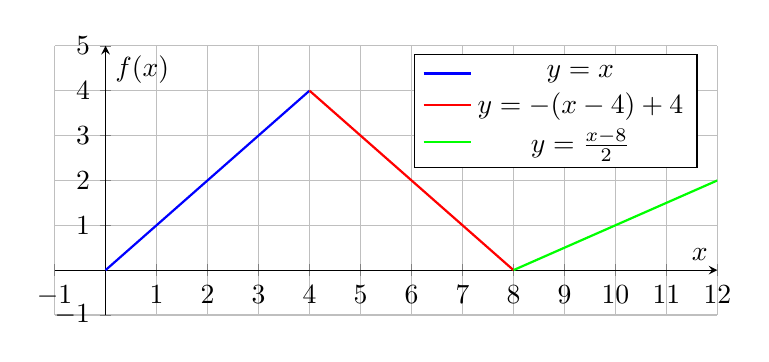
\begin{tikzpicture}
        \begin{axis}[
            axis lines = middle,
            xlabel = $x$, ylabel = {$f(x)$},
            xmin = -1, xmax = 12,
            ymin = -1, ymax = 5,
            xtick distance={1}, ytick distance={1},
            width = 10cm, height = 5cm,
            grid = both,
            legend pos = north east, % Positions the legend
        ]
            \addplot[blue, thick, domain=0:4, samples=100] {x};
            \addlegendentry{$y = x$}

            \addplot[red, thick, domain=4:8, samples=100] {-(x - 4) + 4};
            \addlegendentry{$y = -(x - 4) + 4$}

            \addplot[green, thick, domain=8:12, samples=100] {(x - 8) / 2};
            \addlegendentry{$y = \frac{x - 8}{2}$}
        \end{axis}
    \end{tikzpicture}
\end{figure}
\section{Example with Piecewise Functions}
Now that we know what a piecewise function \textit{is}, let's look at an example of where it may be used.

"Totally real bank name" gives money out for free. If we say that $x$ represents the number of hours that have passed, then:
\begin{itemize}
    \item The first $4$ hours, represented as $0 \le x \le 4$, \$$10$ are given out per hour.
    \item The following $9$ hours, represented as $4 < x \le 13$, \$$7$ are given per hour.
    \item Every hour after that, represented as $x > 13$ or $13 < x < \infty$, \$$5$ are given out per hour.
\end{itemize}
Instead of writing each and every case, we can use a piecewise function to set all three cases equal to a function $f$. This function will output the amount of money given out after $x$ hours.
\clearpage
\subsection{Potential Trap}
We should be careful when constructing such a function, however. We can't simply call the equatoins $10x$, $7x$ and $5x$. 
\begin{align*}
f(x) &= 
\begin{cases}
    10x & x \in [0, 4]\\
    7x & x \in (4, 13] \\
    5x & x \in (13, \infty)
\end{cases}
&& \longleftarrow \text{Bad Piecewise Function}
\end{align*}
Doing so creates the piecewise function above and graph in Figure \ref{fig:Bad Piecewise Example 1} below.
\begin{figure}[ht]
    \centering
    \caption{Piecewise Function with Incorrect Equations}
    \label{fig:Bad Piecewise Example 1}
    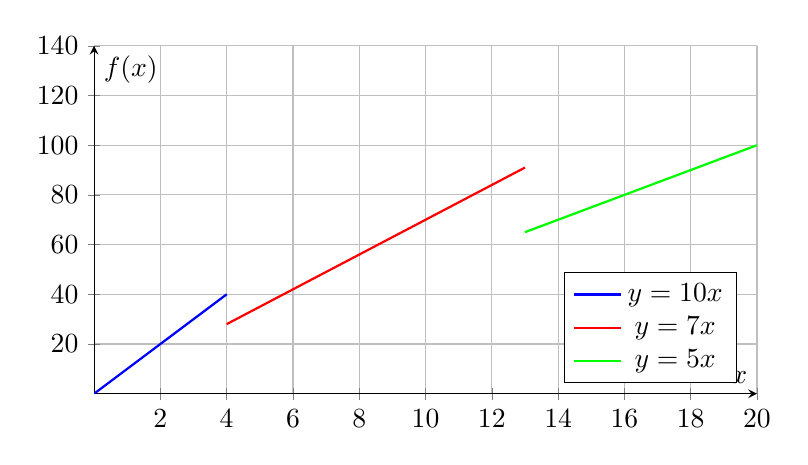
\begin{tikzpicture}
        \begin{axis}[
            axis lines = middle,
            xlabel = $x$, ylabel = {$f(x)$},
            xmin = 0, xmax = 20,
            ymin = 0, ymax = 140,
            xtick distance={2}, ytick distance={20},
            width = 10cm, height = 6cm,
            grid = both,
            legend pos = south east, % Positions the legend
        ]
            \addplot[blue, thick, domain=0:4, samples=100] {10 *x};
            \addlegendentry{$y = 10x$}

            \addplot[red, thick, domain=4:13, samples=100] {7 * x};
            \addlegendentry{$y = 7x$}

            \addplot[green, thick, domain=13:20, samples=100] {5 * x};
            \addlegendentry{$y = 5x$}
        \end{axis}
    \end{tikzpicture}
\end{figure}
\\
Just throwing these into a piecewise function would create a valid function, but one that doesn't represent the situation given. For it to represent the provided situation, the lines need to be connected. Let's examine why.

If $4$ hours passed, and $10$ dollars were given out every hour, then $40$ dollars were given out.

When the fifth hour passes, the piecewise function moves to the next equation, which we've currently assigned as $7x$. Plugging $x = 5$ to $7x$ gives $7 \times 5 = 35$. That's $5$ dollars less than what was given out in the first $4$ hours.

Since the amount given out in the fifth hour must add to the amount already given on the first $4$, we expect the amount after $5$ hours (i.e. $f(5)$) to be $47$ dollars.
\clearpage
You may think, "just shift the function up $12$ units ($y = 7x + 12$). Doing that gets us up to the $47$ we expect ($35 + 12 = 47$)." Although this \textit{would} work, it requires that you know how much was given out at the fourth hour.

Of course you can do that in this example. It's easy. But something like the one below would not be very easy to determine:
\begin{itemize}
    \item $\sin\left(\pi x\right)+\tan\left(\frac{x}{2}\right)$ acts on $x \in \left[-\frac{\pi}{13}, \frac{\pi}{9} \right]$
    \item $\tan\left(\frac{\pi^{2}x}{22}\right)$ acts on $x \in \left(\frac{\pi}{9}, \frac{\pi}{2}\right]$
\end{itemize}
The solution to that looks like this if you're curious:
\[
g(x) = 
\begin{cases}
    \sin\left(\pi x\right)+\tan\left(\frac{x}{2}\right) & 
    x \in \left[-\frac{\pi}{13}, \frac{\pi}{9} \right] \\
    %
    \tan\left(\frac{\pi^{2}\left(x-\frac{\pi}{9}\right)}{22}\right)+\sin\left(\frac{\pi^{2}}{9}\right)+\tan\left(\frac{\pi}{18}\right) & 
    x \in \left(\frac{\pi}{9}, \frac{\pi}{2}\right]
\end{cases}
\]
\vspace{-0.5cm}
\begin{figure}[ht]
    \centering
    \caption{Super Hard Problem (Scale: $\frac{\pi}{8}$)}
    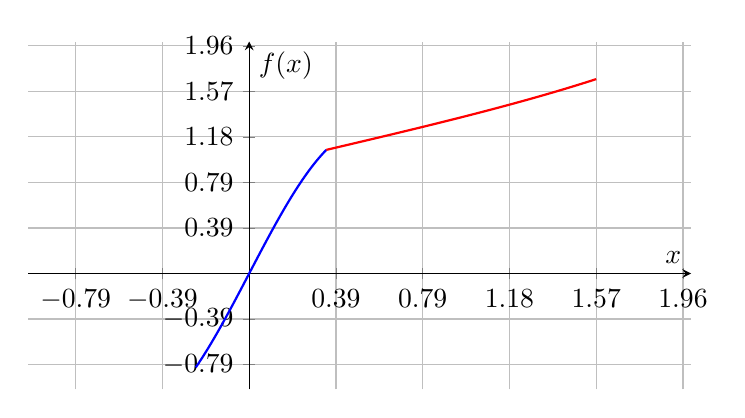
\begin{tikzpicture}
        \begin{axis}[
            axis lines = middle,
            xlabel = $x$, ylabel = {$f(x)$},
            xmin = -1, xmax = 2,
            ymin = -1, ymax = 2,
            xtick distance={pi / 8}, ytick distance={pi / 8},
            width = 10cm, height = 6cm,
            grid = both,
            legend pos = north east, % Positions the legend
            trig format plots=rad
        ]
            \addplot[blue, thick, domain=-(pi / 13):(pi / 9), samples=100] {sin(pi * x) + tan(x / 2)};
            \addplot[red, thick, domain=(pi / 9):(pi / 2), samples=100] {tan((pi^2 * (x - (pi / 9))) / 22) + sin(pi^2 / 9) + tan(pi / 18)};
        \end{axis}
    \end{tikzpicture}
\end{figure}
\clearpage
\subsection{The Correct Way To Do It}
Let's go back to the problem we were working on.

Instead of predicting or calculating how much we should add or subtract, we can literally move the entire function using vertical and horizontal transformations. 

In this case, we know that $y = 10x$ up until $x = 4$.

We're already given that $x = 4$, and $10 \times 4 = 40$, meaning $y = 40$.

What's left is to apply those transformations ($4$ right and $40$ up) to $7x$.

That gives: $y = 7(x - 4) + 40$.

This method does not rely on any calculations. All you need is the right-most edge of the bound ($4$ in this case) and the value of the equation at that bound ($40$ in this case). The same can be done for the last function.

In the first $4$ hours, the bank gave out $40$ dollars. In the next $9$ hours, the bank gave out $7 \times 9 = 63$ dollars. That means the total amount given is $40 + 63 = 103$ dollars.

We also know that the right-most boundary of the second equation is $x = 13$. That means we need to transform $5x$ 13 units to the right and $103$ units up, giving $y = 5(x - 13) + 103$.

Putting that all together gives the piecewise function and graph below:
\begin{center}
    \raisebox{0.5cm}{%
        \begin{minipage}[c]{0.48\textwidth}
            \centering
            \[
            g(x) = 
            \begin{cases}
                10x & x \in [0, 4] \\
                7(x - 4) + 40 & x \in (4, 13] \\
                5(x - 13) + 103 & x \in (13, \infty)
            \end{cases}
            \]
        \end{minipage}%
    }
    \begin{minipage}[c]{0.48\textwidth}
        \centering
        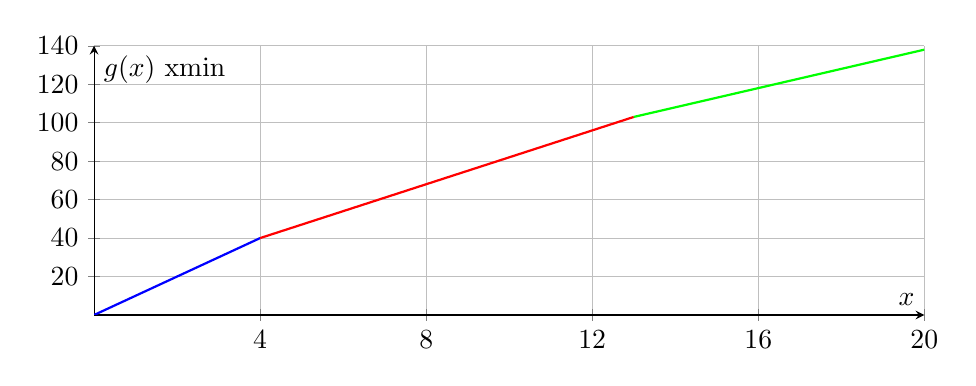
\begin{tikzpicture}
            \begin{axis}[
                axis lines = middle,
                xlabel = $x$, ylabel = {$g(x)$}
                xmin = 0, xmax = 20,
                ymin = 0, ymax = 140,
                xtick distance={4}, ytick distance={20},
                width = \linewidth,   % scale to the minipage width
                height = 5cm,
                grid = both,
                legend pos = south east,
            ]
                \addplot[blue, thick, domain=0:4, samples=100] {10 * x};
                \addplot[red, thick, domain=4:13, samples=100] {7 * (x - 4) + 40};
                \addplot[green, thick, domain=13:20, samples=100] {5 * (x - 13) + 103};
            \end{axis}
        \end{tikzpicture}
    \end{minipage}
\end{center}
\clearpage
\section{Jump Discontinuity}
Up to this point, we've been working with functions that continue cleanly from one another. To illustrate this point, I'll use another example. For those of you also taking physics, this sort of example may look familiar:
\begin{problem}
    Janet is a frequent runner and takes the same route to her friend's house every day. On her daily runs, she:
    \begin{itemize}
        \item Runs $1000\,m$ in $30$ minutes.
        \item Rests for $5$ minutes.
        \item Runs $750\,m$ in $30$ minutes.
        \item Rests for $10$ minutes.
        \item Runs $1200\,m$ in $45$ minutes.
    \end{itemize}
    Create a piecewise function and a Velocity vs. Time graph (VT Graph) representing Janet's velocity.
\end{problem}
For those who haven't taken physics, a Velocity vs. Time graph is just like a normal function but the $x$-axis is time $t$ and the $y$-axis is velocity $v$.

Also, instead of using $f(x)$ or $g(x)$, I'll be using $v(t)$, a velocity function with time (in minutes) as the independent variable.

We're not given any velocities, but we can find them quickly. Velocity is calculated by dividing the distance traveled by the time it took to travel that distance. For example, if you drove $30$ miles in $2$ hours then you were going $30\,mi / 2\,hr = 15\,mi/hr$. 

Using the equation $v = \frac{\Delta s}{\Delta t}$ ($s$ stands for change in position btw), we get:
\begin{align*}
    v_1 &= \frac{1000}{30} &
    v_2 &= \frac{0}{5} &
    v_3 &= \frac{750}{30} &
    v_4 &= \frac{0}{10} & 
    v_5 &= \frac{1200}{45} \\
    %
    v_1 &= \frac{100}{3} &
    v_2 &= 0 &
    v_3 &= 25 &
    v_4 &= 0 &
    v_5 &= \frac{80}{3}
\end{align*}
\clearpage
We don't have any variables here, so there's nothing to line up. That means we can create the piecewise function and graph right now:
\begin{center}
    \begin{minipage}[c]{0.48\linewidth}
        \[
            v(t) = 
            \begin{cases}
            \frac{100}{3} & t \in [0, 30] \\
            0 & t \in (30, 35] \\
            25 & t \in (35, 65] \\
            0 & t \in (65, 75] \\
            \frac{80}{3} & t \in (75, 120]
            \end{cases}
        \]
    \end{minipage}
    \begin{minipage}[c]{0.48\textwidth}
        \centering
        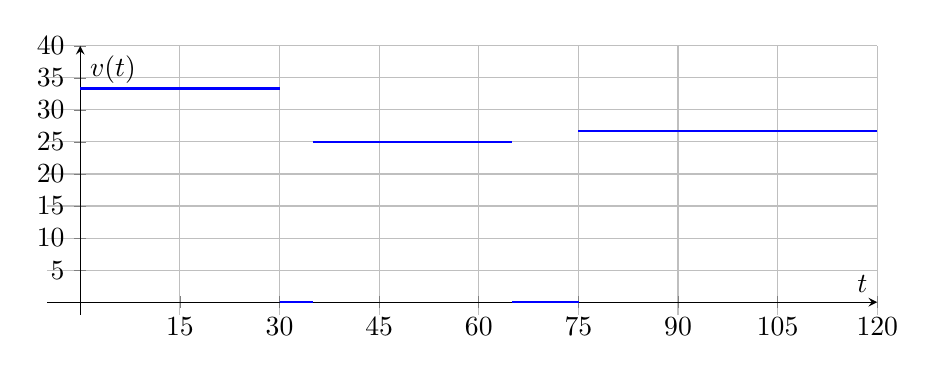
\begin{tikzpicture}
            \begin{axis}[
                axis lines = middle,
                xlabel = $t$, ylabel = {$v(t)$},
                xmin = -5, xmax = 120,
                ymin = -2, ymax = 40,
                xtick distance={15}, ytick distance={5},
                width = \linewidth,   % scale to the minipage width
                height = 5cm,
                grid = both,
                legend pos = south east,
            ]
                \addplot[blue, thick, domain=0:30, samples=100] {100 / 3};
                \addplot[blue, thick, domain=30:35, samples=100] {0};
                \addplot[blue, thick, domain=35:65, samples=100] {25};
                \addplot[blue, thick, domain=65:75, samples=100] {0};
                \addplot[blue, thick, domain=75:120, samples=100] {80 / 3};
            \end{axis}
        \end{tikzpicture}
    \end{minipage}
\end{center}
This function doesn't smoothly transition like with the bank example. It breaks off and continues in different places. It jumps from $v = 35$ all the way down to $v = 0$, hence why it's called a "jump" discontinuity. This is \textbf{not} continuous. Also... $25$ minutes per minute? Dayum she's slow. But that's beside the point.
\clearpage
\section{Removable Discontinuity}
A removable discontinuity is a less obvious than a jump discontinuity. The function may \textit{look} continuous, but it'll have a hole somewhere. I won't spend too much time on this because it's solved almost identically to regular piecewise functions. In fact, I can actually use a previous example to demonstrate this.

Here was the result from that bank example:
\begin{center}
    \raisebox{0.5cm}{%
        \begin{minipage}[c]{0.48\textwidth}
            \centering
            \[
            g(x) = 
            \begin{cases}
                10x & x \in [0, 4] \\
                7(x - 4) + 40 & x \in (4, 13] \\
                5(x - 13) + 103 & x \in (13, \infty)
            \end{cases}
            \]
        \end{minipage}%
    }
    \begin{minipage}[c]{0.48\textwidth}
        \centering
        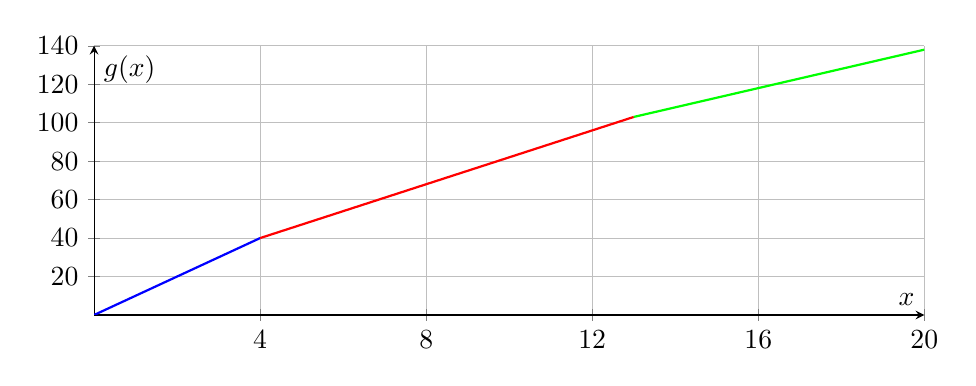
\begin{tikzpicture}
            \begin{axis}[
                axis lines = middle,
                xlabel = $x$, ylabel = {$g(x)$},
                xmin = 0, xmax = 20,
                ymin = 0, ymax = 140,
                xtick distance={4}, ytick distance={20},
                width = \linewidth,   % scale to the minipage width
                height = 5cm,
                grid = both,
                legend pos = south east,
            ]
                \addplot[blue, thick, domain=0:4, samples=100] {10 * x};
                \addplot[red, thick, domain=4:13, samples=100] {7 * (x - 4) + 40};
                \addplot[green, thick, domain=13:20, samples=100] {5 * (x - 13) + 103};
            \end{axis}
        \end{tikzpicture}
    \end{minipage}
\end{center}
This function is continuous because there are no gaps. But what if we changed the inequality $x \in [0, 4]$ to $x \in [0, 4)$?

If we did that, the function would begin at $0$, continue all the way up to $3.99999\dots$, then skip $4$ to go to $4.00000\dots 1$ and continue as normal. Making some substitutions would help visualize what's going on.
\begin{align*}
    f(3.9) &= 39 \\
    f(4) &= undefined \\
    f(4.1) &= 40.7
\end{align*}
\clearpage
Since the function has nothing defined for $x = 4$ (i.e. it's skipped), it's labeled as undefined. The function $f$ has no value at $x = 4$. On a graph, that is usually labeled by an open circle.

With that change, the piecewise function and graph now looks like this:
\begin{center}
    \raisebox{0.5cm}{%
        \begin{minipage}[c]{0.48\textwidth}
            \centering
            \[
            g(x) = 
            \begin{cases}
                10x & x \in [0, 4) \\
                7(x - 4) + 40 & x \in (4, 13] \\
                5(x - 13) + 103 & x \in (13, \infty)
            \end{cases}
            \]
        \end{minipage}%
    }
    \begin{minipage}[c]{0.48\textwidth}
        \centering
        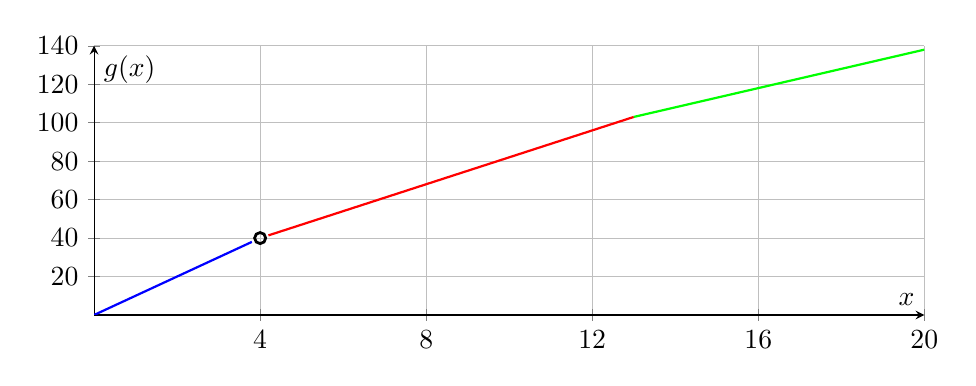
\begin{tikzpicture}
            \begin{axis}[
                axis lines = middle,
                xlabel = $x$, ylabel = {$g(x)$},
                xmin = 0, xmax = 20,
                ymin = 0, ymax = 140,
                xtick distance={4}, ytick distance={20},
                width = \linewidth,   % scale to the minipage width
                height = 5cm,
                grid = both,
                legend pos = south east,
            ]
                \addplot[blue, thick, domain=0:3.8, samples=100] {10 * x};
                \addplot[red, thick, domain=4.2:13, samples=100] {7 * (x - 4) + 40};
                \addplot[green, thick, domain=13:20, samples=100] {5 * (x - 13) + 103};
                \addplot[only marks, mark=o, mark options={draw=black, fill=white, line width=1pt}, mark size=2pt] coordinates {(4, 40)};
            \end{axis}
        \end{tikzpicture}
    \end{minipage}
\end{center}
\clearpage
\part{Trigonometry}
Congratulations. If you've made it up to this point, you should be comfortable (or somewhat comfortable) with functions. What you learned in the Functions part will carry to \textbf{all} future classes, math or not.

However important functions are, trigonometry is what I'd consider the \textit{heart} of pre-calculus. This goes beyond what you may or may not have covered in your Algebra II or Integrated III class. Here, we're diving into trigonometric functions, identities, the unit circle, inverse trig functions, applications of these functions, and more. I'll detail below what I'll be covering as a reference.
\section*{Chapter Overview}
In no particular order:
\begin{itemize}
    \item Degrees vs. Radians 
    \item The Unit Circle
    \item Basic trigonometric functions and their properties (sine, cosine, tangent)
    \item Transformations of Trigonometric Functions
    \item Reciporicals of the basic functions (secant, cosecant, cotangent)
    \item Inverse trigonometric functions
    \item Various identities (some with derivations)
\end{itemize}
I know, I know. Another laundry list of things to cover after just having gone through functions. But not to worry! A good portion of what you'll learn here are extensions of the Funtions part. Be sure to take things lightly. Don't let the math intimidate. It \textit{is} new, but no more difficult than anything else covered.

Once again, I'll do my best to break things down, highlighting any pitfalls and traps that may come your way.

With that said, good luck to you! You're gonna have fun!
\clearpage\chapter{Radians And Degrees}
Radians. It's that pesky settings on your calculator your teacher cautions you about in class or before a test.

Up to this point, you've used degrees for everything.
\begin{itemize}
    \item All angles of triangles or intersetions between lines are in \textit{degrees}.
    \item We all learn that a right angle is exactly $90$ \textit{degrees}.
    \item We're given that a circle is $360$ \textit{degrees}.
    \item And so on...
\end{itemize}
However, as you continue moving forward in math, you'll gradually step away from degrees and use radians almost exclusively. In fact, the moment you're taught what radians are is when the switch happens. Degrees still have their place but, in my experience up to Calculus III, it's pretty much never used.

So what \textit{are} radians anyway? Like degrees, radians measure angles. But it's measured in a very specific way. For simplisity sake, I'll use the $xy$-plane to demonstrate.
\clearpage
\section{Getting Measurements}
All angle measurements begin from the positive $x$-direction, meaning the positive $x$-direction is $0$ radians. The angle increases in size as you rotate counter-clockwise. 

For example, if you wanted to get to $45$ degrees, you would begin from the positive $x$-direction (or the positive $x$-axis), and create a $45\degree$ angle between the $x$-axis and a line starting at the origin. It would look something like this:

% Text Area is 12 cm wide.
\begin{minipage}[c]{0.33\linewidth}
    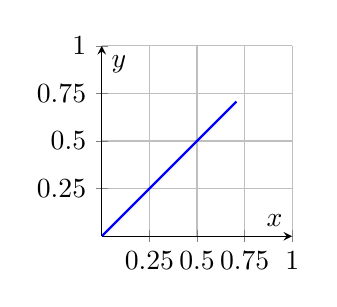
\begin{tikzpicture}
        \begin{axis}[
            axis lines = middle,
            xlabel = $x$, ylabel = {$y$},
            xmin = 0, xmax = 1,
            ymin = 0, ymax = 1,
            xtick distance={0.25}, ytick distance={0.25},
            width = 4cm,   % scale to the minipage width
            height = 4cm,
            grid = both,
            legend pos = south east,
        ]
            \addplot[blue, thick, domain=0:sqrt(2)/2, samples=100] {x};
        \end{axis}
    \end{tikzpicture}
\end{minipage}
\begin{minipage}[c]{0.66\linewidth}
    From the figure, we can see that the angle formed by the blue line and the positive $x$-axis is $45$ degrees. This also happens to be \textit{exactly} the line $y = x$. We'll get into why as we move further into the text.
\end{minipage}

If we wanted $90$ degrees, the line would instead point vertically in the positive $y$-direction like so:
\begin{center}
    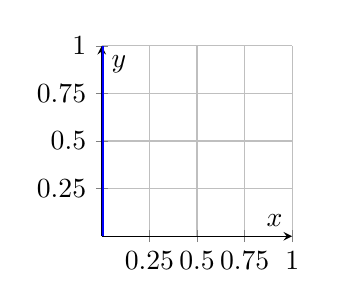
\begin{tikzpicture}
        \begin{axis}[
            axis lines = middle,
            xlabel = $x$, ylabel = {$y$},
            xmin = 0, xmax = 1,
            ymin = 0, ymax = 1,
            xtick distance={0.25}, ytick distance={0.25},
            width = 4cm,   % scale to the minipage width
            height = 4cm,
            grid = both,
            legend pos = south east,
        ]
            \draw[ultra thick, blue] (0,0) -- (0,1);
        \end{axis}
    \end{tikzpicture}
\end{center}
\clearpage
\section{Radian As A Unit Of Measurement}
Now to discuss what exactly a radian is.

The measurement is derived from arc lengths starting from the positive $x$-direction of a circle with a radius of $r = 1$, also known as the \textbf{unit circle} ("unit" signifies the $1$ unit radius of the circle).

Try thinking about it this way:

Place a circle with radius $1$ at to origin, such that it's center is at $(0,0)$. That should look something like the figure below.
\begin{center}
    \begin{minipage}[c]{0.33\linewidth}
        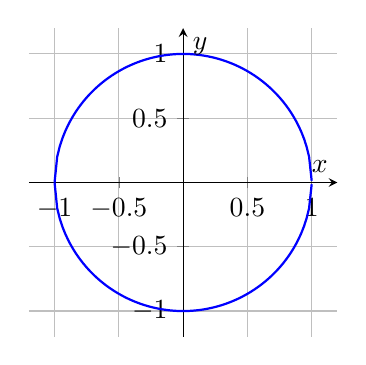
\begin{tikzpicture}
            \begin{axis}[
                axis lines = middle,
                xlabel = $x$, ylabel = {$y$},
                xmin = -1.2, xmax = 1.2,
                ymin = -1.2, ymax = 1.2,
                xtick distance={0.5}, ytick distance={0.5},
                width = 5.5cm,
                height = 5.5cm,
                grid = both,
                legend pos = south east,
            ]
                \addplot[blue, thick, domain=-1:1, samples=100] {sqrt(1 - x^2)};
                \addplot[blue, thick, domain=-1:1, samples=100] {-1 * sqrt(1 - x^2)};
            \end{axis}
        \end{tikzpicture}
    \end{minipage}
    \begin{minipage}[c]{0.66\linewidth}
        The equation for the circumference, $C$, of a circle is
        \[
            C = 2\pi r \text{.}
        \]
        Because we're working with a circle that has a radius of $r = 1$, we have:
        \[
            C = 2\pi \text{.}
        \]
    \end{minipage}
\end{center}
This means, if you start from the positive $x$ direction, move counter-clockwise around the entire circle, and eventually return to the positive $x$ direction, you'll have traveled $2\pi$ radians.

Now, suppose you wanted to draw a line that starts from the center of the circle at $(0,0)$ and ends at the perimeter of the circle. 

For the purposes of understanding radians, assume the line you drew starts at $(0,0)$ and ends at $(0,1)$ (that's straight up from the origin). We'll call this line $L$. 

The angle, in radians, formed by the line $L$ and the positive $x$-axis is the length of the arc that starts from the positive $x$-axis to the point where $L$ touches the circle.
\begin{center}
    \begin{minipage}[c]{0.33\linewidth}
        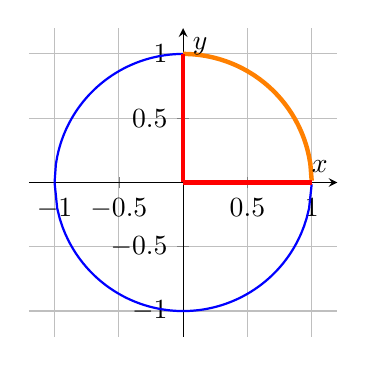
\begin{tikzpicture}
            \begin{axis}[
                axis lines = middle,
                xlabel = $x$, ylabel = {$y$},
                xmin = -1.2, xmax = 1.2,
                ymin = -1.2, ymax = 1.2,
                xtick distance={0.5}, ytick distance={0.5},
                width = 5.5cm,
                height = 5.5cm,
                grid = both,
                legend pos = south east,
            ]
                \addplot[blue, thick, domain=-1:0, samples=100] {sqrt(1 - x^2)};
                \addplot[blue, thick, domain=-1:1, samples=100] {-1 * sqrt(1 - x^2)};
                % %
                \addplot[orange, ultra thick, domain=0:1, samples=100] {sqrt(1 - x^2)}; %Arc length
                \addplot[red, ultra thick, domain=0:1, samples=10] {0};
                \draw[red, ultra thick] (0,0) -- (0,1); %Line from origin to (0,1)
            \end{axis}
        \end{tikzpicture}
    \end{minipage}
    \begin{minipage}[c]{0.66\linewidth}
        Denoted in red are:
        \begin{itemize}
            \item The vertical line, $L$, drawn from the origin.
            \item The positive $x$-axis that is within the circle.
        \end{itemize}
        Denoted in orange is the arc created from the positive $x$-axis to where the vertical line touches the circle.
    \end{minipage}
\end{center}
Notice that this arc is one-fourth of the circumference of the circle.

We've already established that the entire circumference of the circle is $2\pi$. Therefore, we can say that the length of the orange arc is $\frac{\pi}{2}$.

With that, we've now found that the angle formed by the two red lines creates an angle that is $\frac{\pi}{2}$ radians.

Rest assured that you \textbf{do not} have to find the length of an arc on the unit circle every time you want to find angles in radians. In fact, for the foreseeable future, you don't have to find any angles at all.

The example above only serves to demonstrate what exactly a measurement in radians is supposed to mean.
\clearpage
\subsection{Why a Radius of 1?}
Using a radius of $1$ makes the math so much easier. It:
\begin{enumerate}
    \item Removes the radius from the circumference equation $C = 2\pi$.
    \item Exponentially simplifies the trigonometric identities you'll learn later in this part.
    
    For example, the Pythagorean Identity with $r = 1$ is $\sin^2(\theta) + \cos^2(\theta) = 1$ (beautiful). If you used $r = 0.5$, you'd have $\sin^2(\theta) + \cos^2(\theta) = 0.25$ (that's ugly). With $r = 1$, you get $1^2 = 1$. With $r = 0.5$, you get $0.5^2 = 0.25$.
    \item It simplifies differentiation and integration (topics you'll be introduced to in Calculus I and expanded upon in Calculus II and III).
    
    For example, if you used $r = 2$ with Trigonometric Substitution (covered in Calculus II), you could no longer easily use the following:
    \begin{itemize}
        \item For $\sqrt{a^2 - x^2}$, use $x = a\sin(\theta)$
        \item For $\sqrt{a^2 + x^2}$, use $x = a\tan(\theta)$
        \item For $\sqrt{x^2 - a^2}$, use $x = a\sec(\theta)$
    \end{itemize}
    The above are built on the idea that $r = 1$. Changing that would require you, and the entire mathemematics community, to rethink how they work.
\end{enumerate}
These are only three of the \textbf{many} things that rely on $r = 1$, some of which go beyond what \textit{I} know. Long story short, stick with $r = 1$. It's the sweet spot that makes everything much, \textbf{much} easier.
\clearpage
\section{Converting Between Degrees and Radians}
Now you'll learn how to convert between degrees and radians.

The formulas are as follows:
\begin{itemize}
    \item Radians to Degrees $rad \times \frac{180}{\pi}$.
    \item Degress to Radians $deg \times \frac{\pi}{180}$.
\end{itemize}
To understand why this works, let's look at the unit circle again.
\begin{center}
    \begin{minipage}[t]{0.35\textwidth}
        \centering
        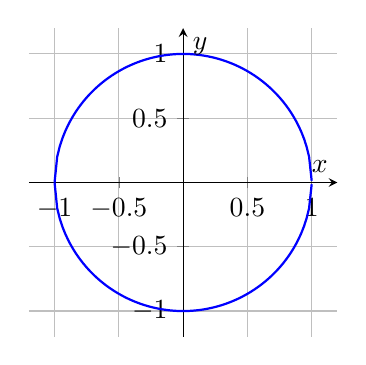
\begin{tikzpicture}[baseline=(current bounding box.north)]
            \begin{axis}[
                axis lines = middle,
                xlabel = $x$, ylabel = {$y$},
                xmin = -1.2, xmax = 1.2,
                ymin = -1.2, ymax = 1.2,
                xtick distance={0.5}, ytick distance={0.5},
                width = 5.5cm,
                height = 5.5cm,
                grid = both,
                legend pos = south east,
            ]
                \addplot[blue, thick, domain=-1:1, samples=100] {sqrt(1 - x^2)};
                \addplot[blue, thick, domain=-1:1, samples=100] {-1 * sqrt(1 - x^2)};
            \end{axis}
        \end{tikzpicture}
    \end{minipage}%    <-- % important to avoid a space
    \begin{minipage}[t]{0.64\textwidth}
        A circle has $360 \degree$. That is, if we start in the positive $x$ direction and traveled around the circle until we ended where we started, we would've traveled a full $360\degree$ around the circle. 
        \\ \\
        Knowing what we know about radians, we could also say that travling around the circle menas we did a full $2\pi$ radians around the circle.
    \end{minipage}
\end{center}
With this in mind, we can agree that $360\degree = 2\pi\,rad$. So, technically, $\frac{360}{2\pi} = 1$.

Conversely, $\frac{2\pi}{360} = 1$ also.

Simplifying both of these gives:
\begin{align*}
    \frac{360}{2\pi} = 1 &\Longrightarrow \frac{180}{\pi} = 1 \\
    \frac{2\pi}{360} = 1 &\Longrightarrow \frac{\pi}{180} = 1
\end{align*}
When converting, because the numerator is the same as the denominator, multiplying a value by this factor doesn't change it.

For example, if we had $\frac{\pi}{2}$ radians and we wanted to convert this to degrees, we'd multiply it by $\frac{180}{\pi}$.
\begin{align*}
    \frac{\pi}{2}\,rad  \cdot \frac{180}{\pi} &= \frac{180\pi}{2\pi} = 90\degree \\
\end{align*}
It's easy to forget which equation you should when converting. Here's how I remember it.
\begin{itemize}
    \item If an angle in radians is equal to that same measurement in degrees, the actual number in radians is \textit{always} smaller (i.e. $2\pi$, which is approximately $6.28$, is \textit{much} smaller than $360$). If we actually divide $\frac{\pi}{180}$, we get approximately $0.017453$, which is a really smaller number.
    
    Anything $\times$ Number less than $1$ $=$ Smaller Number.

    So, when converting from degrees to radians, we want to use $\frac{\pi}{180}$.

    \item Likewise, if an angle in radians is equal to an angle in degrees, the value in degrees is \textit{always} greater (i.e. $360$ is a lot bigger than $2\pi \approx 6.28$). If we divide $\frac{180}{\pi}$, we get approximately $57.29578$, which is pretty big.
    
    Anything $\times$ Number greater than $1$ $=$ Bigger Number.

    So, when converting from radians to degrees, we want to use $\frac{180}{\pi}$.
\end{itemize}
Let's try a few conversions together.
\begin{problem}
    Convert $45$ degrees to radians.
\end{problem}
\begin{solution}
    Since we're converting \textit{from} degrees \textit{to} radians, we need to use $\frac{\pi}{180}$.
    \begin{align*}
        45 \cdot \frac{\pi}{180} &= \frac{45\pi}{180}\\
        &= \frac{\pi}{4} && 45 \cdot 4 = 90 \cdot 2 = 180
    \end{align*}
\end{solution}
\clearpage
\begin{problem}
    Convert $\frac{\pi}{6}$ radians to degrees.
\end{problem}
\begin{solution}
    This time, we're converting \textit{from} radians \textit{to} degrees. So we need to use $\frac{180}{\pi}$.
    \begin{align*}
        \frac{\pi}{6} \cdot \frac{180}{\pi} &= \frac{180\pi}{6\pi} \\
        &= 30
    \end{align*}
\end{solution}
Let's do one last one just to make sure you're paying attention.
\begin{problem}
    Convert $1.5708$ radians to degrees.
\end{problem}
\begin{solution}
    Once again, we're converting from radians to degrees. So we must use $\frac{180}{\pi}$.
    \[
        1.5708 \cdot \frac{180}{\pi} = \frac{180(1.5708)}{\pi}
    \]
    This evaluates to roughly $90.00021\degree$. This value is almost $90\degree$. That's because $1.5708$ is approximately $\frac{\pi}{2}$, and $\frac{\pi}{2}$ is equal to $90\degree$.
\end{solution}
\clearpage\chapter{Basic Trigonometric Functions}
Like any other function, trigonometric functions can take inputs, produce outputs, be used to create a graph, transform/translate, etc. However, trigonometric functions are different in that they require additional vocabulary and properties to discuss.

The basic functions you'll learn in this chapter are the sine, cosine, and tangent functions. These three are the SOH-CAH-TOA you may have learned back in geometry. You'll be using them a \textit{lot} more here in pre-calculus and in all future calculus courses.

Let's start with sine.
\clearpage
\section{The Sine Function}
The sine function is one of the three basic trigonometric functions. It takes angles (either in degrees or radians) as an input and outputs the ratio of the side opposite the angle and hypotenuse of a right triangle. This is written as:
\begin{center}
    \begin{minipage}[c]{0.4\linewidth}
        \centering
        \begin{tikzpicture}
            \begin{axis}[%
                xmin = -0.3, xmax = 1.1,
                ymin = -0.3, ymax = 1.1,
                axis lines = none, % Hidden axes make the triangle pop more
                width = \linewidth, height = \linewidth
            ]
            % The Sides
            \draw[blue, thick] (0,0) -- (1,0) node[midway, below, black] {adj};
            \draw[red, thick] (1,0) -- (0,1) node[midway, above right, black] {hyp};
            \draw[red, thick] (0,0) -- (0,1) node[midway, left, black] {opp};
            
            % The Angle Theta
            \node[right] at (0.65, 0.1) {$\theta$};
            \draw[color = black, thick] (0.8,0) arc (180:135:0.2);
            
            % Right angle symbol
            \draw[thick, color = black] (0,0.1) -- (0.1,0.1) -- (0.1,0);
            \end{axis}
        \end{tikzpicture}
    \end{minipage}%
    \begin{minipage}[c]{0.2\linewidth}
        \[
            \sin(\theta) = \frac{\text{opposite}}{\text{hypotenuse}}
        \]
    \end{minipage}
\end{center}

However, the sine function is more than just its definition. Let's dive deeper into what the sine function is.
\begin{center}
    \begin{minipage}[c]{0.33\linewidth}
        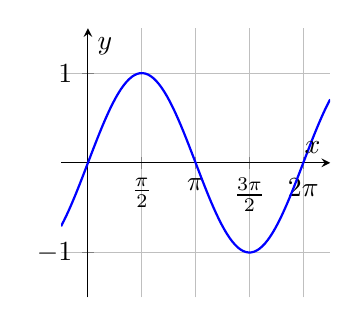
\begin{tikzpicture}
            \begin{axis}[%
                xlabel = {$x$}, ylabel = {$y$},
                xmin = -1 * 0.25 * pi, xmax = (9 * pi) / 4,
                ymin = -1.5, ymax = 1.5,
                xtick = {
                    0, 
                    pi / 2, 
                    pi, 
                    (3 * pi) / 2,
                    2 * pi%
                    },
                xticklabels = {
                    $0$,
                    $\frac{\pi}{2}$,
                    $\pi$,
                    $\frac{3\pi}{2}$,
                    $2\pi$%
                },
                ytick = {
                    -1,
                    1
                },
                axis lines = center, grid = both,
                width = 5cm, height = 5cm,
                trig format plots=rad
            ]
            \addplot[color = blue, thick, domain = -1 * 0.25 * pi:9/4*pi, samples = 100]{sin(x)};
            \end{axis}
        \end{tikzpicture}
    \end{minipage}
    \begin{minipage}[c]{0.66\textwidth}
        At left is the function $f(x) = \sin(x)$ graphed on the $xy$-plane, where $x$ is an angle in radians. There are a few things to note about this function.
        \begin{itemize}
            \item It's not like any function we've seen in the past. It's a wave that goes up and down as it moves along $x$.
            \item It has \textbf{zeroes} at $0$, $\pi$, and $2\pi$. More generally, it has zeroes at $n\pi$, where $n$ is any integer\\
            (i.e. $1,2,3,4,\text{etc.}$)
        \end{itemize}
    \end{minipage}
\end{center}
\begin{itemize}
    \item It has a maximum and minimum value of $1$ and $-1$, meaning the range of this function is $y \in [-1, 1]$. (yet another reason why $r = 1$ is so important).
    \begin{itemize}
        \item Those peaks are reached when $x = \frac{\pi(2n + 1)}{2}$, where $n$ is an integer\\(i.e. $1,2,3,4,\text{etc.}$) This ensures that the numerator is $\frac{\text{odd number} \times \pi}{2}$. Using $2n + 1$ (which guarantees an odd number) is what gets the values 
        $x = \frac{1\pi}{2}, \frac{3\pi}{2}, \frac{5\pi}{2},\dots$
    \end{itemize}
    \item At $x = 2\pi$, it essentially resets to what it was at $x = 0$ (same direction and $y$-value).
    \item It may not look super obvious from the table, but this function continues forever in the positive and negative $x$ directions. This means the domain of $\sin(x)$ is $x \in (-\infty, \infty)$.
\end{itemize}
\clearpage
\section{The Cosine Function}
The cosine function is very similar to the sine function. It's the second of the three basic trigonometric functions. Like the sine function, it takes angles (either in degrees or radians) as an input. But it instead outputs the ratio of the side adjacent to the angle and hypotenuse of a right triangle. This is written as:

\begin{center}
    \begin{minipage}[c]{0.4\linewidth}
        \centering
        \begin{tikzpicture}
            \begin{axis}[%
                xmin = -0.3, xmax = 1.1,
                ymin = -0.3, ymax = 1.1,
                axis lines = none,
                width = \linewidth, height = \linewidth
            ]
            
            \draw[red, thick] (0,0) -- (1,0) node[midway, below, black] {adj};
            \draw[red, thick] (1,0) -- (0,1) node[midway, above right, black] {hyp};
            \draw[blue, thick] (0,0) -- (0,1) node[midway, left, black] {opp};
            
            \node[right] at (0.65, 0.1) {$\theta$};
            \draw[color = black, thick] (0.8,0) arc (180:135:0.2);
            
            \draw[thick, color = black] (0,0.1) -- (0.1,0.1) -- (0.1,0);
            \end{axis}
        \end{tikzpicture}
    \end{minipage}%
    \begin{minipage}[c]{0.3\linewidth}
        \[
            \cos(\theta) = \frac{\text{adjacent}}{\text{hypotenuse}}
        \]
    \end{minipage}
\end{center}
\begin{center}
    \begin{minipage}[c]{0.33\linewidth}
        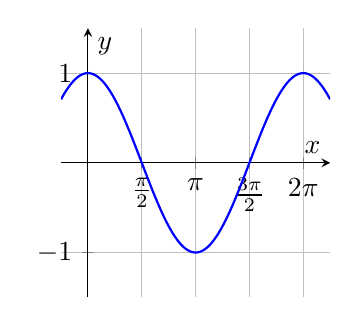
\begin{tikzpicture}
            \begin{axis}[%
                xlabel = {$x$}, ylabel = {$y$},
                xmin = -1 * 0.25 * pi,, xmax = (9 * pi) / 4,
                ymin = -1.5, ymax = 1.5,
                xtick = {
                    0, 
                    pi / 2, 
                    pi, 
                    (3 * pi) / 2,
                    2 * pi%
                    },
                xticklabels = {
                    $0$,
                    $\frac{\pi}{2}$,
                    $\pi$,
                    $\frac{3\pi}{2}$,
                    $2\pi$%
                },
                ytick = {
                    -1,
                    1
                },
                axis lines = center, grid = both,
                width = 5cm, height = 5cm,
                trig format plots=rad
            ]
            \addplot[color = blue, thick, domain = -1 * 0.25 * pi:9/4*pi, samples = 100]{cos(x)};
            \end{axis}
        \end{tikzpicture}
    \end{minipage}
    \begin{minipage}[c]{0.66\textwidth}
        At left is the function $f(x) = \cos(x)$ graphed on the $xy$-plane, where $x$ is an angle in radians. There are a few things to note about this function.
        \begin{itemize}
            \item Like the sine function, it's a wave that goes up and down as it moves along $x$.
            \item It has \textbf{zeroes} at $\frac{\pi}{2}$ and $\frac{3\pi}{2}$. More generally, it has zeroes at $\frac{\pi(2n + 1)}{2}$, where $n$ is any odd integer\\
            (i.e. $1,3,5,7,\text{etc.}$)
        \end{itemize}
    \end{minipage}
\end{center}
\begin{itemize}
    \item It has a maximum and minimum value of $1$ and $-1$, meaning the range of this function is $y \in [-1, 1]$. (yet another reason why $r = 1$ is so important).
    \begin{itemize}
        \item Those peaks are reached when $x = n\pi$, where $n$ is an integer\\(i.e. $1,2,3,4,\text{etc.}$)
    \end{itemize}
    \item Just like the sine function, it essentially resets to what it was at $x = 0$ when it reaches $x = 2\pi$ (same direction and $y$-value).
    \item Also like the sine function, it continues forever in the positive and negative $x$ directions. This means the domain of $\cos(x)$ is $x \in (-\infty, \infty)$.
\end{itemize}
Something you may notice about the cosine function is that it is exactly equal to the sine function if you move it $\frac{\pi}{2}$ units to the right. In other words:
\begin{align*}
    \text{In Radians: } &\sin(\theta) = \cos\left(\theta - \frac{\pi}{2} \right) \\
    \text{In Degrees: } &\sin(\theta) = \cos\left(\theta - 90\right)
\end{align*}
\clearpage
\section{The Tangent Function}
The tangent is a bit different than the sine and cosine. It \textit{is} a basic trigonometric function, and \textit{is} defined by sides of a right triangle, it does not follow the same up and down wave pattern.

The tangent of an angle is defined as the ratio of the opposite and adjacent sides of a right triangle. It is also expressed as the sine function divided by the cosine function.
\begin{center}
    \begin{minipage}[c]{0.4\linewidth}
        \centering
        \begin{tikzpicture}
            \begin{axis}[%
                xmin = -0.3, xmax = 1.1,
                ymin = -0.3, ymax = 1.1,
                axis lines = none,
                width = \linewidth, height = \linewidth
            ]
            
            \draw[red, thick] (0,0) -- (1,0) node[midway, below, black] {adj};
            \draw[blue, thick] (1,0) -- (0,1) node[midway, above right, black] {hyp};
            \draw[red, thick] (0,0) -- (0,1) node[midway, left, black] {opp};
            
            \node[right] at (0.65, 0.1) {$\theta$};
            \draw[color = black, thick] (0.8,0) arc (180:135:0.2);
            
            \draw[thick, color = black] (0,0.1) -- (0.1,0.1) -- (0.1,0);
            \end{axis}
        \end{tikzpicture}
    \end{minipage}%
    \begin{minipage}[c]{0.3\linewidth}
        \begin{align*}
            \tan(\theta) &= \frac{opposite}{adjacent} \\
            \tan(\theta) &= \frac{\sin(\theta)}{\cos(\theta)}
        \end{align*}
    \end{minipage}
\end{center}
Let's look at the graph of the tangent function, but it's quite different from the sine and cosine.
\begin{center}
    \begin{minipage}[c]{0.33\linewidth}
        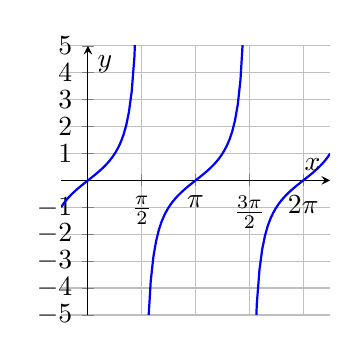
\begin{tikzpicture}
            \begin{axis}[%
                xlabel = {$x$}, ylabel = {$y$},
                xmin = -1 * 0.25 * pi,, xmax = (9 * pi) / 4,
                ymin = -5, ymax = 5,
                restrict y to domain=-10:10,
                xtick = {
                    0, 
                    pi / 2, 
                    pi, 
                    (3 * pi) / 2,
                    2 * pi%
                    },
                xticklabels = {
                    $0$,
                    $\frac{\pi}{2}$,
                    $\pi$,
                    $\frac{3\pi}{2}$,
                    $2\pi$%
                },
                ytick = {
                    -5,
                    -4,
                    -3,
                    -2,
                    -1,
                    1,
                    2,
                    3,
                    4,
                    5%
                },
                axis lines = center, grid = both,
                width = 5cm, height = 5cm,
                trig format plots=rad
            ]
            \addplot[color = blue, thick, domain = -1 * 0.25 * pi:9/4*pi, samples = 100]{tan(x)};
            \end{axis}
        \end{tikzpicture}
    \end{minipage}
    \begin{minipage}[c]{0.66\textwidth}
        At left is $f(x) = \tan(x)$ graphed on the $xy$-plane, where $x$ is an angle in radians. There are some things to note about this function.
        \begin{itemize}
            \item Unlike the sine and cosine functions, there are asymptotes in this function. They appear when $x = \frac{\pi(2n + 1)}{2}$, where $n$ is an integer (i.e. $1,2,3,4,\text{etc.}$)
        \end{itemize}
    \end{minipage}
\end{center}
The notation $\frac{\pi(2n + 1)}{2}$ indicates that the numerator is always $\pi$ multiplied by an odd number. These values include:
\begin{align*}
    n = 1&: \frac{\pi}{2} \\
    n = 2&: \frac{3\pi}{2} \\
    n = 3&: \frac{5\pi}{2} \\
    n = a&: \frac{\pi(2a + 1)}{2} && \text{$a$ is an arbitrarily large integer}
\end{align*}
We could also say that $n$ is an odd integer (i.e. $1,3,5,7,\text{etc.}$) like we did in the cosine section.

To understand why, remember that the tangent function is defined as the sine function divided by the cosine function. That means $\cos(x)$ is in the denominator.

From the section on the cosine function, we know that $\cos(x)$ has zeroes when $x = \frac{\pi(2n + 1)}{2}$. As a result, tangent is not continuous/undefined at those values of $x$.

As for why the function shoots up to infinity when it gets close to those $x$ values, recall what happened when we plugged smaller and smaller values into the function $g(x) = \frac{1}{x}$ back when we first covered asymptotes. The smaller the denominator got, the large the output got. For example:
\begin{align*}
    g(0.000000001) &= \frac{1}{0.000000001} = 1000000000 \\
    g(-0.000000001) &= -\frac{1}{0.000000001} = -1000000000
\end{align*}
The same is happeneing in this function. As the angle (in radians) gets closer to, say, $\frac{\pi}{2}$, $\sin(x)$ gets closer and closer to $1$ and $\cos(x)$ gets closer and closer to $0$. When this happens, what we get is something like this:
\begin{align*}
    \tan\left(\frac{\pi}{2} - 0.0001 \right) &= \frac{\sin\left(\frac{\pi}{2} - 0.0001 \right)}{\cos\left(\frac{\pi}{2} - 0.0001 \right)}
    \approx \frac{0.9999999999}{0.00001} \approx 99999.999\dots \\
    \tan\left(\frac{\pi}{2} + 0.0001 \right) &= \frac{\sin\left(\frac{\pi}{2} + 0.0001 \right)}{\cos\left(\frac{\pi}{2} + 0.0001 \right)}
    \approx \frac{0.9999999999}{-0.00001} \approx -99999.999\dots
\end{align*}
\begin{itemize}
    \item Tangent has zeroes at $x = n\pi$, where $n$ is an integer (i.e. $1,2,3,4,\text{etc.}$)
\end{itemize}
This is true for the same reason as the previous. In the definition of the tangent function, $\sin(x)$ is in the numerator. From the sine section, we learned that $\sin(x) = 0$ when $x = n\pi$, so $\frac{0}{anything} = 0$.
\clearpage
With everything we have, we can say the following about the domain and range:
\begin{align*}
    x \neq \frac{\pi(2n + 1)}{2} \\
    y \in (-\infty, \infty)
\end{align*}
Or, if we wanna get fancy, we can use:
\[
    \text{Domain}: \left\{ x \mid x \neq \frac{\pi(2n + 1)}{2}, n \in \mathbb{Z} \right\} \\
\]
This is called \textbf{set-builder} notation. It just means that $x$ cannot equal $\frac{\pi(2n + 1)}{2}$ where $n$ is an integer. $\mathbb{Z}$ is the set of all integers. So if $n$ is in the set of all integers, then it's also an integer. 

But don't worry about that notation. I never saw set-builder notation in Calculus II and, while I \textit{have} seen it in Calculus III, I've never had to write one myself. Your teacher/professor will not expect you to know this, and you probably won't touch it for a \textit{while}. It's pretty cool to know, though.
\clearpage
\chapter{Properties of Trigonometric Functions}
I had originally written the section on the properties of trigonometric functions as part of the "Basic Trigonometric Functions" chapter, but it got \textit{really} long. Long enough that I eventually decided to make it it's own chapter.

I'll begin with the period and then continue to frequency.
\section{Period For The Sine and Cosine Functions}
The period of a function is how long it takes to complete one full cycle, where one full cycle is how long it takes for the function to reset. 

In the sine and cosine sections, we learned that the functions "essentially reset" when reaching $x = 2\pi$. With this, we know that the period of $\sin(x)$ and $\cos(x)$ is $2\pi$.

To clarify, take a look at the functions again.
\begin{center}
    \begin{minipage}[c]{0.45\linewidth}
        \begin{tikzpicture}
            \begin{axis}[%
                title = {$f(x) = \sin(x)$},
                xlabel = {$x$}, ylabel = {$y$},
                xmin = -1 * 0.25 * pi, xmax = (9 * pi) / 4,
                ymin = -1.5, ymax = 1.5,
                xtick = {
                    0, 
                    pi / 2, 
                    pi, 
                    (3 * pi) / 2,
                    2 * pi%
                    },
                xticklabels = {
                    $0$,
                    $\frac{\pi}{2}$,
                    $\pi$,
                    $\frac{3\pi}{2}$,
                    $2\pi$%
                },
                ytick = {
                    -1,
                    1
                },
                axis lines = center, grid = both,
                width = \linewidth, height = \linewidth,
                trig format plots=rad
            ]
            \addplot[color = blue, thick, domain = -1 * 0.25 * pi:9/4*pi, samples = 100]{sin(x)};
            \end{axis}
        \end{tikzpicture}
    \end{minipage}
    \hspace{0.05\linewidth}
    \begin{minipage}[c]{0.45\linewidth}
                \begin{tikzpicture}
            \begin{axis}[%
                title = {$f(x) = \cos(x)$},
                xlabel = {$x$}, ylabel = {$y$},
                xmin = -1 * 0.25 * pi, xmax = (9 * pi) / 4,
                ymin = -1.5, ymax = 1.5,
                xtick = {
                    0, 
                    pi / 2, 
                    pi, 
                    (3 * pi) / 2,
                    2 * pi%
                    },
                xticklabels = {
                    $0$,
                    $\frac{\pi}{2}$,
                    $\pi$,
                    $\frac{3\pi}{2}$,
                    $2\pi$%
                },
                ytick = {
                    -1,
                    1
                },
                axis lines = center, grid = both,
                width = \linewidth, height = \linewidth,
                trig format plots=rad
            ]
            \addplot[color = blue, thick, domain = -1 * 0.25 * pi:9/4*pi, samples = 100]{cos(x)};
            \end{axis}
        \end{tikzpicture}
    \end{minipage}
\end{center}
For the sine function, it begins at $(0,0)$ and moves up on the $xy$-plane. Then, when it reaches $x = 2\pi$, it returns to a height of $y = 0$ and is pointing up again, just as it did at $(0,0)$. Since it returns to its original state at $x = 2\pi$, it has a period of $2\pi$.

For the cosine function, it begins at $(0,1)$ and moves down on the $xy$-plane. Then, when it reaches $x = 2\pi$, it returns to a height of $y = 1$ and is pointing down again, just as it did at $(0,1)$. Since it returns to its original state at $x = 2\pi$, it has a period of $2\pi$.
\clearpage
Now let's try squishing the graph. I'll get into how you can do that in the transformation section, so don't worry about that. Just look at the graphs.
\begin{center}
    \begin{minipage}[c]{0.45\linewidth}
        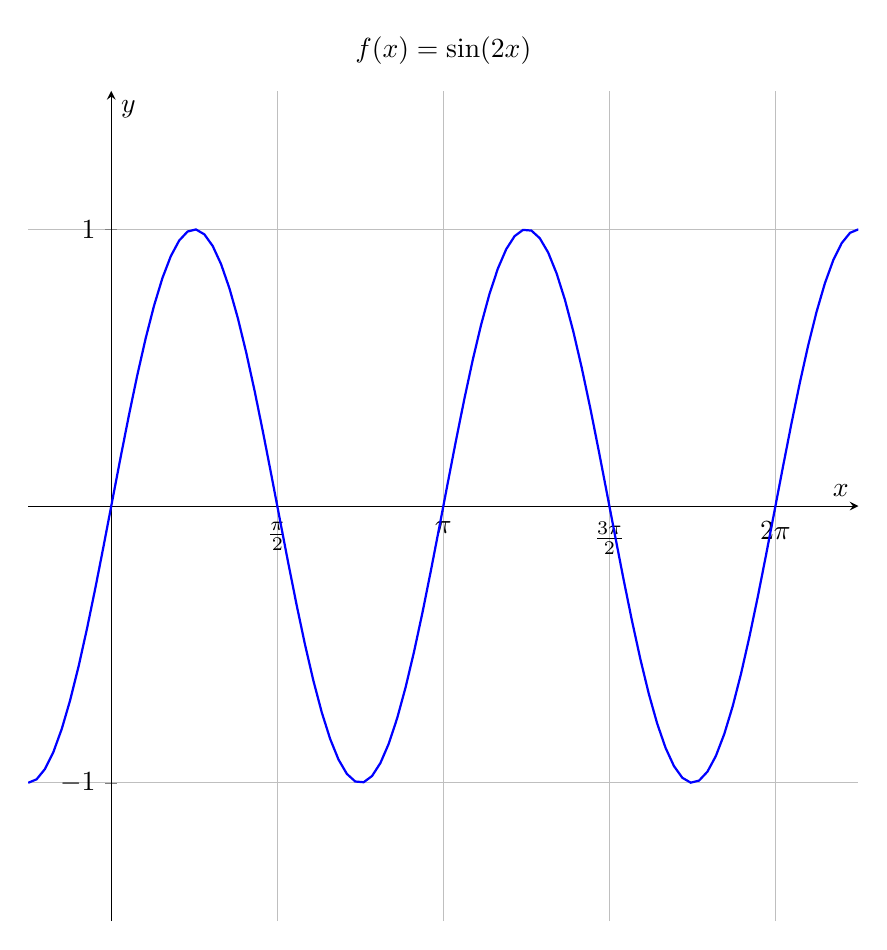
\begin{tikzpicture}
            \begin{axis}[%
                title = {$f(x) = \sin(2x)$},
                xlabel = {$x$}, ylabel = {$y$},
                xmin = -1 * 0.25 * pi, xmax = (9 * pi) / 4,
                ymin = -1.5, ymax = 1.5,
                xtick = {
                    0, 
                    pi / 2, 
                    pi, 
                    (3 * pi) / 2,
                    2 * pi%
                    },
                xticklabels = {
                    $0$,
                    $\frac{\pi}{2}$,
                    $\pi$,
                    $\frac{3\pi}{2}$,
                    $2\pi$%
                },
                ytick = {
                    -1,
                    1
                },
                axis lines = center, grid = both,
                width = \linewidth, height = \linewidth,
                trig format plots=rad
            ]
            \addplot[color = blue, thick, domain = -1 * 0.25 * pi:9/4*pi, samples = 100]{sin(2 * x)};
            \end{axis}
        \end{tikzpicture}
    \end{minipage}
    \hspace{0.05\linewidth}
    \begin{minipage}[c]{0.45\linewidth}
                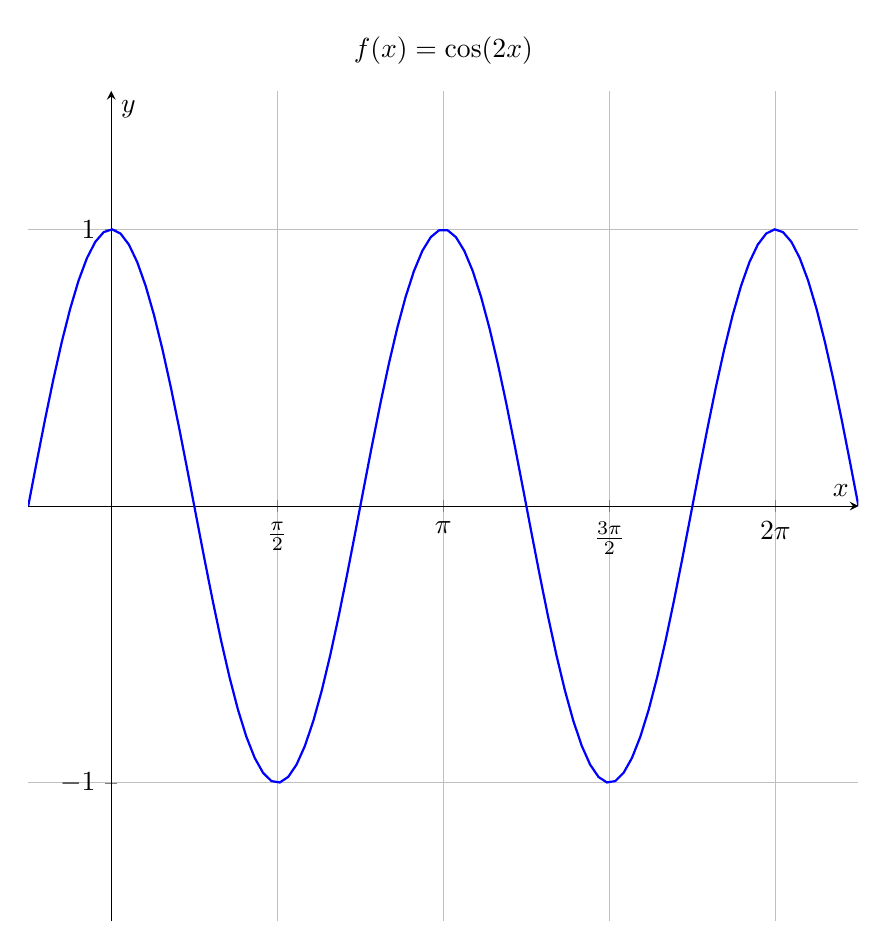
\begin{tikzpicture}
            \begin{axis}[%
                title = {$f(x) = \cos(2x)$},
                xlabel = {$x$}, ylabel = {$y$},
                xmin = -1 * 0.25 * pi, xmax = (9 * pi) / 4,
                ymin = -1.5, ymax = 1.5,
                xtick = {
                    0, 
                    pi / 2, 
                    pi, 
                    (3 * pi) / 2,
                    2 * pi%
                    },
                xticklabels = {
                    $0$,
                    $\frac{\pi}{2}$,
                    $\pi$,
                    $\frac{3\pi}{2}$,
                    $2\pi$%
                },
                ytick = {
                    -1,
                    1
                },
                axis lines = center, grid = both,
                width = \linewidth, height = \linewidth,
                trig format plots=rad
            ]
            \addplot[color = blue, thick, domain = -1 * 0.25 * pi:9/4*pi, samples = 100]{cos(2 * x)};
            \end{axis}
        \end{tikzpicture}
    \end{minipage}
\end{center}
The sine function, once again, begins at $(0,0)$ and points up. However, notice what's happeneing. There seems to be an extra wave. 

The function still points up and has a height of $y = 0$ at $x = 2\pi$, but it's \textbf{not the first occurance of it}. The first time it happens is actually at $x = \pi$.

For that reason, the frequency of $\sin(2x)$ is $\pi$ instead of $2\pi$.

The same applies for the cosine function. It begins at $(0,1)$ and points down. It has a height of $y = 1$ and also points down at at $x = 2\pi$, but it's \textbf{not the first occurance}.

Like the sine function, it reaches its first reset at $x = \pi$. Therefore, it also has a period of $\pi$.

Give this next one a shot. Before I reveal the answer on the next page, try determining the period yourself.
\begin{center}
    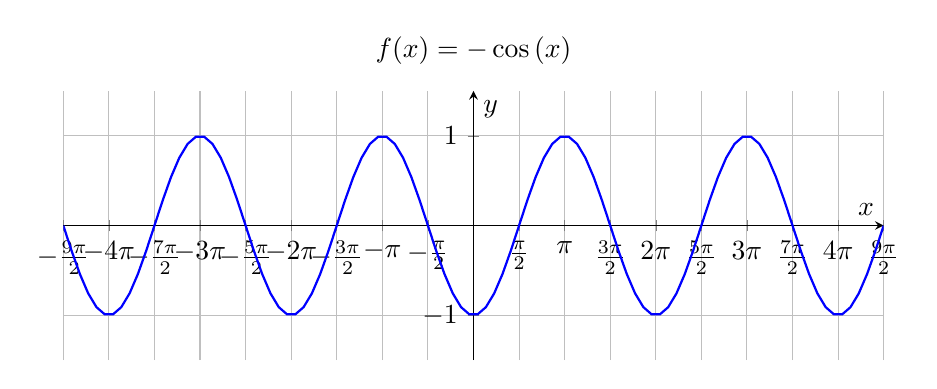
\begin{tikzpicture}
        \begin{axis}[%
            title = {$f(x) = -\cos\left(x\right)$},
            xlabel = {$x$}, ylabel = {$y$},
            xmin = -1 * (9 / 2) * pi, xmax = (9 / 2) * pi,
            ymin = -1.5, ymax = 1.5,
            xtick = {
                -1 * (9 * pi) / 2,
                -1 * 4 * pi,
                -1 * (7 * pi) / 2,
                -1 * 3 * pi,
                -1 * (5 * pi) / 2,
                -1 * 2 * pi,
                -1 * (3 * pi) / 2,
                -1 * pi,
                -1 * pi / 2,
                0, 
                pi / 2, 
                pi, 
                (3 * pi) / 2,
                2 * pi,
                (5 * pi) / 2,
                3 * pi,
                (7 * pi) / 2,
                4 * pi,
                (9 * pi) / 2%
                },
            xticklabels = {
                $-\frac{9\pi}{2}$,
                $-4\pi$,
                $-\frac{7\pi}{2}$,
                $-3\pi$,
                $-\frac{5\pi}{2}$,
                $-2\pi$,
                $-\frac{3\pi}{2}$,
                $-\pi$,
                $-\frac{\pi}{2}$,
                $0$,
                $\frac{\pi}{2}$,
                $\pi$,
                $\frac{3\pi}{2}$,
                $2\pi$,
                $\frac{5\pi}{2}$,
                $3\pi$,
                $\frac{7\pi}{2}$,
                $4\pi$,
                $\frac{9\pi}{2}$%
            },
            ytick = {
                -1,
                1
            },
            axis lines = center, grid = both,
            width = 12cm, height = 5cm,
            trig format plots=rad
        ]
        \addplot[color = blue, thick, domain = {-1 * (9 * pi) / 2}:{(9 / 2) * pi}, samples = 100]{-1 * cos(x)};
        \end{axis}
    \end{tikzpicture}
\end{center}
This one's a bit more challenging, but the answer here is $2\pi$.

Looking at the graph, we see that it begins at $(0, -1)$ and is moving up when $x = 0$. That means we need to look for the first instance where the function returns to a height of $y = -1$ and points up. That first instance happens at $x = 2\pi$. See below for the comparrison between $x = 0$ and $x = 2\pi$.
\begin{center}
    \begin{minipage}[c]{0.45\linewidth}
        \begin{tikzpicture}
            \begin{axis}[%
                title = {$f(x) = -\cos(x)$ when $x = 0$},
                xlabel = {$x$}, ylabel = {$y$},
                xmin = -1 * 0.5 * pi, xmax = 0.5 * pi,
                ymin = -1.5, ymax = 1.5,
                xtick = {
                    -1 * 0.5 * pi,
                    -1 * 0.25 * pi,
                    0,
                    0.25 * pi,
                    0.5 * pi
                    },
                xticklabels = {
                    $-\frac{\pi}{2}$,
                    $-\frac{\pi}{4}$,
                    $0$,
                    $\frac{\pi}{4}$,
                    $\frac{\pi}{2}$%
                },
                ytick = {
                    -1,
                    1
                },
                axis lines = center, grid = both,
                width = \linewidth, height = \linewidth,
                trig format plots=rad
            ]
            \addplot[color = blue, thick, domain = -1 * 0.5 * pi:0.5 * pi, samples = 100]{-1 * cos(x)};
            \end{axis}
        \end{tikzpicture}
    \end{minipage}
    \hspace{0.05\linewidth}
    \begin{minipage}[c]{0.45\linewidth}
        \begin{tikzpicture}
            \begin{axis}[%
                title = {$f(x) = -\cos(x)$ when $x = 2\pi$},
                xlabel = {$x$}, ylabel = {$y$},
                xmin = (2.99 / 2) * pi, xmax = (5 * pi) / 2,
                ymin = -1.5, ymax = 1.5,
                xtick = {
                    (3 * pi) / 2,
                    (7 * pi) / 4,
                    2 * pi,
                    (9 * pi) / 4,
                    (5 * pi) / 2%
                    },
                xticklabels = {
                    $\frac{3\pi}{2}$,
                    $\frac{7\pi}{4}$,
                    $2\pi$,
                    $\frac{9\pi}{4}$,
                    $\frac{5\pi}{2}$%
                },
                ytick = {
                    -1,
                    1
                },
                axis lines = center, grid = both,
                width = \linewidth, height = \linewidth,
                trig format plots=rad
            ]
            \addplot[color = blue, thick, domain = {-1 * 0.5 * pi + (2 * pi)}:{0.5 * pi + (2 * pi)}, samples = 100]{-1 * cos(x)};
            \end{axis}
        \end{tikzpicture}
    \end{minipage}
\end{center}
They look identical. You may have noticed that the function also looks like this at $x = 4\pi$, $x = 6\pi$, and $x = 8\pi$. But those points are irrelevant when trying to find the period. We only want the \textbf{first} occurance, and that happens at $x = 2\pi$.

I tried to trick you by extending the graph into the negative $x$-direction, introducing multiple potential choices for the period and flipping the cosine function upside down. Congratulations if you saw through it. Don't worry if you didn't. This was \textit{supposed to be} a curveball.

Before I continue to finding the period of the tangent function, I have one more problem I'd like to show you. Take a look at this one and see if you can work out what the period is.
\begin{center}
    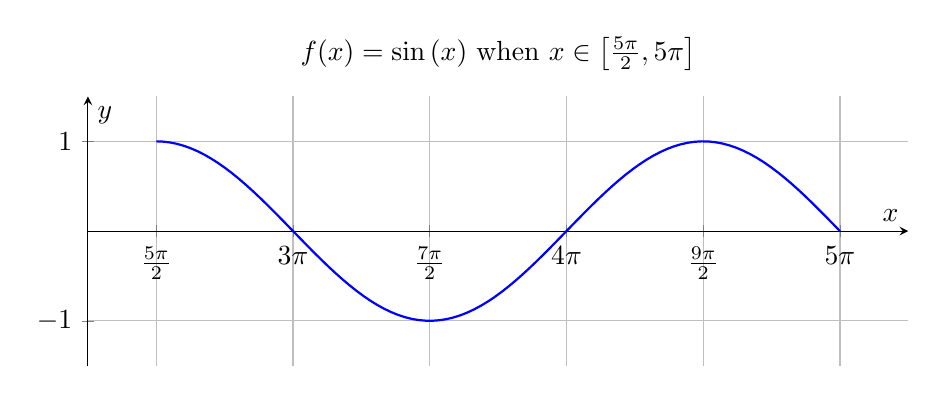
\begin{tikzpicture}
        \begin{axis}[%
            title = {$f(x) = \sin\left(x\right)$ when $x \in \left[\frac{5\pi}{2}, 5\pi \right]$},
            xlabel = {$x$}, ylabel = {$y$},
            xmin = (4.5 / 2) * pi, xmax = {5.25 * pi},
            ymin = -1.5, ymax = 1.5,
            xtick = {
                (5 * pi) / 2,
                3 * pi,
                (7 * pi) / 2,
                4 * pi,
                (9 * pi) / 2,
                5 * pi%
                },
            xticklabels = {
                $\frac{5\pi}{2}$,
                $3\pi$,
                $\frac{7\pi}{2}$,
                $4\pi$,
                $\frac{9\pi}{2}$,
                $5\pi$%
            },
            ytick = {
                -1,
                1
            },
            axis lines = center, grid = both,
            width = 12cm, height = 5cm,
            trig format plots=rad
        ]
        \addplot[color = blue, thick, domain = {(5 * pi) / 2}:{5 * pi}, samples = 100]{sin(x)};
        \end{axis}
    \end{tikzpicture}
\end{center}
This problem is challenging because I didn't give the value of $f(x)$ for $x = 0$ \textit{or} $x = 2\pi$. However, the method you use for finding the period is the exact same. In this example, I'll use the value of $f(x)$ when $x = 3\pi$.

When $x = 3\pi$, the function has a $y$ value of $y = 0$ and is pointing down. That means I need to find the first occurance of the function that returns to a height of $y = 0$ and also points down. That happens at $x = 5\pi$.

Now, to find the period, I just need to subtract the first occurance by the initial observation. That means $5\pi - 3\pi$. Subtracting gives a period of $2\pi$.

As you get better at determining the period of a trigonometric function, you won't even need much to identify. With the previous example, for instance, we could find the period in a different way.

Step 1: Observe that the function has a height of $y = 1$ and points down when $x = \frac{5\pi}{2}$.

Step 2: Observe that the function reaches a height of $y = 0$ at $x = 3\pi$.

Step 3: Remember that a sine function ossilates smoothly and evenly between $y = -1$ and $y = 1$. That means, if we started at $y = 1$ and ended at $y = 0$ after moving horizontally by $\frac{\pi}{2}$, we can predict what the graph will look like.
\begin{center}
    \begin{minipage}[c]{0.3\linewidth}
        \begin{tabular}{ c | c }
            $x$ & $f(x) = \sin(x)$ \\
            \hline
            $\frac{5\pi}{2}$ & $1$ \\
            \hline
            $3\pi$ & $0$ \\
            \hline
            $\frac{7\pi}{2}$ & $-1$ \\
            \hline
            $4\pi$ & $0$ \\
            \hline
            $\frac{9\pi}{2}$ & $1$ \\
        \end{tabular}
    \end{minipage}
    \begin{minipage}[c]{0.69\linewidth}
        Step 4: With this table, observe that the height of the function at $x = \frac{9\pi}{2}$ is $y = 1$, which is the same height at $x = \frac{5\pi}{2}$. 
        \\ \\
        Step 5: Take $\frac{9\pi}{2} - \frac{5\pi}{2}$ to find the period. When we subtract, we get $\frac{4\pi}{2}$, which is $2\pi$. 
    \end{minipage}
\end{center}
We got the same result as before, but with only $\frac{\pi}{2}$ of the graph to work with.
\clearpage
\section{Properties Of The Tangent Function}
The tangent function, like sine and cosine, has a period. But it's much easier to determine. Take a loog at the tangent function.
\begin{center}
    \begin{minipage}[c]{0.42\linewidth}
        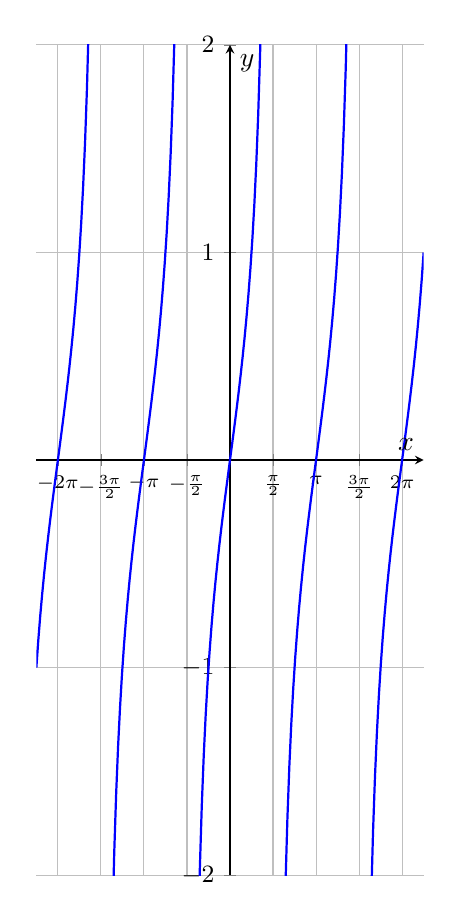
\begin{tikzpicture}
            \begin{axis}[%
                xlabel = {$x$}, ylabel = {$y$},
                xmin = {-1 * 9/4*pi}, xmax = {9/4*pi},
                ymin = -2, ymax = 2,
                restrict y to domain=-10:10,
                xtick = {
                    -2 * pi,
                    -3 / 2 * pi,
                    -1 * pi,
                    -1 / 2 * pi,
                    0, 
                    pi / 2, 
                    pi, 
                    (3 * pi) / 2,
                    2 * pi%
                    },
                xticklabels = {
                    $-2\pi$,
                    $-\frac{3\pi}{2}$,
                    $-\pi$,
                    $-\frac{\pi}{2}$,
                    $0$,
                    $\frac{\pi}{2}$,
                    $\pi$,
                    $\frac{3\pi}{2}$,
                    $2\pi$%
                },
                ytick = {
                    -2,
                    -1,
                    1,
                    2%
                },
                x tick label style = {font=\scriptsize},
                y tick label style = {font=\small},
                axis lines = center, grid = both,
                width = 6.5cm, height = \linewidth,
                trig format plots=rad
            ]
            \addplot[color = blue, thick, domain = {-1 * 9/4*pi}:{9/4*pi}, samples = 200]{tan(x)};
            \end{axis}
        \end{tikzpicture}
    \end{minipage}
    \begin{minipage}[c]{0.57\textwidth}
        Notice how it follows a consistent pattern. Each segment starts at $-\infty$, crosses the $x$-axis line at some $x = n\pi$, and then shoots up to $\infty$. And then the pattern repeats.
        \\ \\
        This pattern is why it's so easy to find the period of this function. It's just the distance between asymptotes.
    \end{minipage}
\end{center}
\begin{center}
    \begin{minipage}[c]{0.57\linewidth}
        Look at this snippet of the tangent function from $x = \frac{\pi}{2}$ to $x = \frac{3\pi}{2}$. The asymptote on the left is at $x = \frac{\pi}{2}$. The asymptote on the right is $\frac{3\pi}{2}$. So, to find the period of this, we just subtract the right asymptote by the left.
        \[
            \frac{3\pi}{2} - \frac{\pi}{2} = \pi
        \]
    \end{minipage}
    \begin{minipage}[c]{0.42\textwidth}
        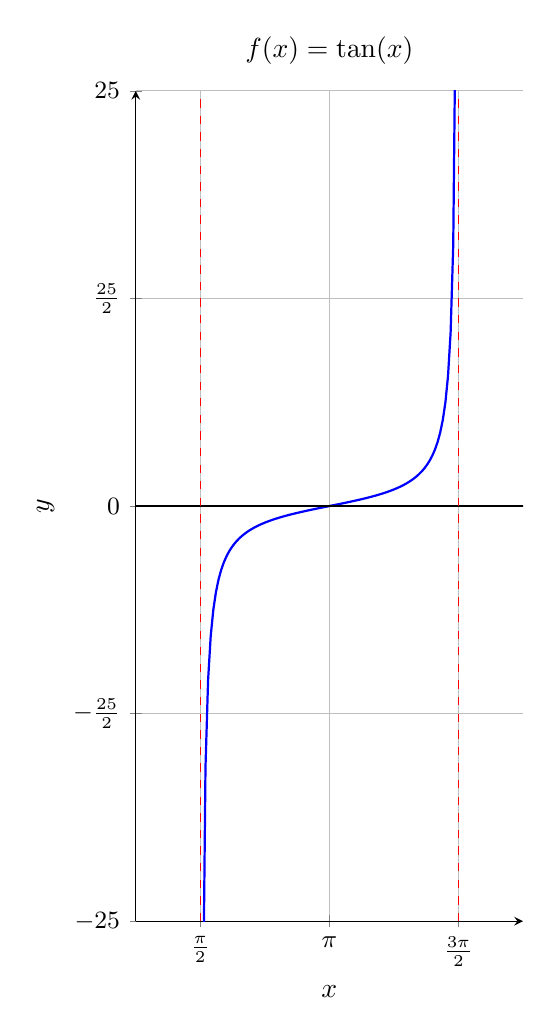
\begin{tikzpicture}
            \begin{axis}[%
                title = {$f(x) = \tan(x)$},
                xlabel = {$x$}, ylabel = {$y$},
                xmin = {pi / 4}, xmax = {(7 / 4) * pi},
                ymin = -25, ymax = 25,
                restrict y to domain=-50:50,
                xtick = {
                    -2 * pi,
                    -3 / 2 * pi,
                    -1 * pi,
                    -1 / 2 * pi,
                    0, 
                    pi / 2, 
                    pi, 
                    (3 * pi) / 2,
                    2 * pi%
                    },
                xticklabels = {
                    $-2\pi$,
                    $-\frac{3\pi}{2}$,
                    $-\pi$,
                    $-\frac{\pi}{2}$,
                    $0$,
                    $\frac{\pi}{2}$,
                    $\pi$,
                    $\frac{3\pi}{2}$,
                    $2\pi$%
                },
                ytick = {
                    -25,
                    -12.5,
                    0,
                    12.5,
                    25%
                },
                yticklabels = {
                    $-25$,
                    $-\frac{25}{2}$,
                    $0$,
                    $\frac{25}{2}$,
                    $25$%
                },
                x tick label style = {font=\small},
                y tick label style = {font=\small},
                axis lines = left, grid = both,
                width = 6.5cm, height = \linewidth,
                trig format plots=rad
            ]
            \addplot[color = blue, thick, domain = {pi / 2}:{(3/2) * pi}, samples = 100]{tan(x)};
            \draw[color = black] (0, 0) -- ({2 * pi}, 0);
            \draw[color = red, dashed] ({pi / 2}, {-25}) -- ({pi / 2}, 25);
            \draw[color = red, dashed] ({(3 / 2) * pi}, {-25}) -- ({(3 / 2) * pi}, 25);
            \end{axis}
        \end{tikzpicture}
    \end{minipage}
\end{center}
That makes the period of the function $f(x) = \tan(x)$ equal to $\pi$. That's about it. To find the period of the tangent function, you just see how far appart the asymptotes are from each other.
\clearpage
Let's try a different example.
\begin{problem}
    From the graph below, determine the period of this tangent function.
    \begin{center}
        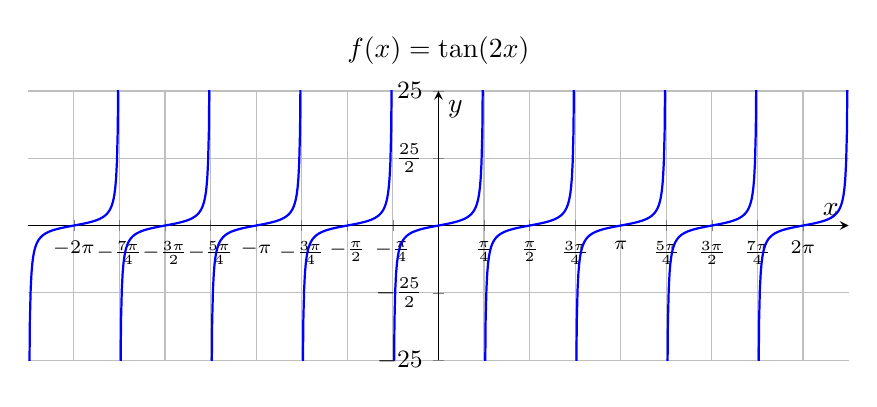
\begin{tikzpicture}
            \begin{axis}[%
                title = {$f(x) = \tan(2x)$},
                xlabel = {$x$}, ylabel = {$y$},
                xmin = {-1 * (9/4) * pi}, xmax = {9/4*pi},
                ymin = -25, ymax = 25,
                restrict y to domain=-100:100,
                xtick = {
                    -1 * 2 * pi,
                    -1 * (7 / 4) * pi,
                    -1 * (3 / 2) * pi,
                    -1 * (5 / 4) * pi,
                    -1 * pi,
                    -1 * (3 / 4) * pi,
                    -1 * (1 / 2) * pi,
                    -1 * (1 / 4) * pi,
                    0,
                    (1 / 4) * pi,
                    (1 / 2) * pi,
                    (3 / 4) * pi,
                    pi,
                    (5 / 4) * pi,
                    (3 / 2) * pi,
                    (7 / 4) * pi,
                    2 * pi%
                    },
                xticklabels = {
                    $-2\pi$,
                    $-\frac{7\pi}{4}$,
                    $-\frac{3\pi}{2}$,
                    $-\frac{5\pi}{4}$,
                    $-\pi$,
                    $-\frac{3\pi}{4}$,
                    $-\frac{\pi}{2}$,
                    $-\frac{\pi}{4}$,
                    $0$,
                    $\frac{\pi}{4}$,
                    $\frac{\pi}{2}$,
                    $\frac{3\pi}{4}$,
                    $\pi$,
                    $\frac{5\pi}{4}$,
                    $\frac{3\pi}{2}$,
                    $\frac{7\pi}{4}$,
                    $2\pi$%
                },
                ytick = {
                    -25,
                    -12.5,
                    12.5,
                    25%
                },
                yticklabels = {
                    $-25$,
                    $-\frac{25}{2}$,
                    $\frac{25}{2}$,
                    $25$%
                },
                x tick label style = {font=\scriptsize},
                y tick label style = {font=\small},
                axis lines = center, grid = both,
                width = 12cm, height = 5 cm,
                trig format plots=rad
            ]
            \addplot[color = blue, thick, domain = {-1 * 9/4*pi}:{9/4*pi}, samples = 1000] {tan(2 * x)};
            \end{axis}
        \end{tikzpicture}
    \end{center}
\end{problem}
\begin{solution}
    \begin{center}
        \begin{minipage}[c]{0.5\linewidth}
            \begin{tikzpicture}
                \begin{axis}[%
                    xlabel = {$x$}, ylabel = {$y$},
                    xmin = pi / 4, xmax = (3 * pi) / 4,
                    ymin = -25, ymax = 25,
                    restrict y to domain=-50:50,
                    xtick = {
                        -2 * pi,
                        -3 / 2 * pi,
                        -1 * pi,
                        -1 / 2 * pi,
                        0, 
                        pi / 2, 
                        pi, 
                        (3 * pi) / 2,
                        2 * pi%
                        },
                    xticklabels = {
                        $-2\pi$,
                        $-\frac{3\pi}{2}$,
                        $-\pi$,
                        $-\frac{\pi}{2}$,
                        $0$,
                        $\frac{\pi}{2}$,
                        $\pi$,
                        $\frac{3\pi}{2}$,
                        $2\pi$%
                    },
                    ytick = {
                        -25,
                        -12.5,
                        0,
                        12.5,
                        25%
                    },
                    yticklabels = {
                        $-25$,
                        $-\frac{25}{2}$,
                        $0$,
                        $\frac{25}{2}$,
                        $25$%
                    },
                    x tick label style = {font=\small},
                    y tick label style = {font=\small},
                    axis lines = middle, grid = both,
                    width = \linewidth, height = \linewidth,
                    trig format plots=rad
                ]
                \addplot[color = blue, thick, domain = {pi / 4}:{(3 / 4) * pi}, samples = 200]{tan(2 * x)};
                \end{axis}
            \end{tikzpicture}
        \end{minipage}
        \begin{minipage}[c]{0.45\textwidth}
            Notice how it follows a consistent pattern. Each segment starts at $-\infty$, crosses the $x$-axis line at some $x = n\pi$, and then shoots up to $\infty$. And then the pattern repeats.
            \\ \\
            This pattern is why it's so easy to find the period of this function. It's just the distance between asymptotes.
        \end{minipage}
    \end{center}
    Looking at the first blue line in the positive $x$ direction, we see that the left asymptote is at $x = \frac{\pi}{4}$ and the right asymptote is at $x = \frac{3\pi}{4}$.
    \[
        \frac{3\pi}{4} - \frac{\pi}{4} = \frac{2\pi}{4} = \frac{\pi}{2}
    \]
    Thus, the period of this function is $\frac{\pi}{2}$.
\end{solution}
\clearpage
\section{Frequency}
The frequency of a trigonometric function is defined as the reciprocal of its period. For example, if the period of a function is $2\pi$, it's frequency is $\frac{1}{2\pi}$. To generalize:
\begin{definition}
    The frequency of a trigonometric function is
    \[
        P^{-1} \text{ or } \frac{1}{P} \text{,}
    \]
    where $P$ is the period of the function.
\end{definition}
If the period of a function is how long it takes for it to complete one full cycle, the frequency of a function is how much of the cycle was reached in some interval (usually $1$ unit).

To demonstrate, I'll use the function $\cos(x)$. In the section on the period of sine and cosine, we learn that $\cos(x)$ has a period of $2\pi$. We take the reciprocal of this to find that its frequency is $\frac{1}{2\pi}$, which is approximately $0.159155$. This means that, after one radian, routhly $15.9155\%$ of the cycle is completed.

In other words, if you separated $\cos(x)$ in the interval $x \in [0, 2\pi]$ into subintervals that are $1$ unit long, you'd end up with $2\pi \approx 6.283185$ intervals. The below graph demonstrates this.
\begin{center}
    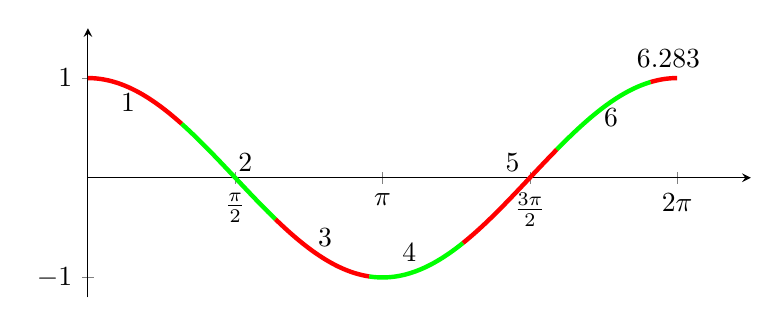
\begin{tikzpicture}
        \begin{axis}[%
            xmin = 0, xmax = (9 * pi) / 4,
            ymin = -1.2, ymax = 1.5,
            xtick = {
                0,
                pi / 2,
                pi,
                (3 * pi) / 2,
                2 * pi%
            },
            xticklabels = {
                $0$,
                $\frac{\pi}{2}$,
                $\pi$,
                $\frac{3\pi}{2}$,
                $2\pi$
            },
            width = 10cm, height = 5cm,
            trig format plots=rad,
            axis lines = center%
        ]
        \addplot[color = red, ultra thick, domain = 0:1, samples = 100] {cos(x)};
        \node[right] at (0.25, 0.75) {$1$};
        
        \addplot[color = green, ultra thick, domain = 1:2, samples = 100] {cos(x)};
        \node[right] at (1.5, 0.15) {$2$};

        \addplot[color = red, ultra thick, domain = 2:3, samples = 100] {cos(x)};
        \node[right] at (2.35, -0.6) {$3$};

        \addplot[color = green, ultra thick, domain = 3:4, samples = 100] {cos(x)};
        \node[right] at (3.25, -0.75) {$4$};

        \addplot[color = red, ultra thick, domain = 4:5, samples = 100] {cos(x)};
        \node[right] at (4.35, 0.15) {$5$};

        \addplot[color = green, ultra thick, domain = 5:6, samples = 100] {cos(x)};
        \node[right] at (5.4, 0.6) {$6$};

        \addplot[color = red, ultra thick, domain = 6:{2 * pi}, samples = 100] {cos(x)};
        \node[right] at (5.75, 1.2) {$6.283$};
        \end{axis}
    \end{tikzpicture}
\end{center}
This idea can be extended to any period, hence the definition. Also, because of the direction relationship between the period and frequency of a trigonometric function, we can solve for one if we have the other.
\clearpage
In the example above, we used the period to find the frequency. However, if we have the frequency, we can find the period with a little algebra.
\[
    \text{If } F = \frac{1}{P}\text{, then } P = \frac{1}{F} \text{.}
\]
Try this for size:
\begin{problem}
    Given the the frequency of some trigonometric function $f$ is $0.384$, find the period $P$ of the function.
\end{problem}
\begin{solution}
    All we need to do to find the period is the take the reciprocal of this frequency. If $F = 0.384$, then
    \begin{align*}
        P = \frac{1}{0.384} = \frac{1000}{384} = \frac{125}{48} \approx 2.604167
    \end{align*}
\end{solution}

\clearpage
\chapter{Special Triangles}
Special triangles are something you likely looked at back in geometry. However, they will serve a fundamental role in the next chapter when I talk about the unit circle. The two I'll look at in this chapter are the 30-60-90 and the 45-45-90 triangles. Special triangles are called "special triangles" because they're easy to solve for. The ratios for all the sides and angles are known. So, if you have one (side or angle) you have all of them.

The numbers in the names of these triangles refers to the values of the three angles. I'll begin with the 30-60-90 triangle and continue with the 45-45-90.
\section{The 30-60-90 Triangle}
The 30-60-90 triangle is a right triangle that has one angle of $30\degree$, one angle of $60\degree$, and a right angle ($90\degree$).
\begin{center}
    \begin{minipage}[c]{0.45\linewidth}
        \centering
        \captionof{figure}{30-60-90 Triangle}
        \label{fig:30-60-90}
        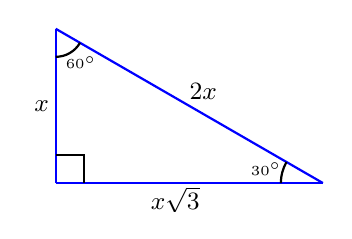
\begin{tikzpicture}
            \begin{axis}[
                xmin = -10, xmax = 100,
                ymin = -10, ymax = 100,
                height = 5.5cm, width = 5.5cm,
                axis lines = none%
            ]
                %Triangle
                \draw[color = blue, thick] (0,0) -- (0,55);
                \draw[color = blue, thick] (0,55) -- ({55 / tan(30)}, 0);
                \draw[color = blue, thick] (0,0) -- ({55 / tan(30)}, 0);

            % 30 Degree Angle
            \node[font = \tiny] at (75, 5) {$30\degree$};
            \draw[color = black, thick] ({(55 / tan(30)) - 15},0) arc (180:150:15);

            % 60 Degree Angle
            \node[font = \tiny] at (9,43) {$60\degree$};
            \draw[color = black, thick] (0, {55-10}) arc (270:330:10);

            %Side Labels
            \node[font = \small] at (-5, {55 / 2}) {$x$};                                   % x label 
            \node[font = \small] at ({55 / (2 * tan(30)) - 5}, -6) {$x\sqrt{3}$};           % xsqrt(3) label
            \node[font = \small] at ({55 / (2 * tan(30)) + 5}, {(55 / 2) + 5}) {$2x$};     % 2x label

            % Right angle symbol
            \draw[thick, color = black] (0,10) -- (10,10) -- (10,0);
            \end{axis}
        \end{tikzpicture}
    \end{minipage}
    \begin{minipage}[c]{0.50\linewidth}
        Regardless of the size and orientation of a 30-60-90 triangle, the side proportions and angle measurements will remain the same. When comparing to the short leg (vertical), the other leg is longer by a factor of $\sqrt{3}$ and the hypotenuse by $2$.\\\\Also note that the smaller leg is opposite the smaller angle!!
    \end{minipage}
\end{center}
\clearpage
You may also see this triangle depicted as having a short leg of length $1$, a long leg of length $\sqrt{3}$, and a hypotenuse of length $2$. It's exactly the same as the one shown in Figure \ref{fig:30-60-90}. It just has $x$ set equal to $1$.

\section{The 45-45-90 Triangle}
The 45-45-90 triangle is a right triangle that has two angles of $45\degree$ and a right angle ($90\degree$).
\begin{center}
    \begin{minipage}[c]{0.45\linewidth}
        \centering
        \captionof{figure}{45-45-90 Triangle}
        \label{fig:45-45-90}
        \begin{tikzpicture}
            \begin{axis}[
                xmin = -10, xmax = 100,
                ymin = -10, ymax = 100,
                height = 5.5cm, width = 5.5cm,
                axis lines = none%
            ]
            %Triangle
            \draw[color = blue, thick] (0,0) -- (0,55);
            \draw[color = blue, thick] (0,55) -- ({55 / tan(45)}, 0);
            \draw[color = blue, thick] (0,0) -- ({55 / tan(45)}, 0);

            % 30 Degree Angle
            \node[font = \tiny] at (40,5) {$45\degree$};
            \draw[color = black, thick] ({(55 / tan(45)) - 10},0) arc (180:135:10);

            % 60 Degree Angle
            \node[font = \tiny] at (6.5,41) {$45\degree$};
            \draw[color = black, thick] (0, {55-10}) arc (270:315:10);

            %Side Labels
            \node[font = \small] at (-5, {55 / 2}) {$x$};                                       % x label 
            \node[font = \small] at ({55 / (2 * tan(45)) - 5}, -6) {$x$};                       % xsqrt(3) label
            \node[font = \small] at ({55 / (2 * tan(45)) + 7}, {(55 / 2) + 7}) {$x\sqrt{2}$};   % 2x label

            % Right angle symbol
            \draw[thick, color = black] (0,10) -- (10,10) -- (10,0);
            \end{axis}
        \end{tikzpicture}
    \end{minipage}
    \begin{minipage}[c]{0.50\linewidth}
        Figure \ref{fig:45-45-90} shows a 45-45-90 triangle with all of the sides labeled. Regardless of the size and orientation of a 45-45-90 triangle, the side proportions and angle measurements will remain the same. The two legs of the triangle are equal in length, and the hypotenuse is longer by a factor of $\sqrt{2}$.
    \end{minipage}
\end{center}
You may also see this triangle depicted as having a two legs of length $1$ and a hypotenuse of length $\sqrt{2}$. It's exactly the same as the one shown in Figure \ref{fig:45-45-90}. It just has $x$ set equal to $1$.
\section*{Practice Problems}
Let's try solving for some of these triangles.
\begin{problem}
    If you're given a 30-60-90 triangle with a hypotenuse of $10$ units, what must the legs of the triangle be?
\end{problem}
\begin{solution}
    A 30-60-90 triangle has a short leg of $x$, a long leg of length $x\sqrt{3}$, and a hypotenuse of $2x$. In this example, we're given that the hypotenuse, which is equal to $2x$, is $10$ units.

    In other words, this question is asking: If $10 = 2x$, the short leg is equal to $x$, and the long leg is equal to $x\sqrt{3}$, what are $x$ and $x\sqrt{3}$? To answer this, we just need to find the value of $x$.

    We're given an equation $10 = 2x$. Solving this for $x$ answers the question.
    \[
        10 = 2x \Longrightarrow x = 5
    \]
    This means the hypotenuse is $10$ units, the short leg is $5$ units, and the long leg is $5\sqrt{3}$ units.
\end{solution}
\begin{problem}
    If the leg adjacent to the $30\degree$ angle of a right triangle has a length of $3$ units, what must the length of the other leg and hypotenuse be?
\end{problem}
\begin{solution}
    To solve, we must confirm what triangle we're actually working with. Recall that the angles of a triangle \textbf{must} add up to $180$ degrees. 
    
    The problem gives a $30\degree$ angle and states that the triangle is a \textbf{right} triangle. That means we're actually given two angles: a $30\degree$ angle (stated explicitly) and a $90\degree$ angle (the right angle of a right triangle).

    Adding $30$ and $90$ gives $120$, and subtracting $120$ from $180$ (i.e. $180 - 120$) gives $60$. Confirming that our third angle is $60\degree$ also confirms that we're working with a 30-60-90 triangle.

    Looking back at the problem, we see that "the leg adjacent to the $30\degree$ angle has a length of $3$ units." That's the leg colored in red.
    \begin{center}
        \begin{minipage}[c]{0.45\linewidth}
            \centering
            \begin{tikzpicture}
                \begin{axis}[
                    xmin = -10, xmax = 100,
                    ymin = -10, ymax = 100,
                    height = 5.5cm, width = 5.5cm,
                    axis lines = none%
                ]
                    %Triangle
                    \draw[color = blue, thick] (0,0) -- (0,55);
                    \draw[color = blue, thick] (0,55) -- ({55 / tan(30)}, 0);
                    \draw[color = red, thick] (0,0) -- ({55 / tan(30)}, 0);

                % 30 Degree Angle
                \node[font = \tiny] at (75, 5) {$30\degree$};
                \draw[color = black, thick] ({(55 / tan(30)) - 15},0) arc (180:150:15);

                % 60 Degree Angle
                \node[font = \tiny] at (9,43) {$60\degree$};
                \draw[color = black, thick] (0, {55-10}) arc (270:330:10);

                %Side Labels
                \node[font = \small] at ({55 / (2 * tan(30)) - 5}, -6) {$3$ units};           % xsqrt(3) label

                % Right angle symbol
                \draw[thick, color = black] (0,10) -- (10,10) -- (10,0);
                \end{axis}
            \end{tikzpicture}
        \end{minipage}
        \begin{minipage}[c]{0.50\linewidth}
            Since we know from looking at Figure \ref{fig:30-60-90} that the longer leg is $x\sqrt{3}$ units long, we can actually solve for $x$ and find the value of the shorter leg and hypotenuse.
        \end{minipage}
    \end{center}
    Let's start by setting $x\sqrt{3}$ equal to $3$ and solving for $x$.
    \begin{align*}
        x\sqrt{3} &= 3 \\
        x &= \frac{3}{\sqrt{3}} \\
        x &= \frac{3\sqrt{3}}{3} \\
        x &= \sqrt{3}
    \end{align*}
    The $x$ we just found is the length of the shorter leg. Since the hypotenuse is known to be $2x$ in length, doubling this gives us the length of the hypotenuse.
    \begin{align*}
        \sqrt{3} \cdot 2 &= 2\sqrt{3}
    \end{align*}
    That gives us the triangle below.
    \begin{center}
        \centering
        \begin{tikzpicture}
            \begin{axis}[
                xmin = -20, xmax = 100,
                ymin = -10, ymax = 100,
                height = 5.5cm, width = 5.5cm,
                axis lines = none%
            ]
                %Triangle
                \draw[color = blue, thick] (0,0) -- (0,55);
                \draw[color = blue, thick] (0,55) -- ({55 / tan(30)}, 0);
                \draw[color = blue, thick] (0,0) -- ({55 / tan(30)}, 0);

            % 30 Degree Angle
            \node[font = \tiny] at (75, 5) {$30\degree$};
            \draw[color = black, thick] ({(55 / tan(30)) - 15},0) arc (180:150:15);

            % 60 Degree Angle
            \node[font = \tiny] at (9,43) {$60\degree$};
            \draw[color = black, thick] (0, {55-10}) arc (270:330:10);

            %Side Labels
            \node[font = \small] at (-10, {55 / 2}) {$\sqrt{3}$};                         % x label 
            \node[font = \small] at ({55 / (2 * tan(30)) - 5}, -6) {$3$};                           % xsqrt(3) label
            \node[font = \small] at ({55 / (2 * tan(30)) + 6.5}, {(55 / 2) + 6.5}) {$2\sqrt{3}$};       % 2x label

            % Right angle symbol
            \draw[thick, color = black] (0,10) -- (10,10) -- (10,0);
            \end{axis}
        \end{tikzpicture}
    \end{center}
\end{solution}
\begin{problem}
    Given an isosceles right triangle with a hypotenuse of $4$ units, find the length of its two legs.
\end{problem}
\begin{solution}
    Let's look at what we're given.
    \begin{enumerate}
        \item We're given that this is a right triangle, meaning it must have one angle of $90\degree$.
        \item We're given that the hypotenuse of this triangle is $4$ units.
        \item We're given that this triangle is not only a right triangle, but an isosceles triangle. This means that the two legs are the same length.
    \end{enumerate}
    \clearpage
    With the given information, we can see that we're working with a 45-45-90 triangle. We have a $90\degree$ angle and two sides that are the same length. That exactly matches the two legs of length $x$ seen in Figure \ref{fig:45-45-90}. Also from that figure, recall that the hypotenuse has a length of $x\sqrt{2}$ units.

    With that, we can set $x\sqrt{2}$ equal to $4$ and solve for $x$.
    \begin{align*}
        x\sqrt{2} &= 4 \\
        x &= \frac{4}{\sqrt{2}} \\
        &= \frac{4\sqrt{2}}{2} \\
        &= 2\sqrt{2}
    \end{align*}
    The $x$ we just solved for is the length of both legs (since they're the same length). That also means we're done.
    \begin{center}
        \begin{tikzpicture}
            \begin{axis}[
                xmin = -20, xmax = 100,
                ymin = -10, ymax = 100,
                height = 5.5cm, width = 5.5cm,
                axis lines = none%
            ]
            %Triangle
            \draw[color = blue, thick] (0,0) -- (0,55);
            \draw[color = blue, thick] (0,55) -- ({55 / tan(45)}, 0);
            \draw[color = blue, thick] (0,0) -- ({55 / tan(45)}, 0);

            % 30 Degree Angle
            \node[font = \tiny] at (40,5) {$45\degree$};
            \draw[color = black, thick] ({(55 / tan(45)) - 10},0) arc (180:135:10);

            % 60 Degree Angle
            \node[font = \tiny] at (6.5,41) {$45\degree$};
            \draw[color = black, thick] (0, {55-10}) arc (270:315:10);

            %Side Labels
            \node[font = \small] at (-11, {55 / 2}) {$2\sqrt{2}$};                                       % x label 
            \node[font = \small] at ({55 / (2 * tan(45)) - 5}, -6) {$2\sqrt{2}$};                       % xsqrt(3) label
            \node[font = \small] at ({55 / (2 * tan(45)) + 5}, {(55 / 2) + 5}) {$4$};   % 2x label

            % Right angle symbol
            \draw[thick, color = black] (0,10) -- (10,10) -- (10,0);
            \end{axis}
        \end{tikzpicture}
    \end{center}
\end{solution}
Let's look at one last problem that's a bit different from the rest before continuing. As always, I encourage you to try the problem yourself before looking at the solution.
\begin{problem}
    Determine the type of special triangle that has side lengths of $3$, $4$, and $5$ units.
\end{problem}
\begin{solution}
    The two types of special triangles we've covered are the 30-60-90 and the 45-45-90. First and foremost, let's confirm whether this triangle is even a right triangle.

    To do this, we'll use the Pythagorean Theorem ($a^2 + b^2 = c^2$). If this equation holds, then we can continue to the next step.
    \clearpage
    I'll define $a = 3$, $b = 4$, and $c = 5$. The order of $a$ and $b$ do not matter because they are the legs. However, $c$ \textbf{must} be $5$. The length of $5$ units is the longest of the three, so it \textbf{must} be the hypotenuse.

    Substituting those values in gives:
    \begin{align*}
        3^2 + 4^2 &= 5^2 \\
        9 + 16 &= 25 \\
        25 &= 25
    \end{align*}
    The Pythagorean Theorem holds, so we've confirmed that this triangle is a right triangle and can continue to the next part of the solution.

    First, let's test to see if this is a 30-60-90 triangle. Recall that the short leg has a length of $x$, the long leg has a length of $x\sqrt{3}$, and the hypotenuse has a length of $2x$.

    In the given triangle, the short leg ($x$) is $3$, the long leg is $4$, and the hypotenuse is $5$. That means:
    \begin{itemize}
        \item $x = 3$
        \item $x\sqrt{3} = 4$
        \item $2x = 5$
    \end{itemize}
    Since we're already given that $x = 3$, let's try plugging that into the other two equations.
    \begin{align*}
        3\sqrt{3} \neq 4 \qquad 2(3) = 6 \neq 5
    \end{align*}
    Since a value of $x = 3$ doesn't make sense given the side lengths, we can say that this is not a 30-60-90 triangle.

    Now, let's see whether this is a 45-45-90 triangle. Same as before, we'll state the side lengths.
    \begin{itemize}
        \item $x = 3$ (leg 1)
        \item $x = 4$ (leg 2)
        \item $x\sqrt{2} = 5$ (hypotenuse)
    \end{itemize}
    This fails immediately. We have an $x = 3$ \textbf{and} and $x = 4$. Therefore, this is also not a 45-45-90 triangle.

    This was actually a trick question. The triangle described isn't a special triangle at all. It's actually what's referred to as a \textbf{Pythagorean Triple}, meaning all three sides are integers and form a right triangle.

    Other examples of Pythagorean Triples are the 8-15-17 and 12-35-37. However, the 3-4-5 triple is most commonly used.
\end{solution}
\end{document}